\documentclass[
  12pt,
  headsepline,
]{scrartcl}
\usepackage{graphicx}
\usepackage{physics}
\graphicspath{{./Bilder/}}
\usepackage[utf8]{inputenc}
\usepackage[T1]{fontenc}
\usepackage{amsmath,amsfonts,amssymb}
\usepackage{stmaryrd} 
\usepackage[ngerman]{babel}
\usepackage{microtype}
\renewcommand{\listfigurename}{Abbildungsverzeichnis}
\usepackage{minted}
  \renewcommand\listingscaption{Quellcode}
  \renewcommand\listoflistingscaption{Quellcodeverzeichnis}
  \usepackage{scrhack} % Uses KOMA deprecated float@listhead
\usepackage{csquotes}
\usepackage{amsmath}
\usepackage{acronym}
\usepackage{mathtools}
\usepackage{url}
\usepackage{hyperref}
\hypersetup{
  pdfauthor={},
  pdftitle={},
  pdfsubject={Bachelorarbeit},
  pdfkeywords={Bachelorarbeit}
}

\bibliographystyle{IEEEtran}
\usepackage[style=alphabetic]{biblatex}
\addbibresource{BA_Bib.bib}

% Bilder, Code-Blöcke, Farben, ...
\usepackage{float}
\usepackage{listings}
\lstset{
  showstringspaces=false,
  frame=lines,
  breaklines=true,
  language=Python,
  captionpos=b,
  prebreak={\Righttorque},
  basicstyle=\ttfamily
}
\usepackage{xcolor}

% Logo auf der Titelseite
\usepackage[absolute]{textpos}
\setlength{\TPHorizModule}{1mm}
\setlength{\TPVertModule}{\TPHorizModule}
\textblockorigin{0mm}{0mm}

\hyphenation{
  Ad-mi-nis-tra-tor
  Get-Re-quest
  Get-Re-sponse
  Get-Next-Request
  Get-Bulk-Request
  Pro-gram-mie-rung
  fast-ether-net
  hexa-de-zi-mal-en
}

\DeclareMathOperator{\Landau}{\mathcal{O}}
\DeclareMathOperator{\Tensor}{\bigotimes}
\DeclareMathOperator{\tensor}{\otimes}

\begin{document}

\begin{titlepage}

\thispagestyle{empty}%
\setlength{\oddsidemargin}{0cm}%
\enlargethispage{\baselineskip}
\begin{textblock}{20}(188,8)%
    
\includegraphics[width=1.5cm]{fh_logo_rechts.png}%
 \end{textblock}%
\vspace*{-1.0cm}
\noindent
\LARGE\textbf{FH Aachen}\\
\Large\textbf{Fachbereich Elektrotechnik und Informationstechnik}\\
\large Prof. Dr. Marko Schuba
\vspace{2cm}
\begin{center}
	\LARGE\textbf{Bachelorarbeit}\\
	\vspace{1.75cm}
	\LARGE Implementierung einer Bibliothek von Quantenalgorithmen zur Kryptoanalyse\\
	\large
	\vspace{2.5cm}
	Eingereicht von:\\
	Simon Maximilian Kalytta\\
	Matrikelnummer: 3190683\\
	\vspace{1cm}
	Studienrichtung: Informatik\\
	\vspace{1cm}
	\today\\
	\vspace{1.5cm}
	Betreuerin: B.Sc. Janis König\\
	Prüfer: Prof. Dr. Marko Schuba\\
        \vspace{0.5cm}
        In Kooperation mit it.sec GmbH
\end{center}
\end{titlepage}


\section*{Kurzfassung}
In den vergangenen Jahren haben sich in der Entwicklung von Quantencomputern bedeutsame Fortschritte ergeben.
Aufgrund dieser Fortschritte erwarten Prognosen, 
dass in absehbarer Zukunft Quantencomputer mit kryptografisch relevanter Rechenleistung existieren könnten. 
Derzeit existieren bereits konzeptuelle Quantenalgorithmen, die in der Lage sind, 
bestimmte mathematische Probleme effizient zu lösen. 
Diese mathematischen Probleme spielen aufgrund ihrer Komplexität eine grundlegende Rolle in bestimmten Kryptosystemen. 
Da bisher keine Quantencomputer mit ausreichender Rechenleistung existieren, 
gibt es auch wenige konkrete Implementierungen dieser Quantenalgorithmen.

In dieser Arbeit wird der \textit{Shor-Algorithmus} zusammen mit verschiedenen Optimierungen 
auf der Abstraktionsebene von Quantenschaltkreisen implementiert.
Mithilfe dieses Quantenalgorithmus ist es möglich, 
die Primfaktorzerlegung mit einem vertretbaren Laufzeitaufwand zu berechnen. 
Alle bisher bekannten konventionellen klassischen Algorithmen zeigen bei dieser Berechnung eine exponentielle Laufzeitsteigerung, 
wobei das Wachstum der Laufzeit von der Größe der zu faktorisierenden Zahl abhängt.
Dementsprechend ist die Sicherheit von Kryptosystemen wie beispielsweise dem RSA-Verfahren, 
die auf der Schwierigkeit der Primfaktorzerlegung basieren, 
durch den \textit{Shor-Algorithmus} gefährdet.

Die in dieser Arbeit durchgeführte Implementierung des \textit{Shor-Algorithmus} 
wird um mehrere Optimierungen erweitert, 
die in unterschiedlichen Kombinationen verschiedene Varianten des Quantenalgorithmus ergeben.  
Des Weiteren wird ein klassischer Algorithmus zur Nachberechnung entwickelt, 
der die Erfolgsrate des Quantenalgorithmus erhöht. 
In einer Analyse werden die Laufzeiten und 
der Ressourcenbedarf der implementierten Varianten anhand von Kriterien für kryptografische Angriffe durch Quantenalgorithmen bewertet.
In einem Vergleich mit den Ergebnissen vergleichbarer Arbeiten zeigt sich, 
dass eine der implementierten Varianten sowohl einen geringeren Ressourcenbedarf als auch eine kürzere Laufzeit aufweist. 
Dennoch erfüllt keine der Varianten die Kriterien in Bezug auf die Laufzeit, 
um als effiziente Methode für empfohlene aktuelle Schlüssellängen betrachtet zu werden.

\bigbreak
\noindent
\textbf{Schlagwörter:} \textit{Shor-Algorithus},\textit{Quanten-Computing}, \textit{Qiskit}, \textit{RSA}, \textit{Primfaktorzerlegung}

\section*{Abstract}

In recent years, 
significant progress has been made in the development of quantum computers. 
These advancements have led to predictions that quantum computers with cryptographically relevant 
computational power could exist in the foreseeable future. 
Currently, there are already conceptual quantum algorithms capable of efficiently solving certain mathematical problems. 
Due to their complexity, 
these mathematical problems play a fundamental role in certain cryptographic systems. 
However, as of now, there are few concrete implementations of these quantum algorithms due 
to the lack of quantum computers with sufficient computational power.

In this thesis, 
the Shor algorithm, 
along with various optimizations at the abstraction level of quantum circuits, 
is implemented. Using this quantum algorithm, 
it becomes feasible to compute prime factorization with reasonable computational time. 
All known conventional classical algorithms exhibit exponential runtime growth in this computation, 
with the runtime growth depending on the size of the number to be factored. 
Consequently, the security of cryptographic systems, such as the RSA algorithm, 
which relies on the difficulty of prime factorization, is compromised by the Shor algorithm.

The implementation of the Shor algorithm in this work is extended with several optimizations that result in different variants of 
the quantum algorithm when combined in various ways. 
Furthermore, a classical post-processing algorithm is developed to increase the success rate of the quantum algorithm. 
An analysis evaluates the runtimes and resource requirements of the 
implemented variants based on criteria for cryptographic attacks by quantum algorithms. 
A comparison with the results of similar works reveals that one of the implemented variants exhibits both lower resource requirements and shorter runtime. 
However, none of the variants meet the criteria regarding runtime to be considered an efficient method for recommended current key lengths.

\bigbreak
\noindent
\textbf{Keywords:} \textit{Shor-Algorithm},\textit{Quantum-Computing}, \textit{Qiskit}, \textit{RSA}, \textit{Prime factorization}

\clearpage

\tableofcontents			% Inhaltsverzeichnis
%\listoftables				% Tabellenverzeichnis
\listoffigures				% Abbildungsverzeichnis
\listoflistings       % Codeverzeichnis
%\printnomenclature			% Abkürzungsverzeichnis

\section*{Abkürzungsverzeichnis}
\markright{Abkürzungsverzeichnis} 
%\begin{acronym}[Abkürzungen]
%	\acro{placeholder}{placeholder}
%	\acro{placeholder}{placeholder}
%\end{acronym}
\section*{Glossar}
\markright{Glossar} 



\section{Einleitung}

\subsection{Ziele und Vorgehen}
Das Ziel dieser Arbeit ist die Entwicklung und Implementierung einer auf Quantenalgorithmen 
basierenden Bibliothek zur Kryptoanalyse aktueller Verschlüsselungsverfahren. 
Angesichts des spezialisierten Fachwissens, das für die Entwicklung von Quantenalgorithmen erforderlich ist, 
konzentriert sich diese Arbeit auf die Implementierung und Anpassung eines in der Literatur bereits vorgestellten Quantenalgorithmus.
Der ausgewählte Quantenalgorithmus ist in der Lage, eine spezifische Problemstellung, 
die aufgrund ihrer Komplexität eine zentrale Rolle in modernen Verschlüsselungsverfahren einnimmt, 
deutlich effizienter zu lösen als die besten klassischen Algorithmen.

In der zugrunde liegenden wissenschaftlichen Literatur wird dieser Quantenalgorithmus als abstraktes oder konzeptuelles Modell beschrieben, 
ohne dass auf konkrete Implementierungsdetails eingegangen wird. 
Diese Arbeit beseitigt die Diskrepanz zwischen theoretischen Konzepten und praktischen Realisierungen, 
indem auf der Basis der abstrakten Konzepte eine konkrete Implementierung entwickelt wird.
Anschließend werden die resultierenden Implementierungen der Quantenalgorithmen mit klassischen Algorithmen kombiniert, 
um die Problemstellungen, die für die Sicherheit der Verschlüsselungsverfahren entscheidend sind, effektiv lösen zu können. 

Diese Arbeit implementiert die Bibliothek auf der Abstraktionsebene von Quantenschaltkreisen.
Dazu wird das Open-Source-Softwareentwicklungskit Qiskit genutzt, das auf der Programmiersprache Python basiert.

\subsection{Motivation}
In den letzten Jahren haben Fortschritte in der Forschung und Entwicklung von Quantencomputern neue Möglichkeiten für die praktische Untersuchung von Quantenalgorithmen ermöglicht.
Gegenwärtig ermöglichen sowohl Simulatoren von Quantencomputern als auch real existierende, wenn auch leistungsbegrenzte, Quantencomputer die Durchführung praktischer Tests.
Zur Zeit der ursprünglichen Konzeption der in dieser Arbeit verwendeten Quantenalgorithmen war eine praktische Erprobung entweder undenkbar oder nur durch umständliche Experimente mit stark vereinfachten Versuchen möglich.

Indem diese technologischen Möglichkeiten zur Ausführung und Erprobung der implementierten Quantenalgorithmen genutzt werden, 
eröffnet sich ein neuer Standpunkt, der die Betrachtung aus anderen Blickwinkeln erlaubt.


\subsection{Gliederung}
*Hier wird dann beschrieben in welchen Kapiteln der Leser welche Inhalte erwarten kann und wieso die Reihenfolge der Kapitel so gewählt wurden, inklusive der Struktur der Arbeit*



\section{Schwerpunkt}
\subsection{Entschlüsselungsfunktion für RSA} 
Der Fokus dieser Arbeit liegt auf der Implementierung einer Entschlüsselungsfunktion, die in der Lage ist, 
den privaten Schlüssel des RSA-Verfahrens aus dem zugehörigen öffentlichen Schlüssel abzuleiten.

Das RSA-Verfahren stellt ein sogenanntes asymmetrisches Kryptosystem dar.
Bei asymmetrischen Kryptosystemen kommt ein mathematisch verknüpftes Schlüsselpaar zum Einsatz. 
Dieses Schlüsselpaar besteht aus einem öffentlichen und einem privaten Schlüssel, 
wobei Letzterer ausschließlich dem Eigentümer des Schlüsselpaares zugänglich sein sollte.
Mit dem privaten Schlüssel ist der Eigentümer in der Lage, Nachrichten zu signieren. 
Ein Nutzer kann unter der Verwendung des öffentlichen Schlüssels die Authentizität der signierten Nachricht überprüfen. 
Hingegen erlaubt der öffentliche Schlüssel die Verschlüsselung von Nachrichten, 
deren anschließende Entschlüsselung ausschließlich mit dem privaten Schlüssel durchführbar ist.
Eine Bedingung der asymmetrischer Kryptosysteme ist, 
dass die Ableitung des privaten Schlüssels aus dem öffentlichen Schlüssel eine Herausforderung von erheblicher Komplexität darstellt~\cite{1055638}. 
Um dieser Anforderung gerecht zu werden, basieren asymmetrische Kryptosysteme auf mathematischen Problemstellungen, 
deren Lösung sogar mit dem Nutzen eines Computers von erheblicher Komplexität ist.

Die Sicherheit des kryptographischen Verfahren RSA beruht auf der Annahme,
dass die Faktorisierung eines Produkts bestehend aus zwei großen Primzahlen in keiner vertretbaren Zeit berechenbar ist.
Andernfalls wäre es möglich, aus dem öffentlichen Schlüssel die beiden Primfaktoren zu extrahieren, 
um anschließend damit den privaten Schlüssel zu bestimmen.
Daraus ergibt sich die Folgerung, dass, sofern die Faktorisierung großer Zahlen mit geringen Aufwand bewältigt werden kann, 
das RSA-Verfahren als kompromittiert angesehen werden muss~\cite{Cormen2009}.

Bislang ist kein klassischer Algorithmus bekannt, der die Primfaktorzerlegung effizient berechnen kann~\cite{Hoever2022Krypto}.
In diesem Zusammenhang bedeutet "'effizient"', dass die Laufzeit des Algorithmus in einem höchstens polynomialen Verhältnis zur Größe der Eingabezahl anwächst.

Im Kontext der Entschlüsselungsfunktion für RSA wird eine Funktion implementiert,
die in der Lage ist, die Primfaktorzerlegung effizient zu berechnen.
Zudem wird diese Funktion spezifisch darauf ausgerichtet, 
aus einem öffentlichen Schlüssel den zugehörigen privaten Schlüssel des RSA-Verfahrens abzuleiten.
Die Entschlüsselungsfunktion besteht aus einem Quantenalgorithmus und einem klassischer Algorithmus.
Der eingesetzte Quantenalgorithmus kann effektiv die Ordnung eines Elements in einer Gruppe bestimmen. 
Unter Einbeziehung der zuvor bestimmten Ordnung werden anschließend die Primfaktoren des öffentlichen Schlüssels mithilfe eines klassischen Algorithmus berechnet~\cite{Shor_1997}.
In einem abschließenden Schritt wird der private Schlüssel auf der Grundlage der berechneten Primfaktoren ermittelt.






\section{Quantencomputer}
\subsection{Entwicklung} 
Die Grundidee der Quantencomputer findet ihren Ursprung in dem Jahre 1980 als Paul Benioff ein theoretisches Modell einer klassischen Turing-Maschine beschrieb, 
die den Gesetzen der Quantenmechanik unterlag.
Benioff demonstrierte, dass die Zustände einer Turing-Maschine in einem Quantensystem darstellbar sind. 
Er zeigte außerdem, dass klassische Operationen, die in einer Turing-Maschine ausgeführt werden, 
durch entsprechende Quantengatter auf einem Quantensystem äquivalent durchgeführt werden können~\cite{benioff1980}.

Kurz nach der Veröffentlichung von Benioffs Arbeit beschäftigte sich Richard Feynman im Jahr 1981 mit der Frage,
wie effizient ein klassischer Computer bei der Simulation physikalischer Prozesse ist.
Feynman befasste sich mit der Schwierigkeit, die Quantenmechanik mithilfe eines klassischen Computers zu simulieren.
Er stellte fest, dass die Anforderungen für die Simulation der Quantenmechanik auf einem klassischen Computer mit jedem zusätzlichen Quantenteilchen exponentiell ansteigen.
Die Begründung dafür liegt in der exponentiell wachsenden Menge an Zustandsinformationen,
welche für die Beschreibung des Quantensystems benötigt werden.
Als Lösungsansatz nannte Feynman einen Quantencomputer, 
der selbst auf den Prinzipien der Quantenmechanik basiert und dadurch eine effiziente Simulation von Quantensystemen ermöglicht~\cite{Feynman1982}.

David Deutsch präsentierte im Jahr 1985 den ersten Quantenalgorithmus, 
der eine spezifische Fragestellung effizienter lösen konnte als jegliche bekannten klassischen Algorithmen. 
Allerdings bezog sich diese Fragestellung auf ein eher unrealistisches Problem. 
Ein klassischer Algorithmus würde zur Beantwortung dieser Frage zwei Funktionsauswertungen benötigen. 
Hingegen benötigt der Quantenalgorithmus, 
aufgrund der Nutzung von Quantenparallelismus, 
nur eine einzige Funktionsauswertung~\cite{deutsch1985}.

Im Jahr 1994 stellte Shor einen Quantenalgorithmus vor, der in der Lage ist, 
die Ordnung beziehungsweise Periode eines Elements in einer multiplikativen Gruppe eines Modulus mit nur polynomialem Aufwand zu ermitteln. 
Da trotz erheblicher Anstrengungen lediglich klassische Algorithmen mit exponentiellem Aufwand für diese Berechnung zur Verfügung stehen, 
stellte Shors Entdeckung eine Errungenschaft dar, die das allgemeine Interesse für Quantencomputing enorm anregte~\cite{Shor_1997}.

Zwei Jahre später stellte Lov K. Grover einen Quantenalgorithmus vor.
Genau wie der Quantenalgorithmus von Shor, kann auch Grover's Quantenalgorithmus ein bestimmtes Problem effizienter lösen  als jeglicher klassische Algorithmen.
Der Quantenalgorithmus ermöglicht die Suche in einer unsortierten Datenbank mit einem Aufwand von \(\Landau(\sqrt N)\), 
während der beste klassische Such-Algorithmus diese Aufgabe in \(\Landau(N)\) bewältigt. 
Darüber hinaus konnte Grover zeigen, 
dass es auch unter vollständiger Ausnutzung der Prinzipien der Quantenmechanik nicht möglich ist, 
die unstrukturierte Suche in weniger als \(\Landau(\sqrt N)\) Schritten durchzuführen~\cite{grover1996fast}.

Die erste erfolgreiche physikalische Implementation eines Quantenalgorithmus wurde im Jahre 1998 durchgeführt.
In dem Versuch wurde der Quantenalgorithmus von David Deutsch auf einem zwei Qubit Quantencomputer Implementiert.
Der eingesetzte Quantencomputer nutzte die Kernspinresonanz-Technologie, 
wobei die zwei Qubits durch Ausnutzung der Spin-Zustände von Atomkernen in spezifischen Molekülstrukturen realisiert wurden~\cite{Jones_1998}.

In der fortlaufenden Entwicklung der Quanteninformationstechnologie wurden verschiedene Arten von Quantencomputern konzeptioniert und realisiert.
Zu diesen zählen adiabatische Quantencomputer, schaltkreisbasierte und topologische Quantencomputer.
Im Kontext des Quantencomputing wird der Begriff "`Quantencomputer"' oft auf universell einsetzbare Quantencomputer angewendet.
Die Eigenschaft "`universell"' wird in dem Zusammenhang gemäß DiVincenzo's Kriterien definiert. 
Im Wesentlichen besagen DiVincenzo's Kriterien, dass ein universeller Quantencomputer in der Lage sein muss, jede Quantenberechnung auszuführen, vorausgesetzt, er verfügt über ausreichende Ressourcen~\cite{DiVincenzo_2000}.
Die Schaltkreis-basierende und topologische Quantencomputer erfüllen die DiVincenzo's Kriterium und zählen somit als universelle Quantencomputer.
Hingegen sind adiabatische Quantencomputer nicht universell Programmierbar und werden explizit zum Lösen von Optimierungsproblemen eingesetzt.

Das Unternehmen International Business Machines (IBM) präsentierte im Jahr 2019 den ersten kommerziell verfügbaren, schaltkreisbasierten Quantencomputer.
Dieses System, bekannt als "`IBM Q System One"', verfügt über 20 Qubits.
Seit der Vorstellung des System One hat IBM die Qubit-Kapazität kontinuierlich erhöht. 
Aktuelle Systeme, wie diese in der Abbildung~\ref{fig:IBM-Quantum-DevRoadmap2022} dargestellt sind, verfügen über 433 Qubits.
\begin{figure}
\caption{IBM-Quantum-Roadmap~\cite{IBM_2023}}
\label{fig:IBM-Quantum-DevRoadmap2022}
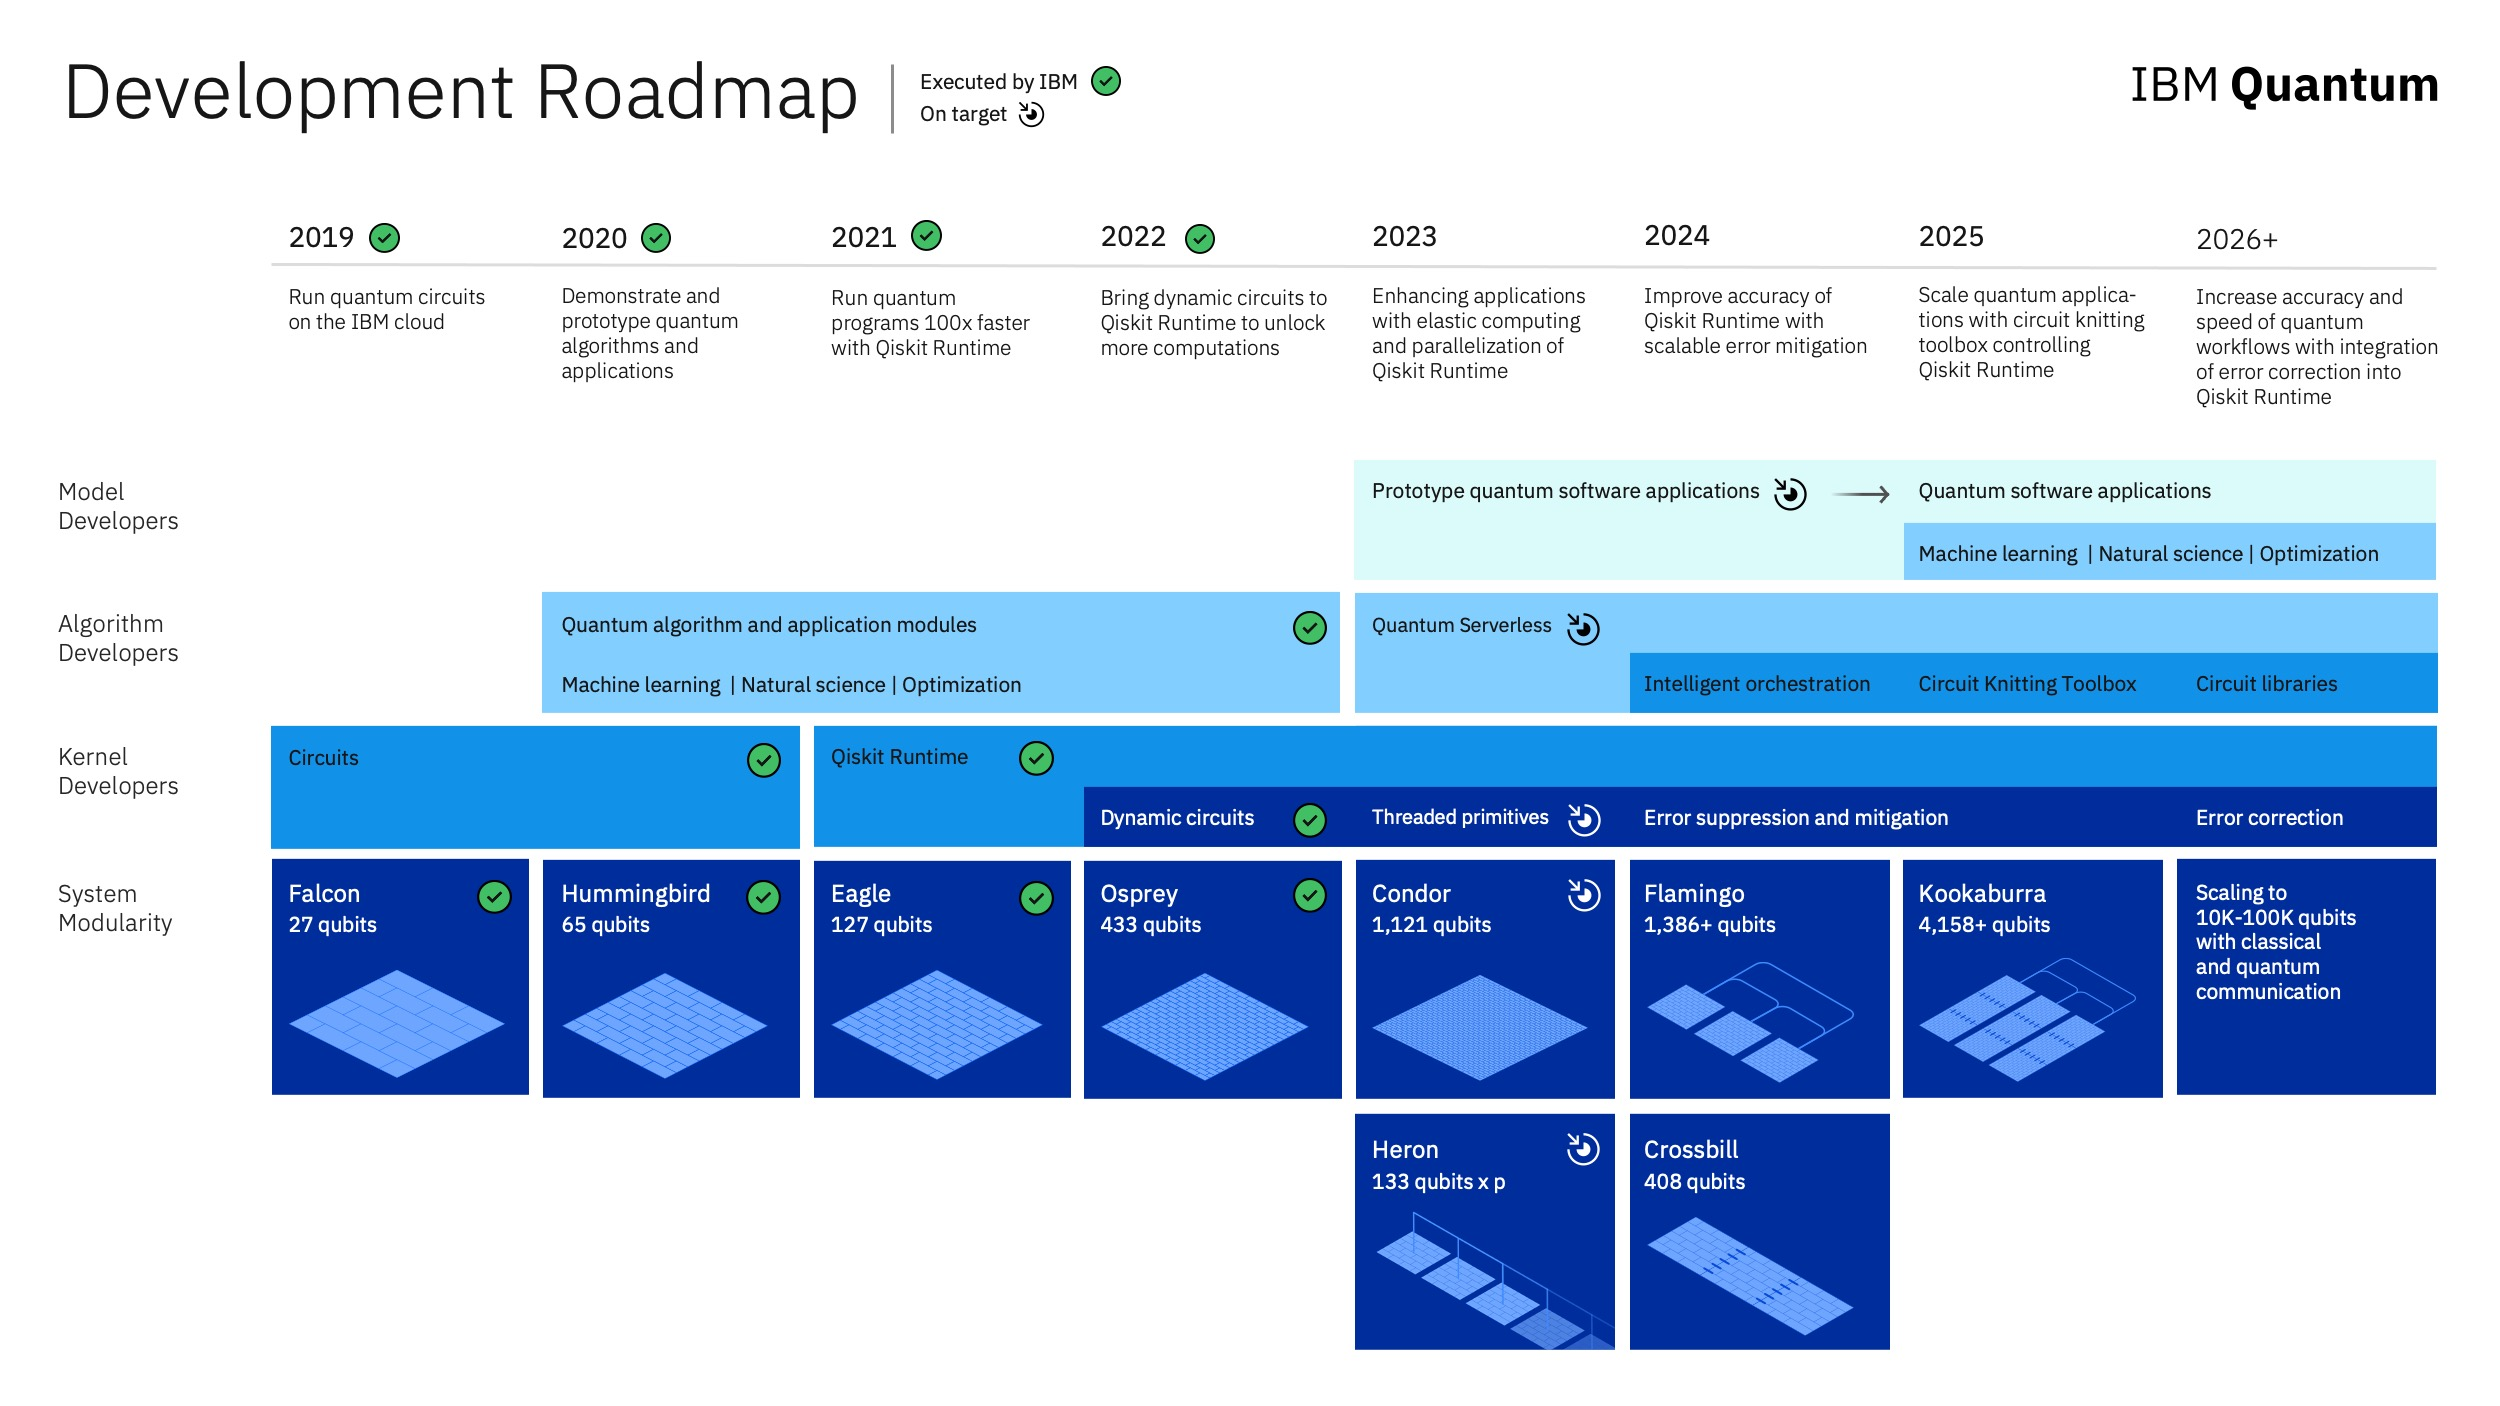
\includegraphics[width=\columnwidth]{IBM-Quantum-DevRoadmap2022_Light.jpeg}
\centering
\end{figure}

In Anbetracht zukünftiger Entwicklungen haben Unternehmen wie Google, IBM und Microsoft umfangreiche Pläne zur Erweiterung ihrer Quantencomputing-Kapazitäten. 
Google plant beispielsweise die Errichtung eines Quanten-Campus, der bis 2030 über einen Quantencomputer mit einer Million Qubits verfügen soll~\cite{Google_2023}. 
Microsoft verfolgen ähnliche Ziele, wobei der konkrete Umfang ihrer Projekte bislang nicht öffentlich spezifiziert wurde.
Des weiteren erwartet das Bundesamt für Sicherheit in der Informationstechnik die Existenz kryptografisch relevanter Quantencomputer zu Beginn der 2030er Jahre~\cite{BSI_KPMG_2023}. 

\subsection{Vorteile gegenüber klassischen Rechnern} 
Quantenparallelismus 

\section{Fundament}
\subsection{Literatur} 
\subsubsection*{Shor's Algorithmus}
Der Algorithmus wurde erstmals in der Publikation \textit{"`Algorithms for Quantum Computation: Discrete Logarithms and Factoring"'} von Peter W. Shor veröffentlicht.

Die Arbeit von Shor umfasste zwei Algorithmen.
Der erste Algorithmus ermöglicht die effiziente Berechnung der Primfaktorzerlegung, 
während der zweite Algorithmus die effiziente Berechnung des diskreten Logarithmus ermöglicht.
Aufgrund ihrer konzeptionellen Ähnlichkeiten werden beide Algorithmen häufig kollektiv als "`Shor's Algorithmus"' bezeichnet.

Die Quantenberechnungen beider Algorithmen basieren auf arithmetische Operationen in Restklassen und der Quanten-Fourier-Transformation.
Da Shor die Umsetzung von arithmetischen Operationen in Restklassen sowie die Quanten-Fourier-Transformation nicht explizit behandelt,
stützt sich die Implementierung auf den Ergebnissen weiterer Arbeiten. 
Diese untersuchen insbesondere effiziente Methoden zur Durchführung von arithmetischer Operationen in Restklassen innerhalb eines Quantenschaltkreises.
Einige dieser Arbeiten untersuchen die Quanten-Fourier-Transformation, 
da diese ein notwendiges Element für gewisse Berechnungen darstellt.

In der Publikation \textit{"`Quantum Networks for Elementary Arithmetic Operations"'} erklären Vlatko Vedral,  Adriano Barenco und Artur Ekert,
wie die modulare Exponentiation in einem Quantenschaltkreis berechnet werden kann. 

St\'{e}phane Beauregard baut auf den Erkenntnissen von Vedral, Barenco und Ekert auf und
verbessert den Quantenschaltkreis für die arithmetische Operation der modularen Exponentiation.
Hierfür ersetzt Beauregard einen Teil des ursprünglichen Quantenschaltkreis,
der in der modularen Exponentiation für die Berechnung der Addition genutzt wurde, 
durch einen effizienteren Quantenschaltkreis,
wie ihn Thomas G. Draper in \textit{"`Addition on a Quantum Computer"'} beschreibt.
Des weiteren verwendet Beauregard diese Optimierungen in seiner Arbeit \textit{"`Circuit for Shor’s algorithm using 2n+3 qubits"'},
um eine Realisierung von Shor's Algorithmus zur Faktorisierung zu beschreiben.

Andere Arbeiten, die sich mit der Implementierung von Shors's Algorithmus auseinandersetzen,
realisieren die modularen Exponentiation, 
indem klassische Schaltkreise identisch in den Quantenkontext übersetzt werden.
Der Nachbau von klassischen Operationen ist aufgrund der unitären Natur von Quantenoperationen nicht die effizienteste Realisierung.
Des Weiteren meiden andere Arbeiten die Realisierung der modularen Exponentiation für allgemeine Eingaben. 
Ohne modulare Exponentiation sind diese Varianten nicht in der Lage die Berechnung variabler Werte zu verarbeiten.
Stattdessen dienen diese ausschließlich der Demonstration der Funktionsweise von Shor's Algorithmus und
sind nur in der Lage, ausgewählte Eingaben zu verarbeiten.

Bei Recherchen wurde keine allgemeine Variante gefunden,
die weniger Qubits benötigt als die Variante aus der Arbeit \textit{"`Circuit for Shor’s algorithm using 2n+3 qubits"'},
deswegen bildet diese die Grundlage der Implementierung ab.

















\section{Grundlagen}
In diesem Abschnitt werden einige grundlegende Elemente erläutert, 
die für das Verständnis der Funktionsweise des Shor-Algorithmus erforderlich sind.
Als Fundament sind Kenntnisse in der Modulararithmetik, lineare Algebra und den komplexen Zahlen Vorraussetzung. 

Vorkenntnisse über die Grundprinzipien der Quantenmechanik sind hilfreich, 
werden aber im folgenden Abschnitt erläutert. 


\subsection{RSA-Verschlüsselung}
Das RSA-Verfahren ist ein weitverbreitetes asymmetrisches Kryptosystem, 
das 1977 von Ron \textbf{R}ivest, Adi \textbf{S}hamir und Leonard \textbf{A}dleman entwickelt wurde~\cite{10.1145/359340.359342}. 
In asymmetrischen Verschlüsselungsverfahren werden zwei verschiedene Schlüssel verwendet: 
Ein öffentlicher Schlüssel zum Verschlüsseln von Nachrichten und ein privater Schlüssel zum Entschlüsseln dieser Nachrichten.
Der private Schlüssel kann auch dazu verwendet werden, 
Nachrichten zu verschlüsseln und 
die Verschlüsselung signiert praktisch die Nachrichten 
(streng genommen den Hash dieser Nachrichten, jedoch wird dies hier der Einfachheit halber nicht vertieft).
Eine Signatur kann mit dem öffentlichen Schlüssel bestätigt werden, 
damit kann der Nutzer des öffentlichen Schlüssels die Authentizität der Nachricht kontrollieren.

\subsubsection*{Funktionsweise}
Die Grundlage des RSA-Verfahrens basiert auf der Schwierigkeit, 
das Produkt zweier großer Primzahlen zu zerlegen. 

Zunächst wählt man zwei große Primzahlen \(p\) und \(q\) und 
berechnet deren Produkt: 
\[N = p \cdot q \text{ und } f=(p-1)(q-1)\]  
Nun wird der Exponent \(e\) teilerfremd zu \(f\) gewählt.
Darauf basierend wird der private Schlüssel \(d\) als das multiplikative Inverse von \(e\) modulo \(f\) berechnet.
Der öffentliche Schlüssel besteht aus \(N\) und dem Exponenten \(e\). 
Der private Schlüssel ist \(d\).

Eine zu sendende Nachricht \( M \) wird in einen numerischen Wert umgewandelt und mittels des öffentlichen Schlüssels verschlüsselt:
\[
  C = M^e \bmod N
\]
Der Empfänger kann die verschlüsselte Nachricht \(C\) dann mit seinem privaten Schlüssel entschlüsseln:
\[
  M = C^d \bmod N
\]

Eine Nachricht \( M \) kann als \(S\) mit dem privaten Schlüssel signiert werden:
\[
  S = M^d \bmod N
\]
Für die Verifikation der Nachricht \(M\) muss dem Nutzer des öffentlichen Schlüssels \(M\) bekannt sein. 
Die Signatur \(S\) sollte die Nachricht wiedergeben:
\[
  M = S^e \bmod N
\]

Der private Schlüssel kann kompromittiert werden, wenn es gelingt, die beiden Faktoren \(p\) und 
\(q\) aus dem öffentlichen Schlüssel \(N\) zu extrahieren. 
In diesem Fall wäre es möglich, den privaten Schlüssel zu berechnen. 
Dies würde es ermöglichen, sowohl verschlüsselte Nachrichten zu lesen als auch Nachrichten zu signieren, 
ohne ursprünglich im Besitz des privaten Schlüssels zu sein.

\subsubsection*{Schwierigkeiten für klassische Computer}
Ein klassischer Computer hat Schwierigkeiten, 
RSA-Verschlüsselung effizient zu brechen, 
da das Problem der Zerlegung einer Zahl \(N\) in seine Primfaktoren für große Zahlen exponentiell schwieriger wird. 
Nach dem aktuellen Stand (Herbst 2023~\cite{Hoever2022Krypto}) benötigen die besten klassischen Algorithmen exponentiell mehr Zeit zur Entschlüsselung, 
je länger der verwendete Schlüssel ist.
Daher wird RSA als sicher angesehen, solange die Schlüssellänge ausreichend groß ist.



\subsection{Qubits} 
\begin{quote}
  \noindent
  \textit{"`Der Anfang enthält also beides, Sein und
  Nichts; ist die Einheit von Sein und Nichts,
  -- oder ist Nichtsein, das zugleich Sein, und
  Sein, das zugleich Nichtsein ist."' \\
  --- Georg Wilhelm Friedrich Hegel}
\end{quote}

Die Repräsentation und Speicherung von Information ist ein zentraler Aspekt aller Computer, 
unabhängig von der verwendeten Technologie oder Architektur.
Heutzutage basieren klassische Computer in der Regel auf dem Binärsystem. 
In der klassischen Repräsentation ist das Bit die kleinste Informationseinheit, 
die eine von zwei mögliche Zustände annehmen kann: 0 oder 1. 
Ein Bit hat zu jedem Zeitpunkt einen klar definierten Zustand. 
Mehrmaliges Auslesen eines Bits führt zu keiner Zustandsänderung, 
sofern keine Operationen zwischen den Auslesungen durchgeführt werden.

Im Gegensatz dazu funktionieren Quantencomputer grundlegend anders. 
Sie stützen sich auf die Prinzipien der Quantenmechanik und 
verwenden anstelle von Bits sogenannte Quantenbits beziehungsweise Qubits zur Informationsrepräsentation. 
Ein einzelnes Qubit stellt die kleinstmögliche Informationseinheit dar, 
über die ein Quantencomputer verfügt.

Um die quantenmechanischen Zustände von Qubits zu beschreiben, 
wird die Dirac-Notation als mathematische Schreibweise genutzt~\cite{dirac_1939}.

Ein Qubit kann einen der beiden Basiszustände annehmen 0 oder  1:
\begin{center}
\(\ket{0}\) oder entsprechend \(\ket{1}\)
\end{center}

Des Weiteren kann ein Qubit auch beide der Basiszustände gleichzeitig einnehmen:
\begin{center}
\(\ket{\Psi} = \alpha\ket{0} + \beta\ket{1}\)
\end{center}
Dieses Phänomen ist eine der charakteristischen Eigenschaften von Qubits und wird als \emph{Superposition} bezeichnet.
Dabei handelt es sich bei den Vorfaktoren \(\alpha\) und \(\beta\) um rationale Zahlen, 
für die gilt:
\begin{center}
\(\lvert\alpha\rvert^2 + \lvert\beta\rvert^2 = 1\)
\end{center} 


Es gibt unendlich viele Zustände, die ein Qubit in einer Superposition der beiden Basiszustände annehmen kann.

In der klassischen Welt findet man nur schwer eine Analogie zur Superposition. 
Man kann sich dies jedoch in etwa an einer Münze vorstellen~\cite{Hoever2023Münze}:

Ein klassisches Bit kann dabei entweder auf der Kopf- oder auf der Zahl-Seite liegen.
Ein Qubit hingegen ist eine Münze, 
die auf der Kante um die eigene Achse rotiert.
Dabei geben die Vorfaktoren \(\alpha\) und \(\beta\) an, 
wie die Münze zu der einen oder zu der anderen Seite tendiert.

Um ein Ergebnis zu erhalten, 
muss das Qubit gelesen werden, 
beziehungsweise genauer gesagt, gemessen.
Durch die Messung wird die Superposition zerstört und 
das Qubit kollabiert in einen der beiden Basiszustände.

In Analogie zur Münze wird die Rotation der Münze gezielt gestoppt, sodass diese auf eine der beiden Seiten kippt. 

Die Vorfaktoren \(\alpha\) und \(\beta\) repräsentieren die Amplituden des Qubits.
Die Amplituden beschreiben, 
wie stark die Tendenz des Qubits zu den Basiszuständen ist.
Bei einer Messung bestimmt die Tendenz die Wahrscheinlichkeit, 
in welchen der beiden Basiszustand das Qubit kollabieren.
Um die konkreten Wahrscheinlichkeiten für diese Zustände zu bestimmen, 
verwendet man die quadrierten Beträge der jeweiligen Vorfaktoren:
\begin{center}
\(\lvert\alpha\rvert^2\) für \(\ket{0}\), \(\lvert\beta\rvert^2\) für \(\ket{1}\)
\end{center}

Es ist nicht möglich, 
den Zustand eines Qubit während einer Berechnung zu beobachten,
da ansonsten die Superposition zerstört wird und in einen der beiden Basiszustände kollabiert.
Aus diesem Grund erfolgt die Messung in der Regel erst am Ende eines Quantenalgorithmus, um das endgültige Ergebnis zu ermitteln.

\bigskip

Qubits können über eine komplexe Phasenverschiebung verfügen:
\begin{center}
  \(
    \ket{\Psi} = (\alpha \cdot e^{i\varphi_1}) \cdot \ket{0} + (\beta \cdot e^{i\varphi_2}) \cdot \ket{1}
    \text{, }~
    \varphi_1,\varphi_2~\in~\mathbb{C}
  \)
  \end{center}
Wenn die komplexe Phasenverschiebung für beide Amplituden beziehungsweise Vorfaktoren identisch ist, 
spricht man von einer globalen Phase:
\begin{center}
  \(
    \ket{\Psi} = e^{i\varphi} \cdot (\alpha \ket{0} + \beta  \ket{1} )
    \text{, }~
    \varphi~\in~\mathbb{C}
  \)
\end{center}
Unterscheiden sich wiederum die Phasenverschiebung beider Vorfaktoren, 
handelt es sich um eine relative Phase:
\begin{center}
  \(
    \ket{\Psi} = (\alpha \cdot e^{i\varphi_1}) \cdot \ket{0} + (\beta \cdot e^{i\varphi_2}) \cdot \ket{1}
    \text{, }~
    \varphi_1,\varphi_2~\in~\mathbb{C}
    \text{, }~
    \varphi_1 \neq \varphi_2
  \)
\end{center}
Phasenverschiebungen können während einer Berechnung Zwischenergebnisse beeinflussen. 
Bei einer Messung hingegen hat eine Phasenverschiebung keinen Einfluss auf das Messergebnis, 
da nur die Betragsquadrate ausschlaggebend sind~\cite{Hoever2023QC}. 

\bigskip

In Rechnungen wird häufig die vektorielle Darstellung genutzt, 
um ein Qubit darzustellen. 
Für die beiden Basiszustände gilt:
\[
  \ket{0} = 
  \begin{pmatrix}
    1 \\
    0
  \end{pmatrix},~ 
  \ket{1} = 
  \begin{pmatrix}
    0 \\
    1
  \end{pmatrix}
  \]
oder im Allgemeinen:
\[
  \ket{\Psi} 
  =
  (\alpha \cdot e^{i\varphi_1}) \cdot \ket{0} + (\beta \cdot e^{i\varphi_2}) \cdot \ket{1}
  =  
  (\alpha \cdot e^{i\varphi_1}) \cdot 
  \begin{pmatrix}
    1 \\
    0
  \end{pmatrix} + (\beta \cdot e^{i\varphi_2}) \cdot 
  \begin{pmatrix}
    0 \\
    1
  \end{pmatrix} 
  =
  \begin{pmatrix}
    \alpha \cdot e^{i\varphi_1} \\
    \beta \cdot e^{i\varphi_2}
  \end{pmatrix}
\] 

\subsection{Quantengatter}
Während ein klassischer Rechner logische Gatter wie AND, OR und NOT nutzt um Bits zu manipulieren, 
verwendet ein Quantencomputer Quantengatter, 
um die Zustände von Qubits zu steuern. 
Im Gegensatz zu klassischen logischen Gattern führen Quantengatter stets unitäre Transformationen durch. 
Das bedeutet, dass die durch das Quantengatter bewirkte Änderung reversibel ist und 
die Norm des Zustandsvektors bewahrt. 
Somit wird die grundlegende Bedingung eines Qubits nicht verletzt:
\begin{center}
\(\lvert\alpha\rvert^2 + \lvert\beta\rvert^2 = 1\)
\end{center}
Des Weiteren haben Quantengatter die identische Anzahl an Ausgangsqubits wie Eingangsqubit, 
andernfalls würde dies ebenfalls keine unitäre Transformation darstellen.

Im Verlauf dieser Arbeit werden insbesondere Pauli-X-Gatter, Hadamard-Gatter und Phasen-Gatter verwendet. 
Die Transformationen dieser Gatter werden in Form einer Matrix beschrieben.

\subsubsection*{Pauli-X-Gatter}
Das Pauli-X-Gatter oder auch X-Gatter und Not-Gatter genannt, 
wirkt die Transformation: 
\[
  X = 
  \begin{pmatrix}
    0 & 1 \\
    1 & 0
    \end{pmatrix}
  \]
Die Wirkung auf Qubits in den Basiszuständen ähnelt dem logischen Not, 
daher kommt auch die Bezeichnung als Not-Gatter:
\begin{align*}
  &X \cdot
  \ket{0} 
  =
  \begin{pmatrix}
    0 & 1 \\
    1 & 0
    \end{pmatrix}
    \cdot
    \begin{pmatrix}
      1 \\
      0
    \end{pmatrix}
    = 
    \begin{pmatrix}
      0 \\
      1
    \end{pmatrix}
    = 
    \ket{1}
    \text{ bzw.} \\
    &X \cdot
  \ket{1} 
  =
  \begin{pmatrix}
    0 & 1 \\
    1 & 0
    \end{pmatrix}
    \cdot
    \begin{pmatrix}
      0 \\
      1
    \end{pmatrix}
    = 
    \begin{pmatrix}
      1 \\
      0
    \end{pmatrix}
    = 
    \ket{0}
  \end{align*}
Im Allgemeinen führt das Pauli-X-Gatter einen Bitflip durch, 
indem die Vorfaktoren vertauscht werden:
\[
  \begin{pmatrix}
    0 & 1 \\
    1 & 0
    \end{pmatrix}
    \cdot
    \begin{pmatrix}
      \alpha \\
      \beta
    \end{pmatrix}
    =
    \begin{pmatrix}
      \beta \\
      \alpha
    \end{pmatrix}
  \]


\subsubsection*{Hadamard-Gatter}
Das Hadamard-Gatter realisiert die Transformation:
\[
  H 
  =
  \frac{1}{\sqrt{2}}
  \begin{pmatrix}
    1 & 1 \\
    1 & -1
    \end{pmatrix}
\]
Die Zustände \(\ket{0}\) und \(\ket{1}\) sind die Basiszustände der sogenannten Standardbasis.
Wendet man auf \(\ket{0}\) und \(\ket{1}\) die Hadamard-Transformation an, 
werden diese entsprechend zu den Basiszuständen der Fourierbasis \(\ket{+}\) und \(\ket{-}\):
\begin{align*} 
  &\frac{1}{\sqrt{2}}
\begin{pmatrix}
  1 & 1 \\
  1 & -1
  \end{pmatrix}
  \cdot
  \begin{pmatrix}
    1 \\
    0
  \end{pmatrix}
  =
  \frac{1}{\sqrt{2}}
  \begin{pmatrix}
    1 \\
    1
  \end{pmatrix}
  =
  \ket{+}
  \quad\text{ und } \\
  &\frac{1}{\sqrt{2}}
  \begin{pmatrix}
    1 & 1 \\
    1 & -1
    \end{pmatrix}
    \cdot
    \begin{pmatrix}
      0 \\
      1
    \end{pmatrix}
    =
    \frac{1}{\sqrt{2}}
    \begin{pmatrix}
      1 \\
      -1
    \end{pmatrix}
    =
    \ket{-}
  \end{align*}
  Zustände in der Fourierbasis, einschließlich der beiden Basiszustände, unterscheiden sich lediglich durch ihre relative Phase:
\begin{align*}
  \ket{-} =
  \frac{1}{\sqrt{2}}
  \begin{pmatrix}
    1 \\
   - 1
  \end{pmatrix} &= 
  \frac{1}{\sqrt{2}}
  \begin{pmatrix}
    1 \\
   e^{\pi i} \cdot 1
  \end{pmatrix} \\ &= 
  \frac{1}{\sqrt{2}}
  \begin{pmatrix}
    1 & 0 \\
    0 & e^{\pi i}
  \end{pmatrix}
  \begin{pmatrix}
    1 \\
    1
  \end{pmatrix} = 
  \begin{pmatrix}
    1 & 0 \\
    0 & e^{\pi i}
  \end{pmatrix}
  \ket{+}
  \end{align*}

Wendet man die Transformation des Hadamard-Gatters auf die Basiszustände der Fourierbasis an, 
wird deutlich,
dass die Hadamard-Transformation von einer Phase beeinflusst wird:
\begin{align*}
  H \cdot \ket{+} &=
  \frac{1}{\sqrt{2}}
  \begin{pmatrix}
    1 & 1 \\
    1 & -1
  \end{pmatrix}
  \cdot
  \frac{1}{\sqrt{2}}
  \begin{pmatrix}
    1 \\
    1
  \end{pmatrix}
  =
  \begin{pmatrix}
    1 \\
    0
  \end{pmatrix}
  =
  \ket{0}\\
  H \cdot \ket{-} &=
  \frac{1}{\sqrt{2}}
  \begin{pmatrix}
    1 & 1 \\
    1 & -1
  \end{pmatrix}
  \cdot
  \frac{1}{\sqrt{2}}
  \begin{pmatrix}
    1 \\
    -1
  \end{pmatrix}
  =
  \begin{pmatrix}
    0 \\
    1
  \end{pmatrix}
  =
  \ket{1}
\end{align*}


Im Kapitel der Quanten-Fourier-Transformation~\ref{Quanten-Fourier-Transformation} wird dies vertieft.
Für ein besseres Verständnis dieses Kapitels ist es hilfreich, 
im Hinterkopf zu behalten, 
dass das Ergebnis eines Hadamard-Gatters von der Phasenverschiebung des Zustandes beeinflusst wird.


\subsubsection*{Phase-Gatter}
Das Phase-Gatter realisiert die Transformation:
\[
  P(\lambda) =
  \begin{pmatrix}
    1 & 0 \\
    0 & e^{i\lambda}
    \end{pmatrix}
  \]
Damit fügt das Phase-Gatter eine Phasenverschiebung zum \(\ket{1}\)-Anteil eines Qubits hinzu:
\[
  \begin{pmatrix}
    1 & 0 \\
    0 & e^{i\lambda}
    \end{pmatrix}
    \cdot
    \begin{pmatrix}
      \alpha \\
      \beta
    \end{pmatrix}
      =
    \begin{pmatrix}
      \alpha \\
      e^{i\lambda} \cdot \beta
    \end{pmatrix}
\]


\subsubsection*{Kontrollierte Gatter}
Ein weiterer wichtiger Baustein sind die kontrollierten Gatter. 
Kontrollierte Gatter werden durch ein Qubit kontrolliert und wirken auf mindestens ein anderes Qubit. 
Beachtet man die Basiszustände, 
so wird die Transformation nur ausgeführt, 
wenn das Kontroll-Qubit im Zustand \(\ket{1}\) ist.

Als Beispiel wird der Effekt eines kontrollierten Pauli-X-Gatters beziehungsweise 
Controlled-Not-Gatters für die beiden Basiszustände betrachtet.
Der Quantenschaltkreis für die beiden Qubits \(\ket{x}\) und \(\ket{y}\), zusammengefasst \(\ket{xy}\), 
ist in Abbildung~\ref{fig:cnot} abgebildet.
Dabei handelt es sich bei \(\ket{x}\) um das Kontroll-Qubit und bei \(\ket{y}\) um das Ziel-Qubit:
\[\ket{00}\shortrightarrow\ket{00},~\ket{01}\shortrightarrow\ket{01},~
\ket{10}\shortrightarrow\ket{11},~\ket{11}\shortrightarrow\ket{10}
  \]
Also wird die Not-Transformation auf das Qubit \(\ket{y}\) nur ausgeführt, 
wenn das Qubit \(\ket{x}\) dem Zustand \(\ket{1}\) entspricht.
\begin{figure}[H]
  \centering
  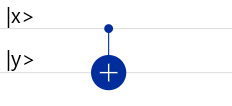
\includegraphics[scale=1]{cnot.png}
  \caption{CNot-Gatter}
  \label{fig:cnot}
\end{figure}

Im Verlauf dieser Arbeit werden einige kontrollierte Operationen verwendet. 
Für ein besseres Verständnis ist es hilfreich, 
sich diese Operationen mathematisch anzuschauen.
Die Transformation eines kontrollierten Pauli-X-Gatters lässt sich mit der folgenden Matrix beschreiben:
\[
  CX = 
  \begin{pmatrix}
    1 & 0 & 0 & 0\\
    0 & 1 & 0 & 0\\
    0 & 0 & 0 & 1\\
    0 & 0 & 1 & 0
    \end{pmatrix}
  \]
Um die Matrix mit den beiden Vektoren der beiden Qubits verrechnen zu können, 
wird das Tensorprodukt gebildet. Beispielsweise für \(\ket{xy}\) = \(\ket{10}\):
\[
  \begin{pmatrix}
    1 & 0 & 0 & 0\\
    0 & 1 & 0 & 0\\
    0 & 0 & 0 & 1\\
    0 & 0 & 1 & 0
    \end{pmatrix}
    \cdot
    \Bigg(
  \begin{pmatrix}
    0 \\
    1
  \end{pmatrix} \tensor
  \begin{pmatrix}
    1 \\
    0
  \end{pmatrix}
  \Bigg)
  =
  \begin{pmatrix}
    1 & 0 & 0 & 0\\
    0 & 1 & 0 & 0\\
    0 & 0 & 0 & 1\\
    0 & 0 & 1 & 0
    \end{pmatrix}
    \cdot
  \begin{pmatrix}
    0 \\
    0 \\
    1 \\
    0
  \end{pmatrix}
  =
  \begin{pmatrix}
    0 \\
    0 \\
    0 \\
    1
  \end{pmatrix}
  =
  \Bigg(
    \begin{pmatrix}
      0 \\
      1
    \end{pmatrix} \tensor
    \begin{pmatrix}
      0 \\
      1
    \end{pmatrix}
    \Bigg)
\]

Im Allgemeinen kann jedes Quanten-Gatter \(U\) als kontrolliertes Gatter eingesetzt werden. 
Dieses realisiert die Transformation~\cite{Hoever2023QC}: 
\[
  \text{für }
  U = 
  \begin{pmatrix}
    u_{00} & u_{01}\\
    u_{10} & u_{11}
    \end{pmatrix}
    \text{dementsprechend: }
    CU = 
  \begin{pmatrix}
    1 & 0 & 0 & 0\\
    0 & 1 & 0 & 0\\
    0 & 0 & u_{00} & u_{01}\\
    0 & 0 & u_{10} & u_{11}
    \end{pmatrix}
  \]


\subsubsection*{Aufeinander folgende Gatter} 

Um die Wirkung mehrerer Gatter zu berechnen, die nacheinander auf ein Qubit wirken, 
werden die Matrizen der Gatter in umgekehrter Reihenfolge aufgeschrieben, 
als diese im Quantenschaltkreis vorkommen. 
In Abbildung~\ref{fig:gate_order} wirkt zuerst ein Pauli-X-Gatter und anschließend ein Hadamard-Gatter auf das Qubit im Zustand \(\ket{0}\).
\[
  \frac{1}{\sqrt{2}}
  \begin{pmatrix}
    1 & 1 \\
    1 & -1
    \end{pmatrix} 
    \cdot
    \begin{pmatrix}
      0 & 1 \\
      1 & 0
      \end{pmatrix} 
    \cdot
    \begin{pmatrix}
      1  \\
      0 
      \end{pmatrix} 
      =
      \frac{1}{\sqrt{2}}
      \begin{pmatrix}
        1 & 1 \\
        1 & -1
        \end{pmatrix} 
      \cdot
      \begin{pmatrix}
        0  \\
        1 
        \end{pmatrix} 
        =
        \frac{1}{\sqrt{2}}
        \begin{pmatrix}
          1  \\
          -1 
          \end{pmatrix}
        =
        \ket{-}
  \]
\begin{figure}[H]
  \centering
  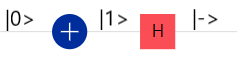
\includegraphics[scale=1]{gate_order.png}
  \caption{Berechnung aufeinanderfolgende Gatter}
  \label{fig:gate_order}
\end{figure}

\subsubsection*{Logische Gatter als Quantengatter} 
Das X-Gatter entspricht im Grunde genommen der identischen Transformation eines logischen NOT-Gatters für Basiszustände der Standardbasis.
\[
  X \cdot \ket{0} = \ket{1} 
  \text{ und }
  X \cdot \ket{1} = \ket{0}
\]
Quantengatter können die logischen Operatoren für zwei Bits, wie AND und XOR, 
nicht in ihrer herkömmlichen Form realisieren. 
Ein logisches AND als Quantengatter muss eines der beiden Qubits als Ergebnis der AND-Operation festlegen.
Im gegebenen Beispiel enthält das zweite Qubit das Ergebnis:
\[
  \ket{00} \shortrightarrow \ket{00} 
  \text{, } 
  \ket{01} \shortrightarrow \ket{00}
  \text{, }
  \ket{10} \shortrightarrow \ket{10}
  \text{, }
  \ket{11} \shortrightarrow \ket{11}
  \]
Unabhängig von der Definition des ersten Ausgangsqubits wird es immer zwei unterschiedliche Eingangszustände geben, 
die denselben Ausgangszustand haben. 

Es ist dennoch möglich, 
AND und OR als Quantengatter zu realisieren. 
Dafür muss ein Hilfsqubit verwendet werden, sodass das Quantengatter effektiv auf drei Qubits wirkt.

\subsection{Notation}
Die Notation von Quantenzuständen und Berechnungen ist in der Literatur nicht immer eindeutig. 
Um Mehrdeutigkeiten zu vermeiden, wird unter anderem die Schreibweise aus der Vorlesung "'Quanten Computing"` 
von Professor Hoever übernommen~\cite{Hoever2023QC}.

Dazu werden Qubits mit einem Index \(x\) versehen: \(\ket{\psi}_x\). 
Der Index gibt an, wie viele Qubits die Notation umfasst. 
Beispielsweise entspricht \(\ket{1}_1\) einem Qubit, 
welches sich im Zustand \(\ket{1}\) befindet.
Dank des Index ist bei den Qubits \(\ket{1}_3\) klar, 
dass es sich um drei Qubits handelt. 
Die Wertigkeit der Qubits wird durch die Reihenfolge festgelegt, 
dabei hat jedes Qubit den Wert einer Zweierpotenz.
Bei \(\ket{1}_3\) befinden sich die ersten beiden Qubits im Zustand \(\ket{0}\) und das Letzte im Zustand \(\ket{1}\).
Hingegen beschreibt \(\ket{4}_3\) ebenfalls drei Qubits, 
wobei diesmal das erste Qubit im Zustand \(\ket{1}\) ist und die letzten beiden dem Zustand \(\ket{0}\) entsprechen.
Also:
\[\ket{1}_3 = \ket{0}_1 \tensor \ket{0}_1 \tensor \ket{1}_1 = \ket{001}_3,~
\ket{4}_3 = \ket{1}_1 \tensor \ket{0}_1 \tensor \ket{0}_1 = \ket{100}_3\]

Ohne den Index 3 wäre die \(\ket{100}_3\) zweideutig. 
Der Index gibt an, dass es nur drei Qubits gibt. 
Da die dezimale 100 in binärer Schreibweise nicht mit drei Qubits darstellbar ist, 
muss es sich um die dezimale 4 handeln.

Zustände, die weder ein spezifisches Qubit noch ein Quantenregister beschreiben, 
werden ohne Index aufgeschrieben:
\[
  \ket{\psi}_1 = \alpha\ket{0} + \beta\ket{1}
  \]
Der Index wird auch ausgelassen, 
wenn ein Quantenregister einen Zustand beschreibt, 
der keine eindeutige Anzahl an Qubits vorschreibt.

\bigskip

Wenn mehrere gleiche Gatter parallel auf die identische Anzahl an Qubits angewendet werden 
oder das Gatter auf mehrere Qubits wirkt, 
wird das Gatter im Exponenten mit einem Tensor inklusive des Index beschrieben:
\[
  U^{\tensor x} \cdot 
  \ket{\psi}_x
\]


\subsection{Quanten-Fourier-Transformation} \label{Quanten-Fourier-Transformation}
Die Quanten-Fourier-Transformation bildet einen wesentlichen Bestandteil des implementierten Quantenalgorithmus. 
Im folgenden Abschnitt wird die allgemeine Anwendung der Quanten-Fourier-Transformation erklärt.
Darüber hinaus wird die Implementierung des Quantenschaltkreises anhand der Formel der Quanten-Fourier-Transformation hergeleitet.

Im Prinzip handelt es sich bei der Quanten-Fourier-Transformation um eine Transformation,
die Qubits von der Standardbasis (\(\ket{0}\), \(\ket{1}\)),
in die entsprechende Fourierbasis (\(\ket{+}\), \(\ket{-}\)) überführt~\cite[215]{homeister2023quantum215}.
Bei dem Basiswechsel werden die Informationen des vorherigen Zustands der Standardbasis in die Phase des neuen Zustandes übertragen~\cite{Ruiz-Perez2017}.
Anschließend können in der Fourierbasis Rechnungen durchgeführt werden, 
die im Grunde durch Manipulationen der Phase realisiert werden.
Mit diesem Ansatz ist es möglich, arithmetische Operationen, wie beispielsweise 
die Addition, effizienter zu berechnen~\cite{draper2000addition,Ruiz-Perez2017}.

Unter Verwendung der inversen Quanten-Fourier-Transformation, 
die als Rücktransformation dient, ist es möglich, 
wieder zurück in die Standardbasis zu transformieren. 
Dies ermöglicht die Extraktion der Information aus der Phase in einen messbaren Zustand.

Die Quanten-Fourier-Transformation ist für ein \(N\) = \(2^n\) mit \(n\) Qubits
für die Basisvektoren \(\ket{x}, x = 0,...,N-1\) wie folgt definiert~\cite[216]{homeister2023quantum215}:
\[QFT_{N}\ket{x}_{n} = \frac{1}{\sqrt{N}}\sum_{y=0}^{N-1}  e^{\frac{2 \pi i x y}{N}}\ket{y}_{n}\]
Anhand dieser Definition kann der Quantenschaltkreis nicht direkt hergeleitet werden.
Stattdessen muss die Formel umgeformt werden.

Die folgende Herleitung stammt aus dem Lehrbuch \textit{Quantum Computation and Quantum Information}~\cite[218]{nielsen_chuang_2010}.
Der Übersicht halber werden Zwischenschritte hinzugefügt.

Indem \(y\) in der ersten Formel in die Binärschreibweise überführt wird, ergibt sich:
\[ y = \sum_{k=1}^{n}2^{n-k} y_{n-k+1}\]  
\begin{align}
  QFT_{N}\ket{x}_{n} &=
    \frac{1}{\sqrt{N}}
    \sum_{y_n=0}^{1} ...
    \sum_{y_1=0}^{1} e^{\frac{2 \pi i x \sum_{k=1}^{n}2^{n-k} y_{n-k+1}}{N}}
    \ket{y_n ... y_{2}y_{1}}
\end{align}
Mit \(N\) = \(2^n\) kann der Bruch im Exponenten gekürzt werden:
\[QFT_{N}\ket{x}_{n} = \frac{1}{\sqrt{N}}\sum_{y_n=0}^{1}...\sum_{y_1=0}^{1}  e^{\frac{2 \pi i x \sum_{k=1}^{n}2^{n-k} y_{n-k+1}}{2^n}}\ket{y_n ... y_{2}y_{1}}\]
\[QFT_{N}\ket{x}_{n} = \frac{1}{\sqrt{N}}\sum_{y_n=0}^{1}...\sum_{y_1=0}^{1}  e^{2 \pi i x \sum_{k=1}^{n}2^{-k} y_{n-k+1}}\ket{y_n ... y_{2}y_{1}}\]
Anschließend kann der Ausdruck \(2^{-k}\) zu \(\frac{1}{2^k}\) umgeformt werden: 
\[QFT_{N}\ket{x}_{n} = \frac{1}{\sqrt{N}}\sum_{y_n=0}^{1}...\sum_{y_1=0}^{1}  e^{\frac{2 \pi i x \sum_{k=1}^{n} y_{n-k+1}}{2^k}}\ket{y_n ... y_{2}y_{1}}\]
Die Summe im Exponenten der Basis \(e\) kann als Produkt umgeschrieben werden.
Anstatt dem Produktzeichen \(\prod\) wird das Tensorprodukt \(\Tensor\) verwendet, da es sich um Qubits handelt:
\[QFT_{N}\ket{x}_{n} = \frac{1}{\sqrt{N}}\sum_{y_n=0}^{1}...\sum_{y_1=0}^{1} \Tensor_{k=1}^n{ e^{\frac{2 \pi i x y_k}{2^k}}}\ket{y_{k}}\]
Der Ausdruck kann weiter vereinfacht werden indem das Tensorprodukt vorgezogen wird:
\[QFT_{N}\ket{x}_{n} = \frac{1}{\sqrt{N}}\Tensor_{k=1}^n \Big[  \sum_{y_k=0}^{1}{ e^{\frac{2 \pi i x y_k}{2^k}}}\ket{y_{k}}\Big]\]
\[QFT_{N}\ket{x}_{n} = \frac{1}{\sqrt{N}}\Tensor_{k=1}^n \Big[  \ket{0} + { e^{\frac{2 \pi i x}{2^k}}}\ket{1}\Big]\] 
Schreibt man das Tensorprodukt voll aus und notiert \(x\) in Binärschreibweise, erhält man:
\begin{align*}
\frac{1}{\sqrt{N}}\Bigg(
  \Big(\ket{0} + { e^{\frac{2 \pi i (2^{n-1}x_n+...+2^1x_2+2^0x_1)}{2^1}}}\ket{1}\Big)
  &\tensor
  \Big(\ket{0} + { e^{\frac{2 \pi i (2^{n-1}x_n+...+2^1x_2+2^0x_1)}{2^2}}}\ket{1}\Big) \\
  &\vdotswithin{\tensor} \\
  &\tensor
  \Big(\ket{0} + { e^{\frac{2 \pi i (2^{n-1}x_n+...+2^1x_2+2^0x_1)}{2^n}}}\ket{1}\Big)
  \Bigg)
\end{align*}
Die komplexe Exponentialfunktion ergibt für eine natürliche Zahl \(k\): \(e^{2\pi i k} = 1\).
Mit dieser Eigenschaft kann man beispielsweise die Phasenverschiebung des ersten Tensors vereinfachen:
\begin{align*} 
  e^{\frac{2 \pi i (2^{n-1}x_n+ \dotsb +2^1x_2+2^0x_1)}{2^1}}
  &=
  e^{\frac{2 \pi i (2^{n-1}x_n)}{2^1}} \dotsb e^{\frac{2 \pi i (2^1x_2)}{2^1}} e^{\frac{2 \pi i (2^0x_1)}{2^1}} \\
  &=
  e^{{2 \pi i (2^{n-2}x_n)}} \dotsb e^{{2 \pi i (2^0x_2)}} e^{{2 \pi i (2^{-1}x_1)}}
\end{align*}
Dabei ergibt nur der Term \(e^{{2 \pi i (2^{-1}x_1)}} \neq 1 \)  
und verursacht somit eine relevante Phasenverschiebung.

Abschließend lässt sich das gesamte Tensorprodukt vereinfachen:
\begin{align*}
  QFT_{N}\ket{x}_{n} = 
  \frac{1}{\sqrt{N}}
  \Bigg(
    \Big(\ket{0} + { e^{\frac{2 \pi i (2^0x_1)}{2^1}}}\ket{1}\Big) 
    &\tensor
    \Big( \ket{0} + { e^{\frac{2 \pi i (2^1x_2+2^0x_1)}{2^2}}}\ket{1}\Big) \\
    &\vdotswithin{\tensor}\\
    &\tensor
    \Big( \ket{0} + { e^{\frac{2 \pi i (2^{n-1}x_n+ ... +2^1x_2+2^0x_1)}{2^n}}}\ket{1}\Big)
  \Bigg)
\end{align*}
Ein einzelner Tensor repräsentiert die Wirkung der Quantenschaltung auf ein einzelnes Qubit. 
Somit werden die Phasenverschiebungen erkennbar, 
die auf ein Qubit wirken. 
Außerdem verdeutlicht die Binärschreibweise, 
dass die angewendete Phasenverschiebung vom Zustand anderer Qubits abhängig sind.

Für die Implementierung der Quanten-Fourier-Transformation sind nur die Terme relevant, 
die eine Phasenverschiebung von ungleich 1 bewirken. 
Dies lässt sich mit der folgenden Formel beschreiben:
\[
QFT_{N}\ket{x}_{n} = \frac{1}{\sqrt{N}}
\Tensor_{k=1}^n \Big[  \ket{0} + { e^{\frac{2 \pi i \sum_{b=0}^{k-1}2^b x_{b+1} }{2^k}}}\ket{1}\Big]
\] 
Im Weiteren wird diese Formel verwendet, 
um einen Quantenschaltkreis für die Quanten-Fourier-Transformation mit drei Qubits zu implementieren:
\begin{align*}
QFT_{8}\ket{x}_{3} = 
\frac{1}{\sqrt{8}} 
  \Bigg[
    \Big(\ket{0} + { e^{\frac{2 \pi i (2^0x_1)}{2^1}}}\ket{1} \Big) 
    &\tensor
    \Big(\ket{0} + { e^{\frac{2 \pi i (2^1x_2+2^0x_1)}{2^2}}}\ket{1} \Big) \\
    &\tensor
    \Big(\ket{0} + { e^{\frac{2 \pi i (2^{2}x_3 +2^1x_2+2^0x_1)}{2^3}}}\ket{1} \Big) 
  \Bigg] 
\end{align*}
Man kann die durch den Eingangszustand eines einzelnen Qubits erzeugte Phasenverschiebung verdeutlichen, 
indem man die Addition im Exponenten zu einer Multiplikation der gleichen Basen umformt:
\begin{align*}
  QFT_{8}\ket{x}_{3} = 
  \frac{1}{\sqrt{8}} 
  \Bigg[
    \Big(\ket{0} + { e^{\frac{2 \pi i (2^0x_1)}{2^1}}}\ket{1}\Big) 
    &\tensor
    \Big(\ket{0} + { e^{\frac{2 \pi i (2^1x_2)}{2^2}} e^{\frac{2 \pi i (2^0x_1)}{2^2}} }\ket{1} \Big) \\ 
    &\tensor
    \Big(\ket{0} + { e^{\frac{2 \pi i (2^{2}x_3)}{2^3}} e^{\frac{2 \pi i (2^1x_2)}{2^3}} e^{\frac{2 \pi i (2^0x_1)}{2^3}}  }\ket{1} \Big)
  \Bigg] 
\end{align*}
Die wirkenden Phasenverschiebungen werden eindeutiger, 
indem man die Brüche kürzt:
\begin{align*}
  QFT_{8}\ket{x}_{3} = 
  \frac{1}{\sqrt{8}} 
  \Bigg[ 
    \Big( \ket{0} + e^{\pi i x_1}\ket{1} \Big) &\tensor
    \Big(\ket{0} + { e^{\pi i x_2} e^{ \frac{ \pi i x_1}{2}} }\ket{1} \Big) \\ &\tensor
    \Big(\ket{0} + { e^{\pi i x_3} e^{\frac{\pi i x_2}{2}} e^{ \frac{ \pi i x_1}{4}} }\ket{1} \Big) 
  \Bigg] 
\end{align*}
In einer abschließenden Umformung lässt sich der Bruch \(\frac{1}{\sqrt8}\) aufteilen.
Dadurch erinnern die einzelnen Tensoren,
beziehungsweise Qubits an die Form die durch eine Hadamard-Transformation entsteht:
\begin{align*}
  QFT_{8}\ket{x}_{3} = 
   \frac{1}{\sqrt{2}}\Big( \ket{0} + e^{\pi i x_1}\ket{1} \Big) 
   &\tensor
  \frac{1}{\sqrt{2}}\Big( \ket{0} + { e^{\pi i x_2} e^{ \frac{ \pi i x_1}{2}} }\ket{1} \Big) \\ 
  &\tensor
  \frac{1}{\sqrt{2}}\Big( \ket{0} + { e^{\pi i x_3} e^{\frac{\pi i x_2}{2}} e^{ \frac{ \pi i x_1}{4}} }\ket{1} \Big)  
\end{align*}
Die Phasenverschiebung \(e^{\pi i}\) ist in jedem der einzelnen Qubits vorhanden.
Des Weiteren ist diese Phasenverschiebung von dem Eingangszustand des Qubits abhängt,
auf das die Verschiebung auch angewendet wird. 
Konkret bedeutet dies, 
dass auf jedes Qubit in dem Zustand \(\ket{1}\) eine Phasenverschiebung von \(e^{\pi i}\) wirkt.
Anhand des ersten Qubits, 
beziehungsweise des ersten Tensors, 
ergibt sich bei \(x_1 = 0\)
der Zustand: 
\[\frac{1}{\sqrt{2}}(\ket{0} + e^{\pi i 0} \ket{1}) = \frac{1}{\sqrt{2}}(\ket{0} + \ket{1})\]
Bei \(x_1 = 1\) wird der Zustand zu:
\[\frac{1}{\sqrt{2}}(\ket{0} + e^{\pi i 1} \ket{1}) = \frac{1}{\sqrt{2}}(\ket{0} - \ket{1})\]
Aufgrund des Vorfaktors von \(\frac{1}{\sqrt{2}}\) entsprechen beide Fälle also der Hadamard"=Transformation.
Da alle anderen Tensoren ebenfalls den Ausdruck \(e^{\pi i x_k}\) 
und den Vorfaktor \(\frac{1}{\sqrt{2}}\) beinhalten, 
wirkt auf jedes Qubit ein Hadamard-Gatter.

Die weiteren Tensoren des Tensorprodukts beinhalten zunehmend mehr Ausdrücke, 
die für unterschiedliche Phasenverschiebungen sorgen. 
Die Phasenverschiebung eines einzelnen Ausdrucks kann mit einem Phasen-Gatter realisiert werden. 

Beispielsweise wirkt auf das zweite Qubit ein Phasen-Gatter mit \(P(\frac{\pi}{2} )\).
Diese Phasenverschiebung soll jedoch nur angewendet werden, 
wenn \(x_1 = 1\) ist.
Aus diesem Grund wird das Phasen-Gatter durch den Eingangszustand des ersten Qubits gesteuert und 
mithilfe eines kontrollierten Phasen-Gatters realisiert.
Das gleiche Prinzip gilt für alle weiteren Qubits.
Anschließend ergibt sich ein Quantenschaltkreis, 
wie dieser in Abbildung~\ref{fig:qft} dargestellt ist.

Wie in Abbildung~\ref{fig:qft} ersichtlich, 
kehrt die Quanten-Fourier-Transformation die Reihenfolge der Qubits um~\cite[217]{homeister2023quantum215}.
Um die ursprüngliche Reihenfolge wiederherzustellen, 
werden am Ende der Quanten-Fourier-Transformation Swap-Operationen durchgeführt.
\begin{figure}[H]
  \centering
  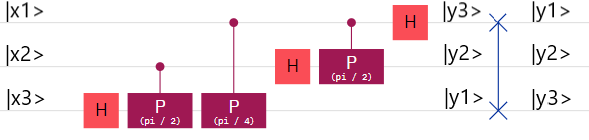
\includegraphics[width=\columnwidth]{qft.PNG}
  \caption{3-Qubit QFT}
  \label{fig:qft}
\end{figure}

Anhand der Implementierung wird ersichtlich,
dass die Quanten-Fourier-Transformation unitär ist. 
Diese Eigenschaft ergibt sich aus der Tatsache, 
dass der zugehörige Quantenschaltkreis ausschließlich unter Verwendung von unitären Gattern realisierbar ist.

Wie bereits oben erwähnt, 
wird für die Rücktransformation aus der Fourierbasis in die Standardbasis die inverse Quanten-Fourier-Transformation angewendet.
Um einen Quantenschaltkreis aus unitären Gattern zu invertieren, 
werden die Inversen der verwendeten Gatter in umgekehrter Reihenfolge zur ursprünglichen Schaltung angewendet. 
Die Swap-Operationen stehen somit bei der inversen Quanten-Fourier-Transformation am Anfang.
In Abbildung~\ref{fig:iqft} ist beispielhaft die inverse Quanten-Fourier-Transformation für drei Qubits abgebildet.
\begin{figure}[H]
  \centering
  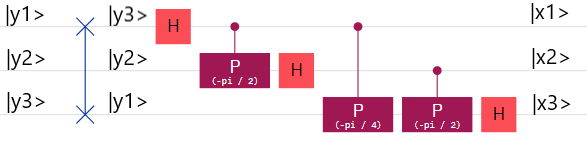
\includegraphics[width=\columnwidth]{iqft.PNG}
  \caption{3-Qubit inverse QFT}
  \label{fig:iqft}
\end{figure}

\subsection{Quantum-Phase-Estimation} \label{Quanten-Phase-Estimation}

Im nachfolgenden Abschnitt wird die Anwendung und Funktionsweise des Quantum-Phase-Estimation Quantenalgorithmus erläutert. 
Die Quantum-Phase-Estimation ist ein Bestandteil einiger fortgeschrittener Quantenalgorithmen und eine integrale Komponente des spezifischen Quantenalgorithmus, 
der in dieser Arbeit implementiert wird. 
Genauer gesagt, 
basiert der implementierte Quantenalgorithmus auf den Prinzipien der Quantum-Phase-Estimation und verwendet dieselbe Methodik für einen spezialisierten Kontext.

Schwerpunktmäßig konzentriert sich die Erklärung primär auf das Verständnis der Funktionsweise der Quantum-Phase-Estimation.
Die Anwendung der Quantum-Phase-Estimation benötigt ein paar Voraussetzungen die vom spezifischen Kontext abhängen, 
in dem die Quantum-Phase-Estimation angewendet wird.
Die Voraussetzungen werden für die Erklärung der Funktionsweise als Gegeben angesehen.

Im weiteren Verlauf der Arbeit werden diese Voraussetzungen im Hinblick auf den Anwendungsfall des implementierten Quantenalgorithmus konkretisiert.

Eine der Voraussetzungen ist, 
dass ein Eigenvektor \(\ket{x}_n\) einer unitären Transformation \(U^{\tensor n}\) bekannt ist.
Wendet man die Transformation \(U^{\tensor n}\) auf \(\ket{x}_n\) an, 
so gilt~\cite[221]{nielsen_chuang_2010}: 
\[U^{\tensor n}\ket{x}_n=\lambda_x\ket{x}_n\]
Dabei erhält man, abhängig vom gewählten Eigenvektor \(\ket{x}_n\), einen der Eigenwert \(\lambda_x\) von \(U^{\tensor n}\).
Ein Eigenwert \(\lambda_x\) besitzt die Form eines Phasenfaktors: \(e^{2\pi i \varphi_x}\),
mit \(0 \leq \varphi_x < 1\).
Im Prinzip wird durch die unitäre Transformation also eine globale Phasenverschiebung auf den Eigenvektor angewendet.

Wie bereits im Kapitel zu den Grundlagen gezeigt wurde, 
ist es nicht möglich, eine globale Phase durch eine gewöhnliche Messung der Qubits zu bestimmen. 
Das liegt daran, dass eine globale Phase die Amplituden eines Qubits nicht verändert und 
somit die Wahrscheinlichkeiten der Messergebnisse unverändert bleiben. 
Stattdessen muss man die Qubits so manipulieren, 
dass die globale Phase doch Einfluss auf die Amplituden nimmt.

Der Quantum-Phase-Estimation Quantenalgorithmus ist in der Lage, 
den Eigenwert aus \(U^{\tensor n}\ket{x}_n=\lambda_x\ket{x}_n\), 
also die Phasenverschiebungen repräsentiert durch \(\lambda_x = e^{2\pi i \varphi_x}\),
auf die Amplitude eines anderen Qubits zu verschieben.
Um \(\lambda_x\) auf ein anderes Qubit zu übertragen, 
wird der Effekt des \emph{Phase-Kickback} genutzt.
Anschließend wird der Wert \(\varphi_x\) des Eigenwertes durch die inverse Quanten-Fourier-Transformation in einen messbaren Zustand überführt.

Der Phase-Kickback tritt auf, 
wenn eine unitäre Transformation \(U^{\tensor n}\), die durch ein Qubit \(\ket{y}_1\) in Superposition kontrolliert wird,
auf einen Eigenvektor \(\ket{x}_n\) von \(U^{\tensor n}\) anwendet wird.
Dabei wird der Eigenwert, genauer gesagt \(\lambda_x\), 
auf den \(\ket{1}\)-Anteil von \(\ket{y}_1\) übertragen.

Sei \( \ket{y}_1 = \alpha\ket{0} + \beta\ket{1} \) mit \( \alpha,\beta \neq 0 \), dann gilt:
\begin{align*}
  CU^{\tensor n+1}(\ket{y}_1 \otimes \ket{x}_n) 
  &= CU^{\tensor n+1}\big((\alpha\ket{0} + \beta\ket{1}) \otimes \ket{x}_n\big) \\
  &= CU^{\tensor n+1}\big((\alpha\ket{0}\otimes\ket{x}_n) + (\beta\ket{1}\otimes \ket{x}_n)\big) \\
  &= \big((\alpha\ket{0}\otimes\ket{x}_n) + (\beta\ket{1}\otimes U^{\tensor n}\ket{x}_n)\big) \\
  &= \big((\alpha\ket{0}\otimes\ket{x}_n) + (\beta\ket{1}\otimes \lambda_x\ket{x}_n)\big) \\
  &= (\alpha\ket{0} + \lambda_x\beta\ket{1}) \otimes \ket{x}_n
\end{align*}
In der Rechnung wird also die globale Phase \(\lambda_x\) von \(\ket{x}_n\) als relative Phase auf \(\ket{y}_1\) übertragen.

Es folgt ein Beispiel welches den Effekt verdeutlicht:
Beachtet werden zwei Qubits im Zustand \(\ket{+}_1 \tensor \ket{-}_1\) auf die ein kontrolliertes X-Gatter angewendet wird.
Dabei ist \(\ket{-}_1\) der Eigenvektor einer X-Transformation mit zugehörigen Eigenwert \(e^{\pi i} = -1\), also: 
\[X \cdot \ket{-}_1=-\ket{-}_1\]
Auf das zweite Qubit \(\ket{-}_1\) wirkt ein \(CX^{\tensor 2}\) Gatter welches durch das erste Qubit \(\ket{+}_1\) kontrolliert wird:
\[
  CX^{\tensor 2}( \ket{+}_1\ \tensor \ket{-}_1) =
  \begin{pmatrix}
    1 & 0 & 0 & 0\\
    0 & 1 & 0 & 0\\
    0 & 0 & 0 & 1\\
    0 & 0 & 1 & 0
  \end{pmatrix}
  \cdot
  \frac{1}{{2}}
  \begin{pmatrix}
    1 \\
    -1 \\
    1 \\
    -1 
  \end{pmatrix}
  =
  \frac{1}{{2}}
  \begin{pmatrix}
    1 \\
    -1 \\
    -1 \\
    1 
  \end{pmatrix}
  \]
  \[
  =
  \frac{1}{{\sqrt{2}}}
  \begin{pmatrix}
    1 \\
    -1 
  \end{pmatrix}
  \tensor
  \frac{1}{{\sqrt{2}}}
  \begin{pmatrix}
    1 \\
    -1 
  \end{pmatrix}
  =
  \ket{-}_1 \tensor \ket{-}_1
  \]
Mit Hilfe des Phase-Kickback kann man also den Eigenwert einer unitären Transformation in die relative Phase eines Kontrollqubits verschieben.
Der Vorteil davon ist, 
dass diese Phasenverschiebung nur den Vorfaktor von \(\ket{1}\) des Kontrollqubits betrifft und keine globale Phase darstellt.

Der Aufbau einer Quantum-Phase-Estimation Quantenschaltung sieht beispielsweise wie folgt aus:
Beachtet wird die unitäre Transformation eines Phase-Gatters(P) mit einer variablen Phasenverschiebung von 
\[P(2 \pi \varphi ) = 
\begin{pmatrix}
  1 & 0\\
  0 & e^{2 i \pi \varphi}
\end{pmatrix}\]
Ein zugehöriger Eigenvektor dieser Transformation ist \(\ket{1}_1\), 
den: 
\[P(2 \pi \varphi)\ket{1}_1 = e^{2 i \pi \varphi} \ket{1}_1\]

Um den Effekt des Phase-Kickback nutzen zu können, 
muss sich das Kontrollqubit in einer Superposition befinden.
Dafür wird das Kontrollqubit im Zustand \(\ket{0}_1\) initialisiert und
anschließend mit einem Hadamard-Gatter(H) in die gleichmäßige Superposition \(\ket{+}_1\) versetzt.
\[\ket{0}_1 \tensor \ket{1}_1 
\underrightarrow{H^{\tensor 1}}
 \ket{+}_1 \tensor \ket{1}_1
=
\frac{1}{\sqrt{2}}
\begin{pmatrix}
  1 \\
  1
 \end{pmatrix}
 \tensor
 \begin{pmatrix}
  0 \\
  1 
 \end{pmatrix}
 =
 \frac{1}{\sqrt{2}}
 \begin{pmatrix}
  0 \\
  1 \\
  0 \\
  1
\end{pmatrix}
 \]
Über das kontrollierte Phase-Gatter wird der Eigenwert auf das Kontrollqubit verschoben und
befindet sich daher nicht mehr im Zustand \(\ket{+}_1\) :
\begin{align*}
  \frac{1}{\sqrt{2}}
  \begin{pmatrix}
   0 \\
   1 \\
   0 \\
   1
  \end{pmatrix}
  \underrightarrow{CP^{\tensor 2}(2 \pi \varphi)}
  \begin{pmatrix}
    1 & 0 & 0 & 0\\
    0 & 1 & 0 & 0\\
    0 & 0 & 1 & 0\\
    0 & 0 & 0 & e^{2 i \pi \varphi}
  \end{pmatrix}
  \cdot
  \frac{1}{\sqrt{2}}
  \begin{pmatrix}
   0 \\
   1 \\
   0 \\
   1
  \end{pmatrix}
  &=
  \frac{1}{\sqrt{2}}
  \begin{pmatrix}
    0 \\
    1 \\
    0 \\
    e^{2 i \pi \varphi}
  \end{pmatrix} \\
  &=
  \frac{1}{\sqrt{2}}
  \begin{pmatrix}
    1 \\
    e^{2 i \pi \varphi}
   \end{pmatrix}
   \tensor
   \begin{pmatrix}
    0 \\
    1 
   \end{pmatrix}
\end{align*}
Anschließend wird auf die Kontrollqubits die inverse Quanten-Fourier-Transformation angewendet.
Die inverse Quanten-Fourier-Transformation sorgt dafür, 
dass der Eigenwert die Amplituden der Kontrollqubits beeinflusst.
Die Qubits mit dem Eigenvektor sind für den weiteren Ablauf der Quantum-Phase-Estimation nicht mehr relevant 
und werden nicht weiter beachtet.
Im vorliegenden Beispiel entspricht die inverse Quanten-Fourier-Transformation einem einzelnen Hadamard-Gatter. 
Das liegt daran, dass lediglich ein Kontrollqubit vorhanden ist, 
auf das die inverse Quanten-Fourier-Transformation angewendet wird:
\[
\frac{1}{\sqrt{2}}
\begin{pmatrix}
  1 \\
  e^{2 i \pi \varphi}
 \end{pmatrix}
 \underrightarrow{H^{\tensor 1}}
 \frac{1}{\sqrt{2}}
 \begin{pmatrix}
  1 & 1\\
  1 & -1
 \end{pmatrix}
 \cdot
 \frac{1}{\sqrt{2}}
\begin{pmatrix}
  1 \\
  e^{2 i \pi \varphi}
 \end{pmatrix}
 =
 \frac{1}{2}
 \begin{pmatrix}
  1 + e^{2 i \pi \varphi}\\
  1 - e^{2 i \pi \varphi}
 \end{pmatrix}
\]
Das Ergebnis des Beispiels zeigt, dass der Eigenwert praktisch auf die Amplitude vom Kontrollqubit transformiert wird.

Verwendet man ein Phase-Gatter mit \(\varphi  = 0.075\), 
so sieht der Quantenschaltkreis wie in Abbildung~\ref{fig:qpe_1qubit} aus.
\begin{figure}[H]
  \centering
  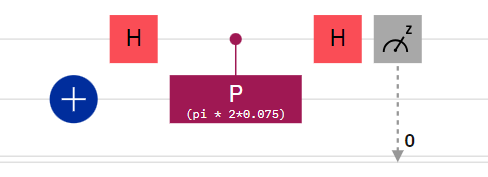
\includegraphics[ scale = 0.9]{qpe_1qubit.PNG}
  \caption{Einzelnes Kontroll-Qubit QPE}
  \label{fig:qpe_1qubit}
\end{figure}
Mit dieser Phasenverschiebung sollte man bei einer Messung den Zustand \(\ket{0}\)
mit einer Wahrscheinlichkeit von ungefähr \(0.9455\) 
und den Zustand \(\ket{1}\) mit der Wahrscheinlichkeit \(0.0544\) erhalten.
Die Ergebnisse von 20.000 Messungen, dargestellt in Abbildung~\ref{fig:qpe_1qubit_Messung}, 
bestätigen die Größenordnung dieser Wahrscheinlichkeiten.
Jedoch entsprechen die Messungen aus Abbildung~\ref{fig:qpe_1qubit_Messung} nicht ganz den theoretisch ausgerechneten Wahrscheinlichkeiten.
Dies liegt an der probabilistischen Natur der Messung.
Bei einer zunehmenden Anzahl an Messungen würden die Ergebnisse gegen die theoretisch erwarteten Wahrscheinlichkeitswerte konvergieren.
Somit sind viele Durchläufe des Quantenalgorithmus erforderlich, 
um anhand der Messungen ein verlässliches Ergebnis zu erhalten.
\begin{figure}[H]
  \caption{Einzelnes Kontroll-Qubit QPE Messung}
  \label{fig:qpe_1qubit_Messung}
  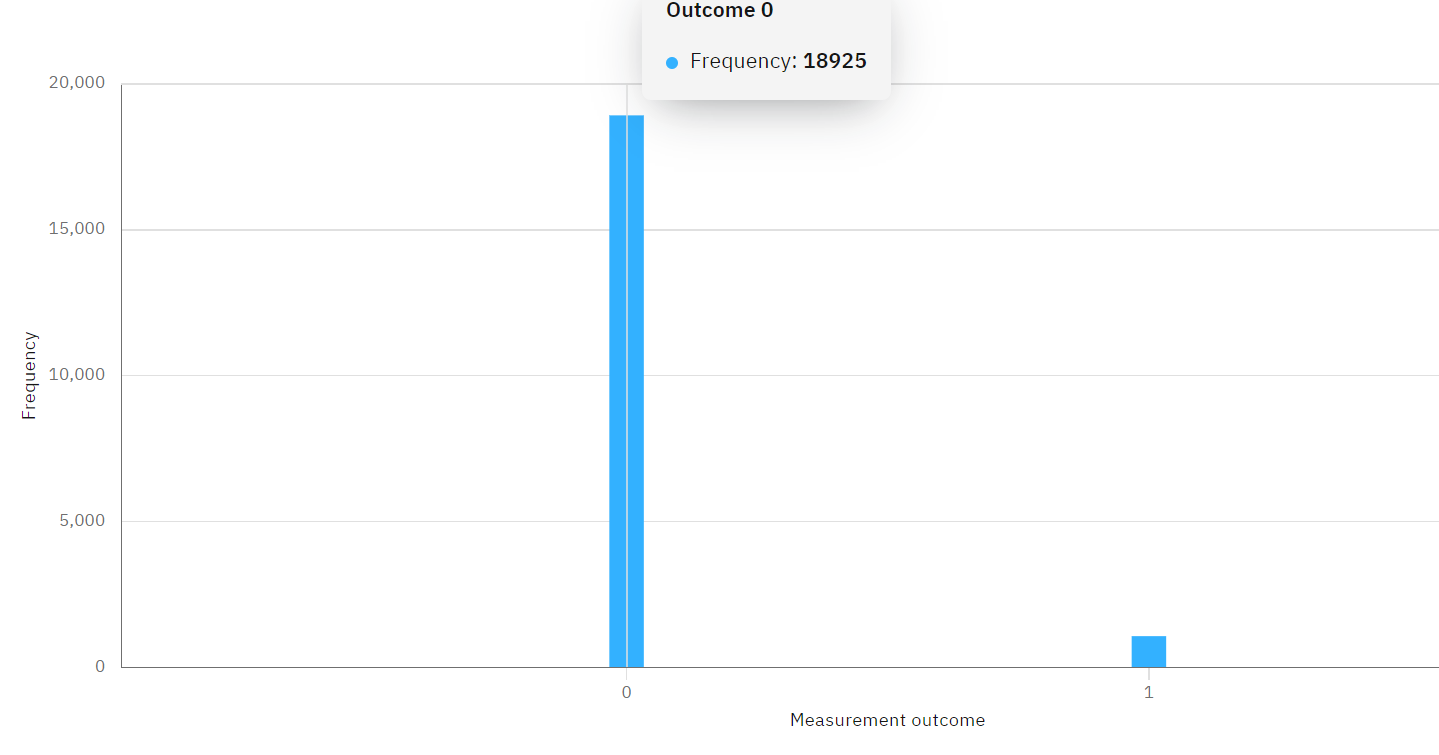
\includegraphics[width=\columnwidth]{qpe_1qubit_Messung.PNG}
  \centering
  \end{figure}
  

Die Präzision der Quantum-Phase-Estimation lässt sich durch die Verwendung mehrerer Qubits erhöhen.
Diese zusätzlichen Qubits dienen als weitere Kontrollqubits.
Die Anzahl der Qubits, die für den Eigenvektor benötigt werden, 
bleibt unverändert und entspricht der Bitanzahl, 
die ausreicht, um den Wert des Eigenvektors zu definieren.
Jedes einzelne Kontrollqubit kontrolliert ein \(U^{2^x}\)-Gatter.
Bei \(n\) Kontrollqubits kontrolliert das least-significant-bit ein \(U^{2^0}\)-Gatter,
das darauffolgende ein \(U^{2^1}\)-Gatter und so weiter,
bis das letzte Kontrollqubit ein \(U^{2^{n-1}}\)-Gatter kontrolliert.
\(U^{2^x}\) kann entweder durch \(2^x\) viele \(U\)-Gatter oder durch ein einzelnes Gatter implementiert werden, 
das den Eigenwert \(\lambda\) mit \(2^x\) multipliziert anwendet.
Anschließend wird die inverse Quanten-Fourier-Transformation auf alle Kontrollqubits angewendet.
Durch die Messung lässt sich dann der Wert für \(\varphi\) ermitteln.
Der Aufbau der Schaltung ist als Skizze in Abbildung~\ref{fig:qpe_n_qubit} abgebildet.

\begin{figure}[H]
  \centering
  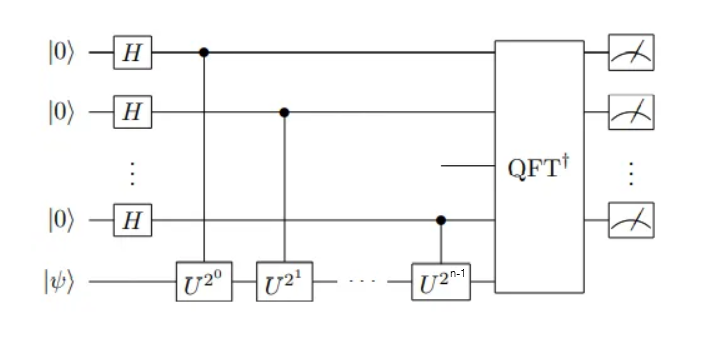
\includegraphics[scale = 0.8]{qpe_n_qubit.PNG}
  \caption{N Qubit QPE}
  \label{fig:qpe_n_qubit}
\end{figure}

Wird die Quanten-Fourier-Transformation wie in Abbildung~\ref{fig:qpe_n_qubit} realisiert,
kann man den Zustand der Kontrollqubits vor der inversen Quanten-Fourier-Transformation wie folgt beschreiben:
\[\frac{1}{\sqrt{N}}\Bigg[
  CU^{2^0}\Big(\ket{0} + \ket{1}\Big) \tensor
  CU^{2^1}\Big(\ket{0} + \ket{1}\Big) \tensor 
  ... \tensor
  CU^{2^{n-1}}\Big(\ket{0} + \ket{1}\Big) 
  \Bigg]\]
Mit \(U^{2^x}\ket{x}_n=e^{2\pi i 2^x\varphi}\ket{x}_n\) wird der Eigenwert \(e^{2\pi i \varphi}\) wegen des Phase-Kickbacks
über die \(CU\)-Gatter auf die Kontrollqubits übertragen:
\[\frac{1}{\sqrt{N}}\Bigg[
  \Big(\ket{0} + e^{2\pi i 2^0 \varphi}\ket{1}\Big) \tensor
  \Big(\ket{0} + e^{2\pi i 2^1 \varphi}\ket{1}\Big) \tensor 
  ... \tensor
  \Big(\ket{0} + e^{2\pi i 2^{n-1} \varphi}\ket{1}\Big) 
  \Bigg]\]
Schreibt man \(\varphi\) als Binärbruch:
\[\varphi = \frac{\varphi_n}{2^1} + \frac{\varphi_{n-1}}{2^2} + ... + \frac{\varphi_1}{2^n}\]
Kann die Formel in einer ähnlichen Form wie die Quanten-Fourier-Transformation umgeformt werden:
\begin{align*}
\frac{1}{\sqrt{N}}\Bigg[
  \Big(\ket{0} + e^{2\pi i (\frac{\varphi_n}{2})} 
  ...  
  e^{2\pi i (\frac{\varphi_2}{2^{n-1}})}e^{2\pi i (\frac{\varphi_1}{2^{n}})}\ket{1}\Big) 
  \tensor ... 
  &\tensor
  \Big(\ket{0} +  e^{2\pi i (\frac{\varphi_2}{2})}e^{2\pi i (\frac{\varphi_1}{4})}\ket{1}\Big)\\ 
  &\tensor 
  \Big(\ket{0} + e^{2\pi i (\frac{\varphi_1}{2})}\ket{1}\Big) 
  \Bigg]
\end{align*}
Die Formel besitzt die gespiegelte Struktur wie die Quanten-Fourier-Transformation ohne Swap-Gatter:
\begin{align*}
  QFT_{N}\ket{x}_{n} = 
  \frac{1}{\sqrt{N}}
  \Bigg[
    \Big(\ket{0} + { e^{2 \pi i (\frac{x_1}{2})}}\ket{1}\Big) 
    &\tensor
    \Big( \ket{0} + { e^{2 \pi i (\frac{x_2}{2})(\frac{x_1}{4})}}\ket{1}\Big)\\
    &\vdotswithin{\tensor}\\
    &\tensor
    \Big(\ket{0} + e^{2\pi i (\frac{x_n}{2})} ... e^{2\pi i (\frac{x_2}{2^{n-1}})}e^{2\pi i (\frac{x_1}{2^{n}})}\ket{1}\Big)
  \Bigg]
\end{align*}
Durch die Verwendung der Swap-Gatter kann die Reihenfolge der Quanten-Fourier-Transformation gespiegelt werden, 
anschließend sind beide Formeln strukturell identisch.

Wie im Abschnitt zur Quanten-Fourier-Transformation erklärt,
transformiert die Quanten-Fourier-Transformation den Zustand der Eingangsqubits \(\ket{x}_n\) in die Phasen der Ausgangsqubits.
Im Gegensatz dazu kehrt die inverse Quanten-Fourier-Transformation diesen Vorgang um, 
indem die Phaseninformationen der Eingangsqubits in Zustände der Standardbasis transformiert werden.

Die Anwendung der inversen Quanten-Fourier-Transformation, inklusive Swap-Gatter, bewirkt also:
\begin{align*}
iQFT\Bigg(
\frac{1}{\sqrt{N}}
\Bigg[
  \Big(\ket{0} + e^{2\pi i (\frac{\varphi_n}{2})} ...& e^{2\pi i (\frac{\varphi_2}{2^{n-1}})}e^{2\pi i (\frac{\varphi_1}{2^{n}})}\ket{1}\Big) \\
  &\vdotswithin{\tensor}\\
  &\tensor
  \Big(\ket{0} +  e^{2\pi i (\frac{\varphi_2}{2})}e^{2\pi i (\frac{\varphi_1}{4})}\ket{1}\Big) \tensor 
  \Big(\ket{0} + e^{2\pi i (\frac{\varphi_1}{2})}\ket{1}\Big) 
  	\Bigg]
\Bigg)
\end{align*}
\[ = \ket{\varphi_1 \varphi_{2}...\varphi_n}_n = \ket{2^n\varphi}_n\]
Schließlich kann \(\varphi\) mit einer Division durch \(2^n\) bestimmt werden.

Als Beispiel wird die Quantum-Phase-Estimation für
\(U\ket{1}_1=e^{2\pi i \frac{3}{8}}\ket{1}_1\), 
also mit \(\varphi = \frac{3}{8}\) betrachtet.
Im Quantenschaltkreis aus Abbildung~\ref{fig:3_qubit_qpe} 
werden die kontrollierten \(U^{2^x}\)-Gatter als Phase-Gatter mit steigendem \(x\) in \(P(2^x 2\pi \frac{3}{8})\) realisiert.
\begin{figure}[H]
  \centering
  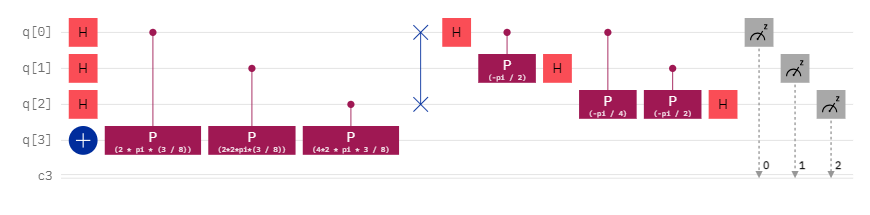
\includegraphics[width=\columnwidth]{3_qubit_qpe.png}
  \caption{3-Kontroll-Qubit QPE}
  \label{fig:3_qubit_qpe}
\end{figure}
Die Messung in Abbildung~\ref{fig:3_qubit_qpe_measurement} ergibt konsistent bei allen Durchläufen den Zustand \(\ket{3}_3\).
Da \(\ket{3}_3 = \ket{2^3\varphi}_3\) entspricht, 
lässt sich durch eine Division \(\varphi = \frac{3}{8}\) ermitteln.
Es ist zu beachten, 
dass die Reihenfolge der Wertigkeit der Qubits gleich bleibt.
Normalerweise tauschen die inverse wie auch die normale Quanten-Fourier-Transformation die Wertigkeiten.
Dieser Effekt wird jedoch durch Swap-Gatter korrigiert.
\begin{figure}[H]
  \centering
  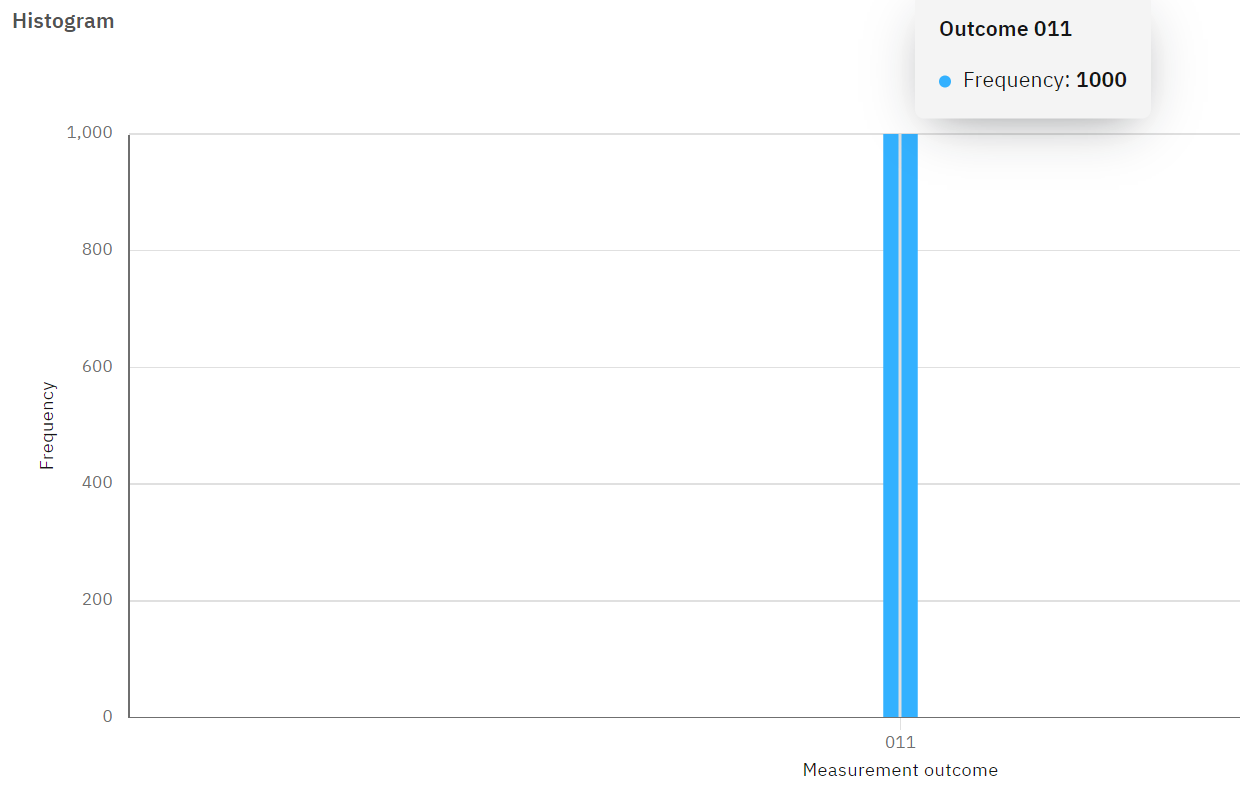
\includegraphics[width=\columnwidth]{3_qubit_qpe_measurement.PNG}
  \caption{3-C-Qubit QPE Messergebnis}
  \label{fig:3_qubit_qpe_measurement}
\end{figure}

Im vorherigen Beispiel liefern die Messungen aller Durchläufe den gleichen Zustand, 
mit dem \(\varphi\) eindeutig bestimmbar ist.
Diese Eindeutigkeit tritt auf, 
wenn die verwendete Anzahl an Kontroll-Qubits ausreicht, 
um \(\varphi\) eindeutig zu repräsentieren.
Im obigen Beispiel kann \(\varphi\) eindeutig mit den drei verwendeten Kontrollqubits dargestellt werden:
\[{\frac{3}{8} =0 \cdot 2^{-1} + 1\cdot2^{-2} + 1\cdot2^{-3}}\]
Verwendet man nicht ausreichend Kontroll-Qubits, 
kann \(\varphi\) nicht eindeutig repräsentiert werden.
Als Konsequenz wird die Messung ungenau.
Mit hoher Wahrscheinlichkeit kollabieren die Qubits bei einer Messung 
in die darstellbaren Zustände, 
die den genauen Wert am besten approximieren.
Dabei liegt die Wahrscheinlichkeit, dass die Messung in einen der beiden angrenzenden Zustände kollabiert, 
bei mindestens \(\frac{8}{\pi^2}\)~\cite[119]{kaye2007introduction}.

In Abbildung~\ref*{fig:3_qubit_qpe_measurment_uncertain} sind die Messergebnisse einer Quantum-Phase-Estimation abgebildet, 
die die Phase \(\varphi = \frac{5}{16}\) bestimmen soll.
Da \(\frac{5}{16}\) nicht mit 3 Qubits darstellbar ist, 
gibt es kein eindeutiges Messergebnis.
Anhand der Messergebnisse ist aber erkennbar, 
dass die Messungen mit einer Wahrscheinlichkeit größer als \(\frac{8}{\pi^2}\) in
einen der beiden angrenzenden Zustände kollabiert.
Diese entsprechen \({\frac{2}{8} = \frac{4}{16}}\) und \({\frac{3}{8} = \frac{6}{16}}\), 
also genau den Werten, die \(\frac{5}{16}\) am nächsten sind.

\begin{figure}[H]
  \centering
  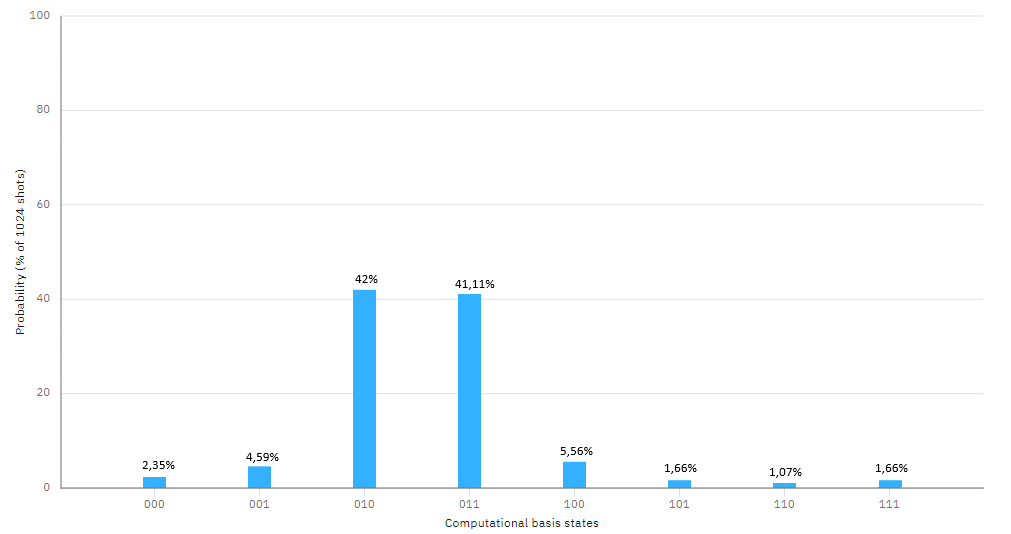
\includegraphics[width=\columnwidth]{3_qubit_qpe_measurment_uncertain.PNG}
  \caption{QPE unpräzises Messergebnis}
  \label{fig:3_qubit_qpe_measurment_uncertain}
\end{figure}












 






 












\section{Shor-Algorithmus}
Im folgenden Kapitel wird der Shor-Algorithmus zum Faktorisieren von Zahlen beschrieben.
Der Inhalt bezieht sich auf den Zweck, die Funktionsweise und den Aufbau des Algorithmus.
Der Aufbau beinhaltet nicht die konkrete Implementierung der Bestandteile des Algorithmus.
Stattdessen werden die Details bezüglich der Implementierung im nächsten Kapitel behandelt.

\subsection{Zweck}
Der Shor-Algorithmus wurde mit dem spezifischen Ziel entwickelt, 
große zusammengesetzte Zahlen effizient auf Quantencomputern in ihre Primfaktoren zu faktorisieren. 
Im Gegensatz zu klassischen Faktorisierungsverfahren, die exponentielle Zeit erfordern~\cite{katz2023}, 
ermöglicht Shor's Ansatz die Faktorisierung in polynomialer Zeit, 
in Bezug auf die Anzahl an Bits der zu faktorisierenden Zahl~\cite{Shor_1997}. 
Dies stellt eine signifikante Beschleunigung gegenüber den besten bekannten klassischen Faktorisierungsverfahren dar.
Der Shor-Algorithmus bekräftigt die These, das Quantencomputer
bestimmte Probleme wesentlich schneller lösen können als ihre klassischen Gegenstücke.

\subsection{Funktionsweise} \label{Funktionsweise}
Der Shor-Algorithmus verwendet zwei Teilberechnungen, die zusammen die Faktorisierung berechnen.
Die erste Teilberechnung erfolgt mittels eines Quantenalgorithmus. 
Der zweite Teil basiert auf einem klassischen Algorithmus.
Im quantenmechanischen Teil des Shor-Algorithmus geht es um die Bestimmung der Ordnung in der multiplikativen Gruppe modulo \(N\).
Hierbei ist anzumerken, dass der Quantenalgorithmus nicht direkt die Primfaktoren der zu faktorisierenden Zahl berechnet.
Stattdessen wird die Eigenschaft ausgenutzt, 
dass das Problem der Faktorisierung äquivalent zu dem Problem der Ordnungsbestimmung ist~\cite{nielsen_chuang_2010}.
Daher impliziert eine effiziente Lösung für die Berechnung der Ordnung eine ebenso effiziente Methode zur Faktorisierung.
Der nachfolgende klassische Algorithmus verwendet die ermittelte Ordnung, 
um die Primfaktoren abzuleiten. 
Beide Teilberechnungen, sowohl die quantenmechanische als auch die klassische, 
führen ihre Berechnungen in polynomialer Zeit durch. 
Daher liegt die gesamte Laufzeit des Shor-Algorithmus ebenfalls in einer polynomialen Größenordnung.

\subsection{Ordnungsbestimmung} \label{Shor:Ordnungsbestimmung}
Zu bestimmen sind die Primfaktoren der Zahl \(N\).
Zuerst wird ein \(a\) mit \(0 < a < N\) gewählt.
Falls der ungewöhnlichen Fall eintritt, dass \(a\) nicht teilerfremd zu \(N\) ist, entspricht \(a\) einem der Primfaktoren.
Anschließend wird die Ordnung beziehungsweise Periode \(p\) der Funktion \({f(x) = a^x \mod N}\) mit einem Quantenalgorithmus bestimmt:

Die Periode \(p\) beschreibt das kleinste ganzzahlige Element mit \({p > 0}\), für das gilt: \({f(p) = 1 \mod N}\).
\[
\begin{tabular}{l|llllll}
    x     &     0     &     1       &     2      &      3   &  4 &  5  \\ \hline
    \(7^x \mod 15\)    &      1     &        7     &       4     &     13     &  1 &  7 
\end{tabular} \longmapsto p = 4
\]

Im Wesentlichen handelt es sich bei der quantenmechanischen Berechnung des Shor-Algorithmus um die Quanten-Phase-Estimation.
Die Architektur dieser spezifischen Quanten-Phase-Estimation korrespondiert weitgehend mit der in Abschnitt~\ref{Quanten-Phase-Estimation} vorgestellten Struktur.
Hierbei ersetzen speziell für die gegebene Anwendung definierte \(U\)-Gatter die allgemeinen.

Für den konkreten Kontext der Periodenberechnung, realisieren die \(U\)-Gatter die Transformation:
\[U\ket{y} = \ket{ay \mod N}\] 
Die Ausführung der Quanten-Phase-Estimation erfordert die Erzeugung eines Eigenvektors der Transformation \(U\).
Da die Quanten-Phase-Estimation \(\varphi\) aus dem Eigenwert extrahiert, 
darf der Eigenvektor nicht den trivialen Eigenwert 1 besitzen.
Stattdessen ist es notwendig, dass die Periode der Transformation im Eigenwert enthalten ist.

Wie in~\autocite[227]{nielsen_chuang_2010} gezeigt wird, gibt es zu \(U\) Eigenvektoren \(\ket{u_s}\), 
mit \(0 \leq s \leq p-1\): 
\[\ket{u_s} \equiv
\frac{1}{\sqrt{p}}
\sum_{k=0}^{p-1} e^{\frac{-2 \pi i s k}{p}\ket{a^k \mod N}} %ich soll die Formel mit der Summe sein
\]
Für \(a=7\) bei \(N=15\) entspricht \(r=4\).
Ein Eigenvektor zu \(s=1\) lautet dann:
\[
    \ket{u_1}_4 =
    \frac{1}{\sqrt{4}}(
        \ket{1}_4 + 
        e^{-\frac{2 \pi i}{4}}\ket{7}_4 + 
        e^{-\frac{4 \pi i}{4}}\ket{4}_4+ 
        e^{-\frac{6 \pi i}{4}}\ket{13}_4
    )
    \]
\[
    U\ket{u_1}_4 =
    \frac{1}{\sqrt{4}}(
        \ket{7}_4 + 
        e^{-\frac{2 \pi i}{4}}\ket{4}_4 + 
        e^{-\frac{4 \pi i}{4}}\ket{13}_4+ 
        e^{-\frac{6 \pi i}{4}}\ket{1}_4
    )
    \]
\[
    U\ket{u_1}_4 =
    e^{\frac{2 \pi i}{4}}
    \cdot
    \frac{1}{\sqrt{4}}(
        e^{-\frac{2 \pi i}{4}}\ket{7}_4 + 
        e^{-\frac{4 \pi i}{4}}\ket{4}_4 + 
        e^{-\frac{6 \pi i}{4}}\ket{13}_4+ 
        e^{-\frac{8 \pi i}{4}}\ket{1}_4
    )
    \]
\[
    U\ket{u_1}_4 =
    e^{\frac{2 \pi i}{4}}
    \cdot
    \frac{1}{\sqrt{4}}(
        e^{-\frac{8 \pi i}{4}}\ket{1}_4
        e^{-\frac{2 \pi i}{4}}\ket{7}_4 + 
        e^{-\frac{4 \pi i}{4}}\ket{4}_4 + 
        e^{-\frac{6 \pi i}{4}}\ket{13}_4 )
    =
    e^{\frac{2 \pi i}{4}} \cdot
    \ket{u_1}_4
    \]
Das kann verallgemeinert werden:
\[U\ket{u_s} = e^{\frac{2 \pi i s}{p}}\ket{u_s}\]

Wie man in der Definition von \(\ket{u_s}\) %ref zu Formel mit der Summe
sieht, 
benötigt die Initialisierung eines Eigenvektors \(\ket{u_s}\) mit einem konkreten \(s\) die Periode \(p\).
Man kann diese Problematik jedoch umgehen indem man anstelle eines einzelnen Eigenvektors \(\ket{u_s}\)
eine Superposition verwendet, die alle \(\ket{u_s}\) umfasst.
Die Superposition entspricht~\autocite[227]{nielsen_chuang_2010}:
\[\frac{1}{\sqrt{p}} \sum_{s=0}^{r-1}\ket{u_s} = \ket{1}\] 
Also wird das Qubit, welches das Least-Significant-Bit des für den Eigenvektor bestimmten Qubit-Registers repräsentiert, 
mit \(\ket{1}\) initialisiert.

Die Superposition der Eigenvektoren hat zur Folge, 
dass nach der inversen Quanten-Fourier-Transformation, also am Ende der Quanten-Phase-Estimation,
ebenfalls eine Superposition mit dem \(\varphi_s\) der Eigenwerte \(\lambda_{u_s}\) aller möglichen Eigenvektoren \(\ket{u_s}\) existiert.
Sei \(k\) die Anzahl an Kontroll-Qubits dann:
\[
    \frac{1}{\sqrt{p}} \sum_{s=0}^{p-1}\ket{2^k \cdot \frac{s}{p}}_k   = 
    \frac{1}{\sqrt{p}} (\ket{0}_k  + \ket{2^k \cdot \frac{1}{p}}_k + \ket{2^k \cdot \frac{2}{p}}_k  ... + \ket{2^k \cdot \frac{p-1}{p}}_k )
    \]


Bei einer Messung wird also zufällig eines der insgesamt \(p\) vielen \(\varphi_s \approx \frac{s}{p}\) gemessen.

Die Genauigkeit des Algorithmus, ausgedrückt durch den Parameter \(k\),
ist direkt abhängig von der Anzahl der verwendeten \(U^{2^x}\)-Gatter
und der damit assoziierten Kontroll-Qubits im Quantenschaltkreis.
Die Genauigkeit des Messergebnisses gegenüber dem \(\varphi_s\) hängt von \(k\) ab.

Wenn genügend Kontroll-Qubits verwendet werden, 
wird bei einer Messung ein Zustand gemessen, 
in welchem \(\frac{s}{p}\) enthalten ist.

Falls nicht ausreichend Kontroll-Qubits vorhanden sind 
und der Wert von \(\varphi_s\) somit nicht ausreichend umfasst werden kann,
wird die Messung mit hoher Wahrscheinlichkeit 
in einen der möglichen Zustand kollabieren, 
der dem genauen Ergebnis am nächsten ist. 
Dadurch bilden sich ein Peak rund um den korrekten Wert, 
welcher Vergleichbar ist mit Abbildung~\ref{fig:3_qubit_qpe_measurment_uncertain}.
Genau wie in Abbildung~\ref{fig:3_qubit_qpe_measurment_uncertain}, haben die Werte nah dem genauen Wert
eine höhere Chance gemessen zu werden. 
Da aber eine Messung von probabilistischer Natur ist, 
kann eine Messung auch zu einem Ergebnis führen, 
welches entfernt vom genauen Ergebnis liegt.

Anders als in Abbildung~\ref{fig:3_qubit_qpe_measurment_uncertain} gibt es bei der Periodenbestimmung insgesamt \(p\) Peaks.
Das liegt daran, dass es insgesamt \(p\) viele Zustände in der Superposition des Endzustandes gibt.

Anhand des Messergebnisses erfolgt die Primfaktorzerlegung in einer Nachberechnung.

\subsection{Klassische Nachberechnung} \label{Funktionsweise:klassisch}
Die Nachberechnung benötigt keine Quantenbrechnung und 
wird somit mit einem klassischen Algorithmus durchgeführt.

Ein einzelner Zustand der finalen Superposition, 
entspricht einem genauen Ergebnis und besitzt die Form \(\ket{2^k \cdot \frac{s}{p}}_k\) für \(0 \leq s < p\).
Mit einer Division durch \(2^k\) kann \(\frac{s}{p}\) extrahiert werden.
Zum Beispiel ist die finale Superposition für \(a = 7;~N=15\) mit \(p=4\) bei einer Genauigkeit \(k=4\):
\[\frac{1}{\sqrt{4}}(\ket{0}_4 +\ket{2^4 \cdot \frac{1}{4}}_4 + \ket{2^4 \cdot \frac{2}{4}}_4+\ket{2^4 \cdot \frac{3}{4}}_4) =
 \frac{1}{\sqrt{4}}(\ket{0}_4 +\ket{4}_4 + \ket{8}_4+\ket{12}_4) \]
Mit Ausnahme der Zustände \(\ket{0}_4\) und \(\ket{8}_4\), 
gewähren die beiden anderen Zustände nach einer Division mit \(2^4\) eine Kommazahl, 
die als Bruch die gesuchte Periode \(p=4\) als Nenner enthält.

Im vorherigen Beispiel handelt es sich bei der Periode um eine 2er Potenz, 
weswegen die Messergebnisse eindeutig sind.
Jedoch ist dies ein ideales Szenario welches bei immer größeren \(N\) seltener auftretet. 
Das nächste Beispiel beachtet \(a=11;~N=21\) mit der Periode \(p=6\) bei einer Genauigkeit \(k=4\):
\[\frac{1}{\sqrt{6}}(\ket{0}_4 +\ket{2^4 \cdot \frac{1}{6}}_4 + \ket{2^4 \cdot \frac{2}{6}}_4+
\ket{2^4 \cdot \frac{3}{6}}_4)+\ket{2^4 \cdot \frac{4}{6}}_4 + \ket{2^4 \cdot \frac{5}{6}}_4 \]
\[= \frac{1}{\sqrt{6}}(\ket{0}_4 +\ket{2,\overline{6}}_4 + \ket{5,\overline{3}}_4+
\ket{8}_4+\ket{10,\overline{6}}_4 + \ket{13,\overline{3}}_4) \]
Die Kontroll-Qubits, welche gemessen werden, 
können keine Kommazahlen darstellen.
Als Folge davon, bildet sich um die benachbarten Zustände eine Wahrscheinlichkeitsverteilung, 
die bei dem ganzzahligen Zustände, der am nächst liegt, ihren Hochpunkt hat,
vergleichbar mit~\ref{fig:3_qubit_qpe_measurment_uncertain}.
Im konkreten Beispiel wird für \(\ket{2,\overline{6}}_4\) der Zustand \(\ket{3}_4\) 
mit der höchsten Wahrscheinlichkeit gemessen.
Eine Extraktion der Periode aus \(\ket{3}_4\)  mit \(\frac{3}{2^4}\) liefert als Ergebnis die Kommazahl \(0,1875\).
Mit dem Kettenbruch-Algorithmus wird zu der Kommazahl der nächstgelegene Bruch gefunden, 
im konkreten Fall die \(\frac{3}{16}\).
Der Bruch \(\frac{3}{16}\) enthält im Nenner nicht die gesuchte Periode \(p=6\). 
Das Gleiche gilt auch für andere Zustände, 
die mit hoher Wahrscheinlichkeit gemessen werden können, wie 
\(\ket{5}_4,~\ket{8}_4,~\ket{11}_4\) und \(\ket{13}_4\).

Das Versagen der vorausgegangenen Berechnung ist auf eine unzureichende Genauigkeit zurückzuführen. 
In der vorangegangenen Darstellung werden \(k=4\) Kontroll-Qubits eingesetzt, 
welche für die gesuchte Periode einen zu kleinen Wertebereich bilden.

Wiederholt man das ganz, mit \(k=7\), erhält man folgende Superposition:
\[\frac{1}{\sqrt{6}}(\ket{0}_7 +\ket{21,\overline{3}}_7 + \ket{42,\overline{6}}_7+
\ket{64}_7+\ket{85,\overline{3}}_7 + \ket{106,\overline{6}}_7) \]
Es ist ersichtlich, dass die genauen Zustände weiterhin über Nachkommastellen verfügen.
Weswegen mit einer geringeren Wahrscheinlichkeit auch andere Werte gemessen werden können.
Bei einer Messung ist statt des Zustands \(\ket{21,\overline{3}}_7\) der Zustand \(\ket{21}_7\) das wahrscheinlichste Ergebnis.
Für \(\frac{21}{2^{7}}\) erhält man eine Kommazahl, deren genauer Bruch \(\frac{21}{128}\) entspricht.
Bekanntlich entspricht die Periode jedoch einer Zahl \(p\) die kleiner ist als \(N\).
Wendet man auf \(\frac{21}{128}\) den Kettenbruch-Algorithmus an und limitiert den Nenner auf \(N\), 
wird der nächstgelegene Bruch gefunden, welcher ein Nenner besitzt, der kleiner ist als \(N\).
Im konkreten Beispiel folgt für \(\frac{21}{128}\) der Bruch \(\frac{1}{6}\), 
welcher die Periode im Nenner offenbart.
Bei einer Messung kann auch der benachbarte ganzzahlige Zustand \(\ket{22}_7\) gemessen werden, 
allerdings mit einer geringeren Wahrscheinlichkeit im Vergleich zu \(\ket{21}_7\).
Der Zustand \(\ket{22}_7\) ermöglicht nicht die Extraktion der Phase, 
da \(\frac{22}{128}\) mit dem Kettenbruch-Algorithmus auf einen für \(N\) limitierten Nenner
zu \(\frac{3}{17}\) wird.

Bedeutet mit einer hinreichenden Genauigkeit, kann die Periode nur aus dem Zustand extrahiert werden, 
welcher den Wert des genauen Zustandes am besten approximiert.

Mit zusätzlichen Kontroll-Qubits wird das Messergebnis Fehlertolerant.
Wiederholt man das Beispiel erneut, diesmal jedoch mit \(k=10\), 
ist der zweite Zustand in der finalen Superposition: 
\(\ket{2^{10} \cdot \frac{1}{6}}_{10} =\ket{170,\overline{6}}_{10}\).
Im Gegensatz zu vorher liefert jetzt nicht nur das am besten approximierte Ergebnis, 
in dem Fall die \(\ket{170}_{10}\), mit dem Kettenbruch-Algorithmus die Periode, 
sondern auch alle benachbarten Zustände von \(\ket{167}_{10}\) bis \(\ket{175}_{10}\).

Durch den Einsatz von zusätzlichen Kontroll-Qubits erhöht sich der Wertebereich. 
Aufgrund des größeren Wertebereiches existieren mehr mögliche Zustände, 
die bei einer Messung vorkommen könnten und ebenfalls auch mehr Zustände, 
die die Extraktion der korrekten Periode ermöglichen. 
Dabei ist die Wahrscheinlichkeitsverteilung der ausschlaggebende Faktor. 
Diese verändert sich mit einer wachsenden Anzahl an Kontroll-Qubits zugunsten der Zustände, 
welche die korrekte Periode offenbaren.
Die Abbildungen~\ref{fig:Messung7k} und~\ref{fig:Messung10k} 
heben den Effekt zusätzlicher Kontroll-Qubits auf die Wahrscheinlichkeitsverteilung der Messungen hervor.
Die grünen Säulen im Diagram zeigen die Messergebnisse, welche die Extraktion der Periode erlauben.

\begin{figure} [H]
    \caption{Messergebnisse für a=11, N=21, k=7 bei 1024 Messungen}
    \label{fig:Messung7k}
    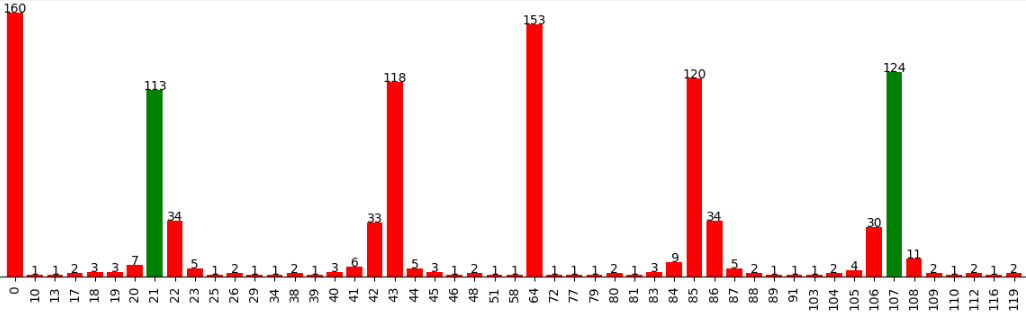
\includegraphics[scale = 0.55]{wahrscheinlichkeit_k7.PNG}
    \centering
    \end{figure}
\begin{figure} [H]
    \caption{Messergebnisse für a=11, N=21, k=10 bei 1024 Messungen}
    \label{fig:Messung10k}
    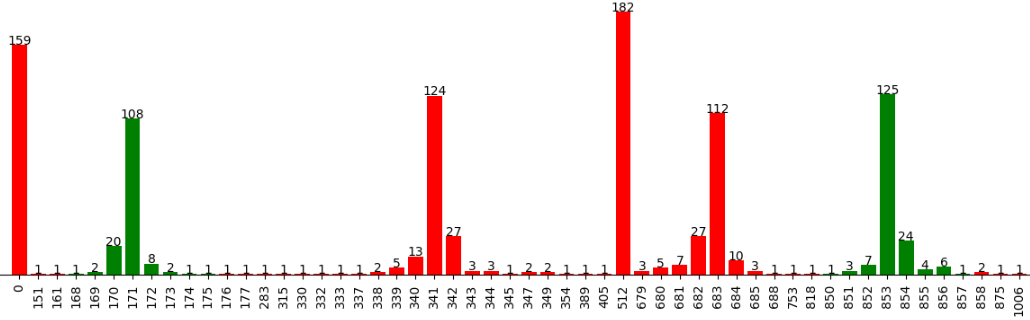
\includegraphics[scale = 0.55]{wahrscheinlichkeit_k10.PNG}
    \centering
    \end{figure}

Für eine bekannte Periode, 
kann man zeigen, 
dass die Verwendung von \(k > 2\text{ld}(p)\) eine ausreichende Genauigkeit liefert,
so dass ein Messergebnis unter Verwendung des Kettenbruch-Algorithmus zu einem Näherungsbruch \(\frac{s}{p}\) von \(\varphi_s\) konvergiert~\cite{Shor_1997}.
Im Normalfall kann für eine Elementes \(a\) für den Modulus \(N\) vorab nicht gesagt werden, 
wie viele Kontroll-Qubits man exakt braucht, 
da dies von der unbekannten Periode \(p\) abhängt.
Stattdessen, verwendet man einen Wert der auf alle Fälle größer als \(2\text{ld}(p)\) ist, 
wie zum Beispiel \(2\text{ld}(N)\)~\cite{Shor_1997}\cite{mosca1999hidden}. 

Wie man in Abbildungen~\ref{fig:Messung10k} sieht, 
gibt es auch bei der Verwendung von \(2\text{ld}(N)\) Kontroll-Qubits drei Szenarien, 
bei denen eine Zustand mit einer ungültigen Periode gemessen werden kann.

Im Falle des ersten Szenarios, 
entspricht mindestens einer der Zustände der finalen Superposition einer Kommazahl.
Dadurch kann es zu Messungen von falschen Werten kommen.
Anhand dieses Ergebnisses führt der Kettenbruch-Algorithmus nicht zu \(\frac{s}{p}\), 
weswegen eine neue Messung benötigt wird.

Das zweite Szenario ähnelt dem ersten und tritt ebenfalls auf, 
sobald mindestens einer der Zustände der finalen Superposition eine Kommazahl ist. 
Im Unterschied zum ersten Szenario liegt dieses Messergebnis jedoch nah bei einem Peak, 
also in der Nähe eines Messergebnisses, aus dem die Periode extrahiert werden kann. 
Indem man die Nachbarzustände des Messergebnisses testet, kann man gegebenenfalls einen Zustand finden, 
der die Extraktion der Periode ermöglicht.

Das zweite Szenario tritt beispielsweise für das Messergebnis \(\ket{176}_{10}\) in Abbildung~\ref{fig:Messung10k} auf.
Die Anwendung des Kettenbruch-Algorithmus auf \(\frac{176}{2^{10}}\) 
liefert nicht die korrekte Periode, stattdessen ergibt sich der Bruch \(\frac{3}{17}\). 
Anstatt eine neue Messung durchzuführen,
ist es in diesem Fall zielführend, 
die ganzzahligen Nachbarn des Messergebnisses zu überprüfen.
Im konkreten Beispiel ermöglicht bereits die geringfügige Anpassung des Messergebnisses durch Subtraktion von 1, 
also zu \(\ket{175}_{10}\), 
die erfolgreiche Extraktion der Periode.

Die Erhöhung der Genauigkeit \(k\) auf Werte über \(2\text{ld}(N)\) hinaus hat den Effekt, 
dass die Wahrscheinlichkeit für das Eintreten des ersten oder zweiten Falls abnimmt.
Dadurch verbessern sich gleichzeitig die Wahrscheinlichkeit, direkt ein korrektes Ergebnis zu messen.
Allerdings führt dies zu einem komplexeren Quantenschaltkreis und 
somit erhöhen sich die Kosten an zusätzlichen Ressourcen~\autocite[231]{nielsen_chuang_2010}.

Der dritte und letzte Fall kann immer auftreten.
In diesem Szenario wird ein \(\frac{s'}{p'}\) gemessen, 
welches entsteht, wenn \(s\) und \(p\) einen gemeinsamen Teiler haben und 
deswegen von \(\frac{s}{p}\) auf \(\frac{s'}{p'}\) gekürzt wurden.
In diesem Fall kann ein vielfaches von \(p'\), also \(2p'\),\(3p'\),.. zum richtigen \(p\) führen.
Des Weiteren besteht die Möglichkeit, 
dass bei einer zweiten Messung erneut ein gekürztes \(\frac{s}{p}\) als \(\frac{s''}{p''}\) gefunden wird.
Wenn \(s'\) und \(s''\) keine Faktoren teilen,
kann aus dem kleinsten gemeinsamen Vielfachen von \(p'\) und \(p''\) das \(p\) berechnet werden~\cite{Shor_1997}.

In Abbildung~\ref{fig:Messung10k} sind die beiden Peaks um die Zustände \(\ket{341}_{10}\) und \(\ket{683}_{10}\) rot gefärbt, 
was auf den dritten Fall zurückzuführen ist.
Sowohl \(\ket{341}_{10}\) als auch \(\ket{683}_{10}\) und ihre benachbarten Zustände 
enthalten ursprünglich im Nenner die korrekte Periode, wurden jedoch gekürzt.
Die Brüche wurden auf \(\frac{1}{3}\), beziehungsweise \(\frac{2}{3}\), gekürzt. 
Eine Überprüfung der nächsten Vielfachen, in diesem Fall \(2 \cdot 3 = 6 \), führt zur korrekten Periode.

Man kann zeigen, dass man mit mindestens einer Wahrscheinlichkeit von \(\frac{1}{2\text{ld}(N)}\), 
bei einer Messung ein \(s\) bekommt, welches eine Primzahl ist und somit zu \(p\) teilerfremde ist.
Das bedeutet, dass bei insgesamt \(2\text{ld}(N)\) Messungen, die Wahrscheinlichkeit sehr hoch ist, mindestens einmal ein \(\frac{s}{p}\)
zu messen, bei dem \(s\) und \(p\) nicht gekürzt sind~\autocite[231]{nielsen_chuang_2010}.

Ob die korrekte Periode gefunden wurde, kann mit \(a^p = 1 \mod N\) geprüft werden.

Sobald die korrekte Periode \(p\) gefunden wurde, 
können die Primfaktoren von \(N\) mit dem größten gemeinsamen Teiler(gcd) berechnet werden:
\[gcd(a^{\frac{p}{2}}-1, N), gcd(a^{\frac{p}{2}}+1, N)\]
Dies schlägt nur fehl falls \(p\) ungerade ist
oder falls \(a^{\frac{p}{2}} = -1 \mod N\) erfüllt~\cite{Shor_1997}.
Die Wahrscheinlichkeit dass einer der beiden genannten Fälle eintritt beträgt \(1-\frac{1}{2^f}\), 
wobei \(f\) die Anzahl an unterschiedlicher Primfaktoren von \(N\) angibt~\cite{Shor_1997}.
In einem solchen Fall, wiederholt man die Periodenberechnung mit einem anderen \(a\).


\section{Implementierung} \label{sec:Implementierung}

\subsection{Quantenalgorithmus}
Wie im Kapitel~\ref{Funktionsweise} zur Funktionsweise erklärt,
wird für die Periodenbestimmung die Quantum-Phase-Estimation genutzt.

Um den Quantum-Phase-Estimation Algorithmus für die Periodenberechnung zu nutzen,
benötigt man ein \(U\)-Gatter, 
welches die modulare Multiplikation, 
als eine unitäre Transformation realisiert:
\[U^{\tensor n}\ket{x}_n=\ket{a y \bmod N}_n\]
Mit dem passenden \(U\)-Gatter wird der Quantenschaltkreis wie in Abbildung~\ref{fig:shor_n_qubit} strukturiert.
\begin{figure}
    \centering
    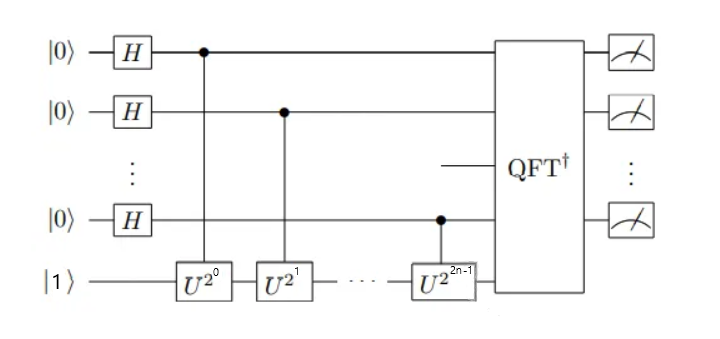
\includegraphics[width=\columnwidth]{shor_n_qubit.png}
    \caption{QPE für Shor~\cite{anonymousket}}
    \label{fig:shor_n_qubit}
  \end{figure}

Die Realisierung der Transformation erfordert die Implementierung einiger arithmetischer Operationen in Quantenschaltkreisform. 
Diese fungieren als Bausteine, die zusammengesetzt zur Konstruktion des übergeordneten Quantenschaltkreises für die modulare Multiplikation beitragen. 
Zu den erforderlichen arithmetischen Operationen gehört die Addition, Subtraktion sowie die modulare Addition.

In den folgenden Abschnitten werden die untergeordneten arithmetischen Operationen bis hin zur modularen Multiplikation implementiert.

\subsubsection{Addition} \label{sec:QuantumAdder}
Der Quantenschaltkreis für die Addition bildet das Fundament der \(U\)-Gatter und 
stellt einen der am häufigsten verwendeten Bausteine dar. 
Deswegen hat die Implementierung der Addition einen erheblichen Einfluss auf den Ressourcenbedarf des gesamten Quantenalgorithmus
und sollte daher möglichst effizient umgesetzt werden.

Eine Möglichkeit, die Addition als Quantenschaltkreis zu realisieren, 
besteht im Nachbau eines klassischen Schaltkreises aus Volladierern. 
Da es nicht möglich ist, 
die notwendigen klassischen Gatter wie AND und OR als unitäre Transformation mit nur zwei Qubits darzustellen~\cite{Hoever2023QC},
werden zusätzliche Hilfsqubits benötigt.
Die zusätzlichen Hilfsqubits bewirken, dass der Nachbau eines klassischen Schaltkreises für die Addition zweier \(n\)-Bit Zahlen, 
also solche der Größenordnung \(2^n\), mindestens \(3n\) Qubits benötigt~\cite{zalka1998fast}.

Eine effizientere Methode, welche ohne Hilfsqubits auskommt, ist die Quanten"=Addition~\cite{draper2000addition}. 
Die Quanten-Addition führt die Berechnung auf quantenmechanische Weise durch. 
Im Wesentlichen wird dabei die Addition in der Fourierbasis berechnet. 
Dafür befindet sich ein Summand des Quantenregisters \(\ket{b}_n\) in der Standardbasis und 
der andere Summand des Quantenregisters \(\ket{a}_n\) in der Fourierbasis.
Da sich das zweite Quantenregister in der Fourierbasis \(\Phi\) befindet, 
wird dieses als \(\ket{\Phi(a)}_n\) bezeichnet.
Anschließend kontrolliert der Summand in \(\ket{b}_n\) kontrollierte Phasen-Gatter, 
die auf den anderen Summanden in \(\ket{\Phi(a)}_n\) wirken.
Die durch die kontrollierten Phasen-Gatter induzierten Phasenverschiebungen übertragen die Werte, 
die dem Zustand des Summanden \(\ket{b}_n\) in der Fourierbasis entsprechen.
Dadurch befindet sich anschließend in dem Zielregister der Phasen-Gatter die Addition beider Werte in der Fourierbasis mit \(\ket{\Phi(a+b)}_n\).

Im Folgenden wird ein Beispiel für die Quanten-Addition zweier Quantenregister \(\ket{a}_3\) und \(\ket{b}_3\) betrachtet:
\begin{figure}[H]
    \centering
    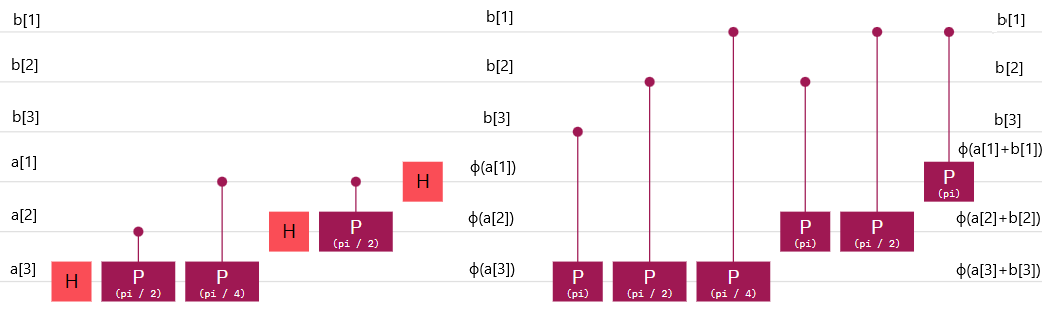
\includegraphics[width=\columnwidth]{3_qubit_quantum_add.png}
    \caption{Quantum-Addition}
    \label{fig:3_qubit_quantum_add}
  \end{figure}
Die Registermarkierungen in der Mitte von Abbildung~\ref{fig:3_qubit_quantum_add} unterteilen die Darstellung in zwei Hälften.
Die linke Hälfte repräsentiert die Quanten-Fourier-Transformation, 
während die rechte Hälfte die Quanten-Addition zeigt.

Wie man an der Struktur der Quanten-Addition erkennen kann,
ist die Anordnung der Gatter fast identisch mit der Quanten-Fourier-Transformation.
Ein Unterschied besteht darin, 
dass die Hadamard-Gatter durch kontrollierte \(P(\pi)\) Phasen-Gatter ersetzt wurden.
Sowohl das Hadamard-Gatter als auch das \(P(\pi)\) Phasen-Gatter erzeugt eine relative Phase von \(e^{\pi i}\).
Ein weiterer Unterschied zur Quanten-Fourier-Transformation besteht darin, 
dass die kontrollierten Phasen-Gatter nicht durch das Quantenregister kontrolliert werden, 
auf das die Gatter auch wirken.
Stattdessen kontrollieren die Qubits des Quantenregisters \(\ket{b}_3\) die Phasen-Gatter, 
welche auf das \(\ket{a}_3\) Quantenregister wirken.
Dabei wird das \(P(\pi)\) Phasen-Gatter durch das Qubit, des Quantenregisters \(\ket{b}_3\) kontrolliert,
welches die gleiche Wertigkeit hat wie das Zielqubit des Quantenregisters \(\ket{a}_3\).
Jedes weitere kontrollierte Phasen-Gatter für das gleiche Zielqubit 
wird fortlaufend von dem nächstkleineren Qubit des Quantenregisters \(\ket{b}_3\) kontrolliert.

Im Prinzip handelt es sich bei dieser Quantenschaltung um eine Anwendung derselben Phasenverschiebungen 
wie bei der Quanten-Fourier-Transformation. 
Der grundlegende Unterschied liegt darin, 
dass diese Phasenverschiebungen kontrolliert auf ein anderes Quantenregister angewendet werden.

Die Wirkung der Quanten-Addition wird anhand der Abbildung~\ref{fig:3_qubit_quantum_add} verdeutlicht.
Zu Beginn der linken Hälfte befinden sich beide Quantenregister in der Standardbasis.
Auf das Zielregister \(\ket{a}_3\) wird die Quanten-Fourier-Transformation ohne Swap-Gatter angewendet.
Dadurch befindet sich \(\ket{a}_3\) nun in der Fourierbasis \(\Phi\), also \(\ket{\Phi(a)}_3\):
\begin{align*}
  \begin{aligned}
  &\ket{\Phi(a)}_3 =\\
  &\frac{1}{\sqrt{8}} \Bigg[ \Big(\ket{0} + { e^{\frac{2 \pi i (2^0a_1)}{2^1}}}\ket{1} \Big) \tensor
  \Big(\ket{0} + { e^{\frac{2 \pi i (2^1a_2+2^0a_1)}{2^2}}}\ket{1} \Big) \tensor
  \Big(\ket{0} + { e^{\frac{2 \pi i (2^{2}a_3 +2^1a_2+2^0a_1)}{2^3}}}\ket{1} \Big) \Bigg]
  \end{aligned}
\end{align*}
Anschließend wird auf das hinterste Tensorprodukt ein \(P(\pi)\) Phasen-Gatter angewendet,
das von \(\ket{b_3}_1\) kontrolliert wird.
Wenn sich Qubit \(\ket{b_3}_1\) im Zustand \(\ket{0}\) befindet, passiert nichts.
Befindet es sich jedoch im Zustand \(\ket{1}\), wird die Phasenverschiebung des Phasen-Gatters angewendet.
Dieses Verhalten lässt sich für beide Fälle mit den entsprechenden Matrizen
\begin{align*}
  \begin{pmatrix}
    1 & 0 \\
    0 & e^{\pi i b_3}
  \end{pmatrix}  
  \text{beziehungsweise}  
  \begin{pmatrix}
    1 & 0 \\
    0 & e^{\frac{2\pi i (2^2b_3)}{2^3}}
  \end{pmatrix}
\end{align*}
beschreiben.
Schreibt man das hinterste Tensorprodukt als Vektor, ergibt sich die folgende Formulierung:
\[\frac{1}{\sqrt{2}}( \ket{0} + { e^{\frac{2 \pi i (2^{2}a_3 +2^1a_2+2^0a_1)}{2^3}}}\ket{1}) =
\frac{1}{\sqrt{2}}
\begin{pmatrix}
     1  \\
     e^{\frac{2 \pi i (2^{2}a_3 +2^1a_2+2^0a_1)}{2^3}}
  \end{pmatrix}
    \]
Dann wird durch das Ergebnis der Verrechnung mit dem Phasen-Gatter deutlich, 
dass die Addition im Wesentlichen in der Phase des Quantenzustands stattfindet:
\[\begin{pmatrix}
    1 & 0 \\
    0 & e^{\frac{2\pi i (2^2b_3)}{2^3}}
  \end{pmatrix}
    \cdot
\frac{1}{\sqrt{2}}
\begin{pmatrix}
    1  \\
     e^{\frac{2 \pi i (2^{2}a_3 +2^1a_2+2^0a_1)}{2^3}}
  \end{pmatrix}
  =
  \frac{1}{\sqrt{2}}
  \begin{pmatrix}
    1  \\
     e^{\frac{2 \pi i (2^{2}(a_3+b_3) +2^1a_2+2^0a_1)}{2^3}}
  \end{pmatrix}
\]
Wie in der Abbildung~\ref{fig:3_qubit_quantum_add} erkenntlich,
wirken auf das hinterste Tensorprodukt auch noch die beiden Phasen-Gatter \(P(\frac{\pi}{2})\) und \(P(\frac{\pi}{4})\) mit:
\begin{align*}
    P\left(\frac{\pi}{2}\right) &= 
\begin{pmatrix}
    1 & 0 \\
    0 & e^{\frac{\pi}{2} i b_2}
  \end{pmatrix}
  =
  \begin{pmatrix}
    1 & 0 \\
    0 & e^{\frac{2\pi i (2^1b_2)}{2^3}}
  \end{pmatrix} \\
P\left(\frac{\pi}{4}\right) &= 
\begin{pmatrix}
    1 & 0 \\
    0 & e^{\frac{\pi}{4} i b_1}
  \end{pmatrix}
  =
  \begin{pmatrix}
    1 & 0 \\
    0 & e^{\frac{2\pi i (2^0b_1)}{2^3}}
  \end{pmatrix}
\end{align*}
Multipliziert man beide von links an das vorherige Ergebnis erhält man:
\begin{align*}
    &\begin{pmatrix}
        1 & 0 \\
        0 & e^{\frac{2\pi i (2^0b_1)}{2^3}}
      \end{pmatrix}
      \cdot
      \begin{pmatrix}
        1 & 0 \\
        0 & e^{\frac{2\pi i (2^1b_2)}{2^3}}
      \end{pmatrix}
      \cdot
      \frac{1}{\sqrt{2}}
      \begin{pmatrix}
        1  \\
         e^{\frac{2 \pi i (2^{2}(a_3+b_3) +2^1a_2+2^0a_1)}{2^3}} 
      \end{pmatrix} 
     \\
      =&
      \frac{1}{\sqrt{2}}
      \begin{pmatrix}
        1  \\
         e^{\frac{2 \pi i (2^{2}(a_3+b_3) +2^1(a_2+b_2)+2^0(a_1+b_1))}{2^3}}
      \end{pmatrix}
\end{align*}
Wendet man alle weiteren Phasen-Gatter auf das vollständige Tensorprodukt an, 
wird dies zu:
\begin{align*}
    \frac{1}{\sqrt{8}} 
    \Bigg[ 
      \Big(\ket{0} + { e^{\frac{2 \pi i (2^0(a_1+b_1))}{2^1}}}\ket{1} \Big) 
      &\tensor
      \Big( \ket{0} + { e^{\frac{2 \pi i (2^1(a_2+b_2)+2^0(a_1+b_1))}{2^2}}}\ket{1} \Big)\\ 
      &\tensor
      \Big( \ket{0} + { e^{\frac{2 \pi i (2^{2}(a_3+b_3) +2^1(a_2+b_2)+2^0(a_1+b_1))}{2^3}}}\ket{1} \Big) 
    \Bigg]
\end{align*}
Setzt man in diese Formel zwei Zahlen in Binärschreibweise ein, 
wird man denselben Zustand erhalten,
als würde man die Summe der beiden Zahlen in die Formel der Quanten-Fourier-Transformation einsetzt.
Beispielsweise sei \(a = 3\) also binär \(a_3 = 0\), \(a_2 = 1\), \(a_1 = 1\) und 
\(b = 1\) also \(b_3 = 0\), \(b_2 = 0\), \(b_1 = 1\):
\begin{align*}
&\begin{aligned}\frac{1}{\sqrt{8}} 
\Bigg[ \Big(\ket{0} + { e^{\frac{2 \pi i (2^0(1+1))}{2^1}}}\ket{1} \Big) 
&\tensor
\Big( \ket{0} +  e^{\frac{2 \pi i (2^1(1+0)+2^0(1+1))}{2^2}}\ket{1} \Big) \\
&\tensor
\Big( \ket{0} +  e^{\frac{2 \pi i (2^{2}(0+0) +2^1(1+0)+2^0(1+1))}{2^3}}\ket{1} \Big) 
\Bigg]
\end{aligned}\\
=&\frac{1}{\sqrt{8}} 
\Bigg[ \Big(\ket{0} + \ket{1} \Big) \tensor
\Big( \ket{0} +   \ket{1} \Big) \tensor
\Big( \ket{0} +  e^{\pi i }\ket{1} \Big) 
\Bigg]
\end{align*}
Dass dies tatsächlich der Summe in der Fourierbasis entspricht, wird deutlich, 
wenn man das gleiche Tensorprodukt im Kontext der Quanten-Fourier-Transformation bildet:
\begin{align*}
    QFT(\ket{c}_3) = 
    \frac{1}{\sqrt{8}} 
    \Bigg[ \Big(\ket{0} + { e^{\frac{2 \pi i (2^0(c_1))}{2^1}}}\ket{1} \Big) 
    &\tensor
    \Big( \ket{0} + e^{\frac{2 \pi i (2^1(c_2)+2^0(c_1))}{2^2}}\ket{1} \Big) \\
    &\tensor
    \Big( \ket{0} + { e^{\frac{2 \pi i (2^{2}(c_3) +2^1(c_2)+2^0(c_1))}{2^3}}}\ket{1} \Big) 
\Bigg]
\end{align*}
Die Summe von \(a\) und \(b\) entspricht \(c = 4\) also \(c_3 = 1,~c_2 = 0,~c_1=0\):
\begin{align*}
    QFT(\ket{4}_3) &=
    \begin{aligned}[t]
      \frac{1}{\sqrt{8}} \Bigg[ \Big(\ket{0} + { e^{\frac{2 \pi i (2^0(0))}{2^1}}}\ket{1} \Big) 
      &\tensor
      \Big( \ket{0} + { e^{\frac{2 \pi i (2^1(0)+2^0(0))}{2^2}}}\ket{1} \Big) \\
      &\tensor
      \Big( \ket{0} + { e^{\frac{2 \pi i (2^{2}(1) +2^1(0)+2^0(0))}{2^3}}}\ket{1} \Big) \Bigg]
    \end{aligned} \\
    &= 
    \frac{1}{\sqrt{8}} \Bigg[ \Big(\ket{0} + { e^{\frac{2 \pi i (0)}{2^1}}}\ket{1} \Big) 
    \tensor
    \Big( \ket{0} + { e^{\frac{2 \pi i (0)}{2^2}}}\ket{1} \Big) 
    \tensor
    \Big( \ket{0} + { e^{\frac{2 \pi i (2^{2}(1))}{2^3}}}\ket{1} \Big) \Bigg] \\
    &=\frac{1}{\sqrt{8}} \Bigg[ \Big(\ket{0} + \ket{1} \Big) 
    \tensor
    \Big( \ket{0} +   \ket{1} \Big) 
    \tensor
    \Big( \ket{0} +  e^{\pi i }\ket{1} \Big) \Bigg]
\end{align*}
Der Zustand, 
der durch die Quanten-Addition der Summanden \(a=3\) und 
\(b=1\) in zwei verschiedenen Quantenregistern mit jeweils drei Qubits erzeugt wird, 
entspricht dem Zustand, der entsteht, 
wenn man die Quanten-Fourier-Transformation auf ein Quantenregister mit drei Qubits anwendet, 
das die Summe der beiden Zahlen enthält.

Mit einer anschließenden inversen Quanten-Fourier-Transformation 
kann die Summe in die Standardbasis und somit in einen messbaren Zustand transformiert werden:
\[
iQFT(\ket{\Phi(4)_3})
=
 iQFT \Bigg(\frac{1}{\sqrt{8}} \Big[ (\ket{0} + \ket{1} ) \tensor
( \ket{0} +   \ket{1} ) \tensor
( \ket{0} +  e^{\pi i }\ket{1} ) \Big]\Bigg) 
=
\ket{4}_3
\]

Das Zielregister sollte aus genügend Qubits bestehen, 
damit die Summe vollständig erfasst werden kann.
Andernfalls kommt es zum Overflow mit \(a + b \bmod 2^n\), 
wobei \(n\) die Anzahl der Qubits des Zielregisters beschreibt.

Für die Realisierung der modularen Multiplikation wird zu keinem Zeitpunkt der Berechnung eine Addition zweier Zwischenergebnisse benötigt. 
Genauer gesagt, ist es nicht nötig, ein Quantenregister auf ein anderes zu addieren. 
Stattdessen wird die Quanten-Addition benutzt, um eine vorab bekannte Zahl auf ein Quantenregister zu addieren.

Bei der Quanten-Addition mit zwei Quantenregistern, 
wie in Abbildung~\ref{fig:3_qubit_quantum_add} erfolgt die Phasenverschiebung kontrolliert,  
also in Abhängigkeit des Inhaltes von Quantenregister \(\ket{b}_3\).
Ist der Inhalt von Quantenregister \(\ket{b}_3\) vorab bekannt,
können gewöhnliche Phasen-Gatter anstelle von kontrollierten verwendet werden~\cite{beauregard2003circuit}.

Wenn bei der Quanten-Addition mit zwei Quantenregistern ein Phasen-Gatter aufgrund des zugehörigen Kontrollqubits im Zustand \(\ket{1}\) angewendet wird,
wird es in der Variante mit einem einzelnen Quantenregister als gewöhnliches Phasen-Gatter verwendet.
Ist das Kontrollqubit hingegen im Zustand \(\ket{0}\), 
wodurch das Phasen-Gatter bei der Quanten-Addition mit zwei Quantenregistern nicht zur Anwendung kommt, 
wird dieses Phasen-Gatter in der Variante mit nur einem Quantenregister weggelassen.

\begin{figure}[H]
  \centering
  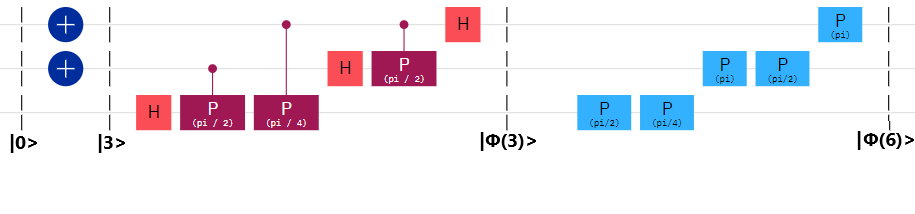
\includegraphics[width=\columnwidth]{3_qubit_fixed_quantum_addition.png}
  \caption{Quantum-Addition fixierte Phasenverschiebungen}
  \label{fig:3_qubit_fixed_quantum_addition}
\end{figure}
In Abbildung~\ref{fig:3_qubit_fixed_quantum_addition} ist die Quanten-Addition für ein 3-Qubit Quantenregister abgebildet.
Die blauen Phasen-Gatter sorgen für die Quanten-Addition mit einem fixierten Wert von \(3\).
Vergleicht man Abbildung~\ref{fig:3_qubit_fixed_quantum_addition} mit Abbildung~\ref{fig:3_qubit_quantum_add} fällt auf, 
dass das allererste Phasen-Gatter der Quanten-Addition nicht vorkommt.
Im Quantenschaltkreis der Abbildung~\ref{fig:3_qubit_quantum_add} würde ein Registerinhalt von \(b = 3\) das Kontrollqubit \(b_3\) nicht setzen. 
Somit kommt das erste Phasen-Gatter der Quanten-Addition nicht zum Einsatz und 
wird deswegen in der Variante wie in Abbildung~\ref{fig:3_qubit_fixed_quantum_addition} weggelassen. 

Des Weiteren ist es möglich, 
den Quantenschaltkreis der Quanten-Addition für eine vorab festgelegte Zahl ressourcensparender zu realisieren.
Die Optimierung bezieht sich dabei auf die Anzahl der verwendeten Gatter.
Wird die Quanten-Addition für eine feste Zahl realisiert, 
können für jedes einzelne Qubit die angewendeten Phasenverschiebungen vorab zusammengerechnet werden.
Demnach bietet es sich an, 
die zusammengerechneten Phasenverschiebungen in ein einzelnes Phasen-Gatter zusammenzufassen.
Nach diesem Prinzip benötigt man für eine Quanten-Addition maximal ein einzelnes Phasen-Gatter pro Qubit.

\begin{figure}[H]
  \centering
  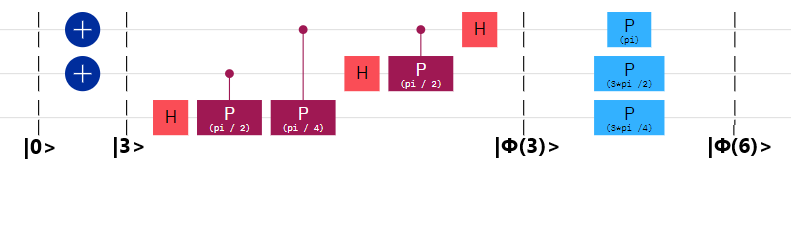
\includegraphics[width=\columnwidth]{3_qubit_fixed_quantum_addition_opt.png}
  \caption{Ressourcensparende Quantum-Addition}
  \label{fig:3_qubit_fixed_quantum_addition_opt}
\end{figure}
Der Quantenschaltkreis in Abbildung~\ref{fig:3_qubit_fixed_quantum_addition_opt} führt die identische 
Berechnung durch wie der Quantenschaltkreis aus Abbildung~\ref{fig:3_qubit_fixed_quantum_addition}.
Darüber hinaus werden die benötigten Phasenverschiebungen mit einem einzigen Phasen-Gatter pro Qubit realisiert.

Die Implementierung nutzt die ressourceneffiziente Variante der Quanten-Addition.
In der Funktion \mintinline{python}{A_Gate} wird ein Gatter erzeugt, 
das sämtliche für die Quanten-Addition erforderlichen Phasen-Gatter umfasst.
Der Code zur Funktion ist in Abbildung~\ref{code:QuantumAdd} dargestellt.
\begin{listing}[H]
\begin{minted}[linenos,fontsize=\footnotesize]{python}    
def A_Gate(a_bin: list[int]) -> qiskit.circuit.gate:
    A_Gate = qiskit.QuantumCircuit(len(a_bin))
    theta_list = [0.0]*len(a_bin)
    for target_bit in range(len(a_bin)):
        exponent = 1
        for control_bit in reversed(range(target_bit+1)):
            if a_bin[control_bit] == 1:
                theta_list[target_bit]+= 2*pi/(2**(exponent))
            exponent+=1
    for qubit_index in range(len(a_bin)):
        A_Gate.append(P_Gate(theta_list[qubit_index]),[qubit_index])
    A_Gate = A_Gate.to_gate()
    A_Gate.name = " Add(" + str (binToDez(a_bin) )+ ")"
    return A_Gate 
  \end{minted}
  \caption{Quantum-Addition in Qiskit}
  \label{code:QuantumAdd}
\end{listing}
Der Funktion \mintinline{python}{A_Gate} wird der zu addierende Summand im Binärformat übergeben, 
wobei am Index Null das Least-Significant-Bit liegt.
Abhängig von der Anzahl der Bits des Summanden wird ein Quantenschaltkreis mit der gleichen Anzahl an Qubits erzeugt. 
In den Zeilen 4 bis 9 werden die Phasenverschiebungen, die auf ein einzelnes Qubit wirken sollen, berechnet und akkumuliert.
Anschließend wird in den Zeilen 10 bis 11 auf jedes Qubit des Quantenschaltkreises ein individuelles Phasen-Gatter angewendet.
Die Phasenverschiebung eines einzelnen Phasen-Gatters ergibt sich aus der vorherigen Akkumulation in den Zeilen 4 bis 9.
Abschließend wird der Quantenschaltkreis in ein Gatter umgewandelt und mit einer passenden Bezeichnung versehen.

\subsubsection{Subtraktion}
Die Quanten-Addition besteht ausschließlich aus unitären Gattern und ist daher selbst ebenfalls unitär.
Diese Eigenschaft vereinfacht die Implementierung der Subtraktion. 
Durch die Invertierung der Quanten-Addition ergibt sich ein Quantenschaltkreis, 
der eine Subtraktion in der Fourierbasis ausführt. 
Damit erhält man praktisch einen Quantenschaltkreis, für die Quanten-Subtraktion.

Genau wie bei der Quanten-Addition kann es auch bei der Quanten-Subtraktion zu einem Overflow
oder im konkreten Kontext zu einem Underflow kommen.
Dieser Effekt tritt ein, 
falls der im Zielregister befindliche Minuend kleiner ist als der Subtrahend.

Der Effekt des Underflows wird verwendet, um herauszufinden, 
ob der Subtrahend größer als der Minuend ist.
Angenommen, man hat zwei Zahlen, 
die maximal der Größenordnung \(2^n\) entsprechen und 
ein Zielregister, 
welches aus \(n+1\) Qubits besteht.
Der Minuend \(b\) befindet sich im Zielregister, 
also \(\ket{\Phi(b)}_{n+1}\), 
worauf die Quanten-Subtraktion mit dem Subtrahenden \(a\) wirkt.
Dann existieren zwei mögliche Fälle~\cite{beauregard2003circuit}:
\[b \geq a\;\rightarrow\;\ket{\Phi(b-a)}_{n+1};\quad
b < a \;\rightarrow\;\ket{\Phi(2^{n+1}-(a-b))}_{n+1}
  \]
Das Most-Significant Bit ist ausschließlich im zweiten Fall gesetzt und kann somit, 
nachdem das Quantenregister in die Standardbasis transformiert wurde, 
als eine Art Borrow-Bit verwendet werden.

Die Implementierung der Quanten-Subtraktion ist aufgrund der \mintinline{python}{inverse} Funktion von Qiskit unkompliziert.
Wendet man die \mintinline{python}{inverse} Funktion auf ein Gatter der Quanten-Addition aus der \mintinline{python}{A_Gate} Funktion an, 
wird dieses in die Quanten-Subtraktion invertiert.
Der zugehörige Code ist in~\ref{code:QuantumSub} abgebildet.
\begin{listing}[H]
\begin{minted}[linenos,fontsize=\footnotesize]{python}    
def S_Gate(subtrahend_bin: list[int]) -> qiskit.circuit.gate:
    S_Gate = A_Gate(subtrahend_bin).inverse()
    S_Gate.name = "  Sub(" + str (binToDez(subtrahend_bin) )+ ")"
    return S_Gate
  \end{minted}
  \caption{Quantum-Subtraktion in Qiskit}
  \label{code:QuantumSub}
\end{listing}

\subsubsection{Modulare Addition} \label{sub:modulareAddition}
Das Gatter der Quanten-Addition und der Quanten-Subtraktion ermöglichen die Konstruktion einer unitären Transformation, 
welche die Berechnung der modularen Addition realisiert.
Gemeinsam bilden sie einen Quantenschaltkreis, 
der das Ergebnis der Berechnung \(\ket{\Phi(a+b)\bmod N}\) für \(a, b < N\) im Zielregister speichert.

\begin{figure}[H]
  \centering
  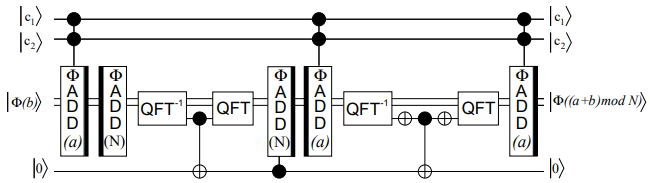
\includegraphics[width=\columnwidth]{Modular_adder_Paper.PNG}
  \caption{Modulare Addition nach Beauregard~\cite{beauregard2003circuit}}
  \label{fig:modulare_addition_paper}
\end{figure}
Abbildung~\ref{fig:modulare_addition_paper} zeigt das Konzept, 
das als Bauplan für die Implementierung der modularen Addition diente.
In der Grafik sind zwei Arten von \(\Phi \ADD\)-Gattern zu sehen:
Die Quanten-Addition, erkennbar an dem fettgedruckten Strich auf der rechten Seite 
und die Quanten-Subtraktion, erkennbar an dem fettgedruckten Strich auf der linken Seite.
Sowohl die Quanten-Addition als auch die Quanten-Subtraktion addieren beziehungsweise subtrahieren eine feste Zahl und 
sind somit die zuvor vorgestellten Varianten mit gewöhnlichen Phasen-Gattern.

Der Quantenschaltkreis zur modularen Addition agiert als Baustein in einem größeren Gesamtbild. 
Aus diesem Grund werden zwei Kontrollqubits \(\ket{c_1}_1\) und \(\ket{c_2}_1\) eingebaut, 
die im weiteren Verlauf Anwendung finden.
Das Eingaberegister, das zugleich als Zielregister dient,  
ist initial bereits in der Fourierbasis mit \(\ket{\Phi(b)}\).

Das Zielregister wird um ein weiteres Qubit erweitert, 
welches das Most-Significant-Bit des Zielregisters darstellt.
Dieses Qubit hat einen besonderen Anwendungszweck und wird im Weiteren als Borrow-Qubit bezeichnet.
Insgesamt besteht das Zielregister also aus \(n+1\) Qubits, 
wenn der Modulus \(N\) einer Größenordnung von \(2^n\) entspricht.
Alle nachhaltigen Veränderungen durch den Quantenschaltkreis betreffen ausschließlich das Zielregister.
Darüber hinaus verwendet die Quantenschaltung ein weiteres Qubit, 
welches initial im Zustand \(\ket{0}\) ist.
Der Zustand dieses einzelnen Qubits bedingt eine Fallunterscheidung in der Berechnung des Quantenschaltkreises und 
wird daher im Weiteren als Bedingungs-Qubit bezeichnet. 

Um die Berechnung des Quantenschaltkreises nachvollziehen zu können, 
werden die Auswirkungen der verwendeten Gatter im Einzelnen erklärt.
Die erste Quanten-Addition sorgt dafür, 
dass auf das initiale Zielregister \(\ket{\Phi(b)}\) eine Addition mit \(a\) angewendet wird und 
dadurch \(\ket{\Phi(b + a)}\) entspricht.
Darauf folgt eine Quanten-Subtraktion, 
die mit dem Subtrahend \(N\) auf das Zielregister \(\ket{\Phi(b + a)}\) wirkt und 
dieses in den Zustand \(\ket{\Phi(b + a - N)}\) überführt. 
Daraus resultieren zwei mögliche Zustände:
\[1.~(b+a) \geq N~\rightarrow~\ket{\Phi((b+a) - N)}_{n+1}\]
\[2.~
(b+a) < N~\rightarrow~\ket{\Phi(2^{n+1}-(N-(a+b)))}_{n+1}
  \]
Im ersten Fall entspricht das Ergebnis der korrekten Berechnung von \(a+b \bmod N\).
In diesem Fall ist der Inhalt des Quantenregisters mit \(a+b \bmod N\) kleiner als \(N\), 
weshalb das Borrow-Bit nicht gesetzt ist.
Im Gegensatz dazu ist das Ergebnis im zweiten Fall fehlerhaft.
Da bei \((b+a) < N\) bereits der Rest der modularen Restklasse im Register steht, 
wird durch die Quanten-Subtraktion ein \(N\) zu viel vom Registerinhalt abgezogen.
Dadurch entsteht ein Underflow im Zielregister, 
wodurch das Borrow-Bit gesetzt wird.

Als Nächstes wirkt die inverse Quanten-Fourier-Transformation auf das Zielregister und 
führt eine Transformation in die Standardbasis durch.
Aufgrund des Basiswechsels in die Standardbasis beschreiben die Zustände der Qubits des Zielregisters nun das Ergebnis in der Binärdarstellung.
Im ersten Fall befindet sich das Borrow-Bit im Zustand \(\ket{0}\) und im zweiten Fall im Zustand \(\ket{1}\).
Anhand dieser Unterscheidung kann man eine bedingte Operation mittels eines kontrollierten X-Gatters realisieren.
Dafür kontrolliert das Borrow-Bit ein X-Gatter, 
welches auf das Bedingungs-Qubit wirkt.
Dadurch wird das Bedingungs-Qubit ausschließlich im zweiten Fall in den Zustand \(\ket{1}\) versetzt.
Danach wird das Zielregister wieder in die Fourierbasis transformiert, 
indem die Quanten-Fourier-Transformation angewendet wird.
Anschließend kontrolliert das Bedingungs-Qubit eine Quanten-Addition mit dem Summanden \(N\) auf das Zielregister.
Die kontrollierte Quanten-Addition wird also nur im zweiten Fall angewendet und korrigiert das vorher ungültige Ergebnis
zu dem korrekten:
\[
\ket{\Phi(2^{n+1}-(N-(a+b)))}_{n+1} \underrightarrow{~+N~} 
\ket{\Phi(2^{n+1}+(a+b))}_{n+1} \underrightarrow{\text{overflow }2^{n+1}}
\ket{\Phi(a+b)}_{n+1}
  \]
Nun befindet sich in beiden Fällen das korrekt berechnete Ergebnis im Zielregister mit \(\ket{\Phi(a+b)\bmod N}\).
Somit ist die Berechnung der modularen Addition abgeschlossen.

Je nachdem, welcher der beiden Fälle eingetreten ist, 
befindet sich das Bedingungs-Qubit in einem anderen Zustand.
Um zu verhindern, dass sich das Bedingungs-Qubit in einem ungewissen Zustand befindet und dadurch zum "`Trash"'-Qubit wird, 
wird der initiale Zustand \(\ket{0}\) des Bedingungs-Qubit durch die restlichen Gatter des Quantenschaltkreises wiederhergestellt.
Ein eindeutiger Zustand ermöglicht, dass das Bedingungs-Qubit bei weiteren Berechnungen wiederverwendet werden kann.

Um das Bedingungs-Qubit zurückzusetzen, 
wird zuerst eine Quanten-Subtraktion mit \(a\) auf das Zielregister angewendet.
Um die Auswirkungen dieser Quanten-Subtraktion hervorzuheben, wird der Registerinhalt für beide Fälle untersucht:
Im ersten Fall war \((b+a) \geq N\) weswegen die Subtraktion von \(N\) zum Ergebnis der modularen Addition führte.
Da \(a, b < N\) gilt, ist das Ergebnis der modularen Addition kleiner als \(a\).
Die Quanten-Subtraktion mit \(a\) führt also zu einem Underflow, wodurch das Borrow-Bit gesetzt wird.
Im zweiten Fall war \((b+a) < N\).
Deswegen wurde die Subtraktion von \(N\) nicht durchgeführt, 
beziehungsweise wieder rückgängig gemacht, da \((b+a)\) bereits das Ergebnis der modularen Addition ist.
Für den zweiten Fall gilt als Ergebnis also \((b+a)\).
Dies ist nicht kleiner als \(a\), 
darum kommt es zu keinem Underflow und das Borrow-Bit wird deswegen nicht gesetzt.
Der Zustand des Borrow-Bits ist nun also im Vergleich zu den Fällen des vorherigen Abschnitts der Quantenschaltung invertiert.

Um das Borrow-Bit auslesen zu können, 
wird analog zum vorherigen Abschnitt des Quantenschaltkreises eine inverse Quanten-Fourier-Transformation durchgeführt.
Anschließend wird ein X-Gatter auf das Borrow-Bit angewendet.
Dadurch befindet sich das Borrow-Bit nun in denselben Zuständen wie in den beiden Fällen des ersten Abschnitts der Quantenschaltung.
Im nächsten Schritt kontrolliert das Borrow-Bit ein X-Gatter, das auf das Bedingungs-Qubit wirkt.
Dadurch wird es wieder in den initialen Zustand \(\ket{0}\) versetzt.

Um den Zustand \(\ket{\Phi(a+b)\bmod N}\) des Zielregisters wiederherzustellen, 
werden die Gatter bis zur Quanten-Subtraktion mit \(a\)
nun in umgekehrter Reihenfolge und invers angewendet.
Zunächst wird ein selbstinverses X-Gatter auf das Borrow-Bit angewendet.
Danach folgt die Quanten-Fourier-Transformation, 
die quasi die Inverse der inversen Quanten-Fourier-Transformation darstellt.
Abschließend folgt die Quanten-Addition mit \(a\), 
um die zuvor erfolgte Quanten-Subtraktion von \(a\) auf das Zielregister zu revertieren.

Das Zielregister beinhaltet nun den gewünschten Zustand:
\[\ket{\Phi(a+b)\bmod N} \text{ für } a, b < N\]
Des Weiteren befindet sich das Bedingungs-Qubit wieder im initialen Zustand \(\ket{0}\) und kann für weitere Rechnungen wiederverwendet werden.

\bigskip

Wenn man den Quantenschaltkreis in Abbildung~\ref{fig:modulare_addition_paper} betrachtet,
fällt auf, 
dass nicht alle Quanten-Additionen und Quanten-Subtraktionen kontrolliert durchgeführt werden.
Die modulare Addition soll nur dann ausgeführt werden, 
wenn die Kontrollqubits \(\ket{c_1}_1\) und \(\ket{c_2}_1\) gesetzt sind.

Betrachtet man ausschließlich die kombinierte Wirkung der Gatter des Quantenschaltkreises, 
welche nicht von \(\ket{c_1}\) und \(\ket{c_2}\) kontrolliert sind, 
führen diese lediglich die Identitätstransformation durch~\cite{beauregard2003circuit}.
Dies liegt daran, dass keine modulare Addition mit \(a\) durchgeführt werden soll, 
wenn \(\ket{c_1}\) oder \(\ket{c_2}\) im Zustand \(\ket{0}\) ist. 
Aufgrund der Bedingung \(b < N\), 
steht bereits der modulare Rest im Zielregister und somit ist keine Berechnung notwendig.

Der Grund, weshalb nicht alle Quanten-Additionen, 
Quanten-Subtraktionen und gegebenenfalls sogar die (inversen) Quanten-Fourier-Transformationen kontrolliert sind,
liegt in der erhöhten Komplexität, die dadurch im Quantenschaltkreis entstehen würde~\cite{beauregard2003circuit}.
Wenn ein Kontrollqubit nicht aktiviert ist, wird das kontrollierte Gatter trotzdem ausgeführt, jedoch ohne praktische Wirkung.
Abbildung~\ref{fig:gatedef_U1U2U3_CNOT} zeigt die physikalische Implementierung dreier Single-Qubit-Gatter im Vergleich zu einem kontrollierten X-Gatter.
Wie in der Abbildung erkennbar, 
benötigt das kontrollierte Gatter mehr Hardware-Elemente als die drei Single-Qubit-Gatter.
Somit ist es nicht möglich, 
die Komplexität des Quantenschaltkreises zu verringern, 
indem zusätzliche Gatter kontrolliert angewendet werden.

\begin{figure}[H]
  \centering
  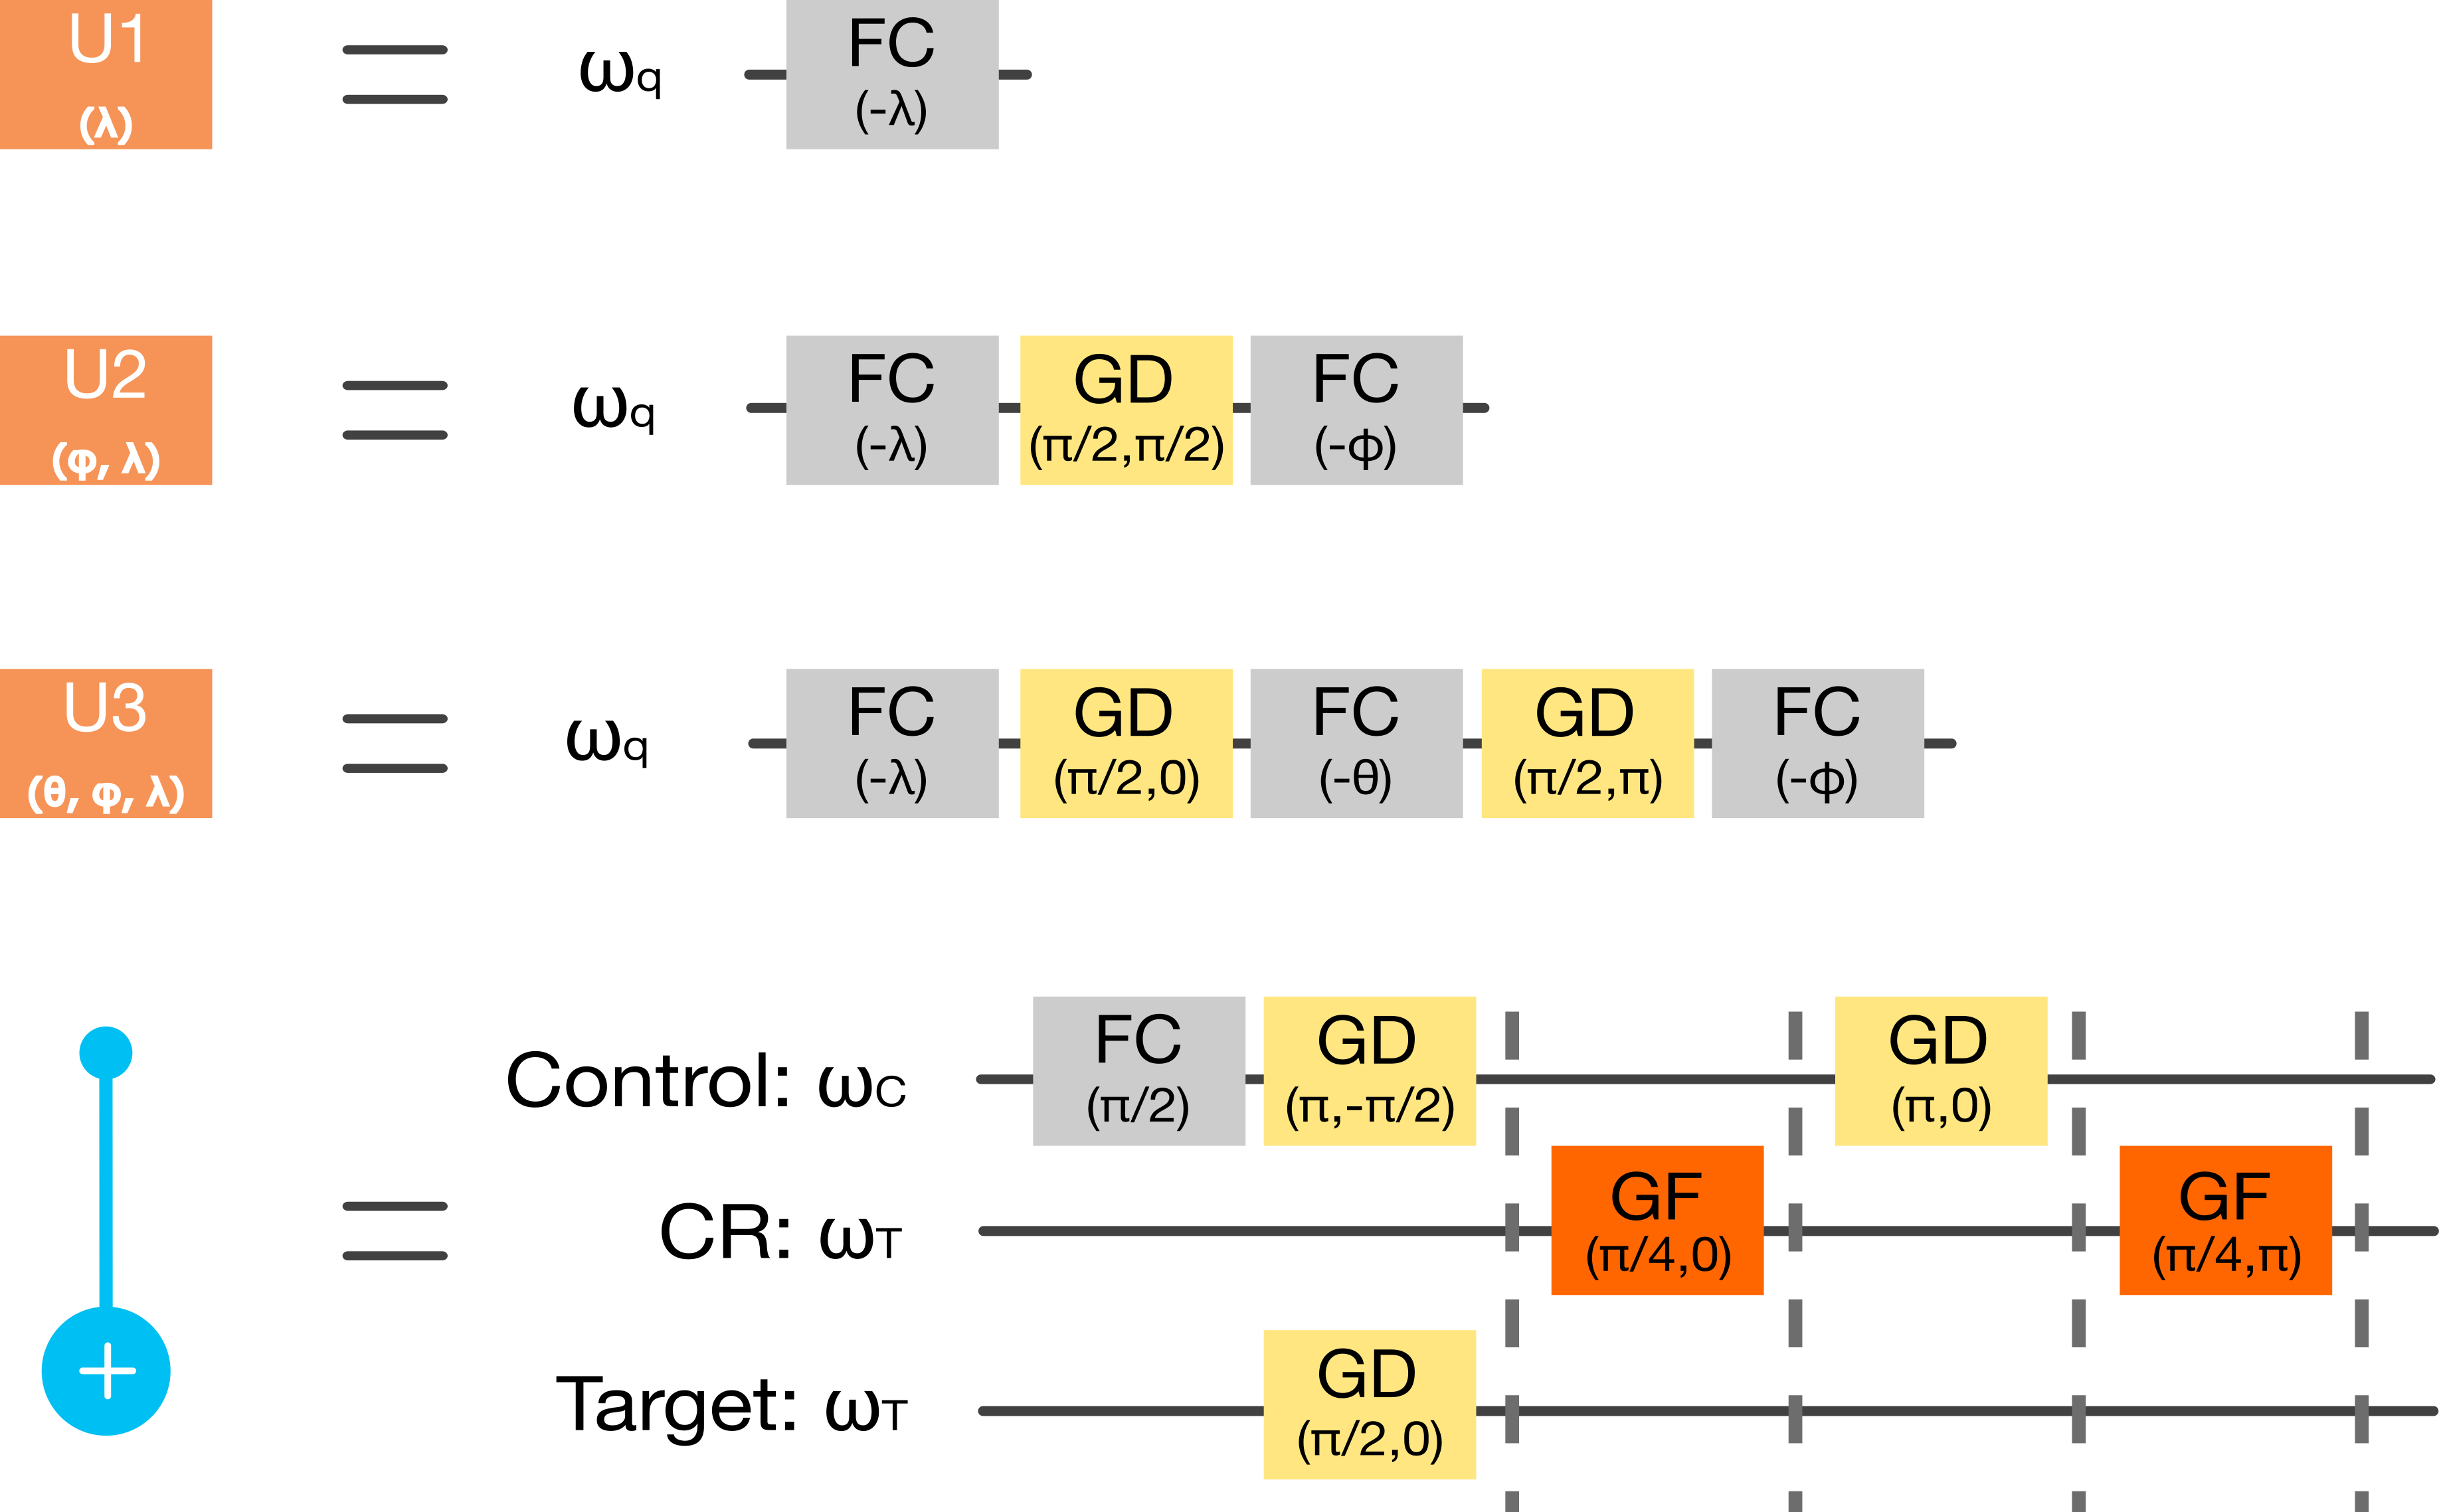
\includegraphics[scale=0.5]{gatedef_U1U2U3_CNOT.png}
  \caption{Physikalische Implementierung~\cite{ibmqx5}}
  \label{fig:gatedef_U1U2U3_CNOT}
\end{figure}

Ein weiterer Aspekt, 
der die Komplexität der Quantenschaltung für die modulare Addition erhöht, 
ist der Abschnitt, der das Bedingungs-Qubit zurücksetzt.
Wäre es möglich, diesen Teil auszulassen, könnten zwei der insgesamt fünf Quanten-Additionen bzw. 
Quanten-Subtraktionen sowie die Hälfte der (inversen) Quanten-Fourier-Transformationen eingespart werden.

Es gibt die Möglichkeit, bei einem Qubit einen Reset durchzuführen, wodurch dieses den Zustand \(\ket{0}\) annimmt.
In Qiskit kann dies mit der Funktion \mintinline{python}{Reset} realisiert werden~\cite{qiskitReset}.
Die Verwendung ist jedoch nicht zielführend, da diese durch keine unitäre Abbildungsmatrix
beschrieben werden kann.
Somit ist die Reset-Transformation nicht unitär und würde deswegen dazu führen, dass alle Quantenalgorithmen, 
die diese Funktion nutzen, ebenfalls nicht mehr unitär wären.
Da die Quantum-Phase-Estimation den Eigenwert einer \emph{unitären} Transformation extrahiert, 
ist diese Funktion für die Anwendung im Shor-Algorithmus ungeeignet.

\begin{figure}[H]
  \centering
  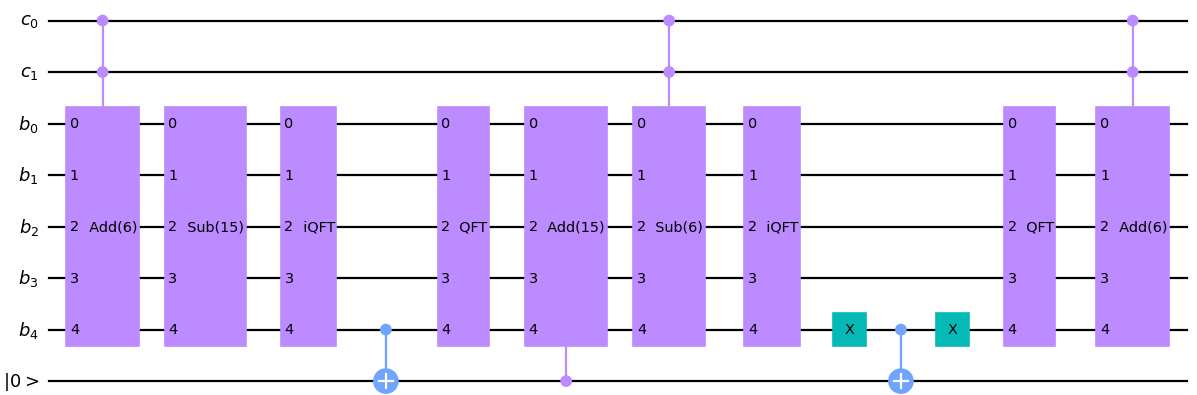
\includegraphics[width=\columnwidth]{modulareAddition.png}
  \caption{Qiskit modulare Addition}
  \label{fig:ModularAddition}
\end{figure}

Abbildung~\ref{fig:ModularAddition} zeigt die Implementierung eines Gatters für die modulare Addition 
mit \(a = 6\) und \(N = 15\) in Qiskit.
Der zugehörige Code, der ein Gatter wie in Abbildung~\ref{fig:ModularAddition} generiert, 
ist in der Funktion \mintinline{python}{Modular_Adder_Gate}~\ref{code:ModularAddition} enthalten.

Die Funktion \mintinline{python}{Modular_Adder_Gate} erwartet den Summand \(a\) und die Zahl \(N\) als Parameter, 
jeweils in der Form einer Liste, 
welche die Zahl in Binärdarstellung beschreibt.
Dabei repräsentiert der erste Index beider Listen das Least-Significant-Bit.
Wenn \(N\) der Größenordnung \(2^n\) entspricht, 
müssen die Listen jeweils von der Länge \(n+1\) sein, 
wobei das Most-Significant-Bit immer \(0\) entspricht.

Die Funktion definiert drei Wertebereiche, die die Positionen der Qubits beschreiben.
\mintinline{python}{c_qbits} definiert die Position der beiden Kontrollqubits \(\ket{c_1}_1\) und \(\ket{c_2}_1\), 
\mintinline{python}{b_qbits} die Qubits, welche den Summanden \(b\) 
in der Fourierbasis enthalten 
und \mintinline{python}{cond_qbit} repräsentiert die Position des Bedingungs-Qubit.
Dadurch, dass \mintinline{python}{b_qbits} genauso groß definiert wird, 
wie die Liste des Summand \(a\) lang ist, wird sichergestellt, 
dass das \mintinline{python}{b_qbits} Register ein extra Qubit für das Borrow-Bit enthält.
In Zeile 5 der Funktion wird ein Quantenschaltkreis definiert, 
der aus so vielen Qubits besteht, wie es insgesamt Positionen in 
\mintinline{python}{c_qbits}, \mintinline{python}{b_qbits} und \mintinline{python}{cond_qbit} gibt.

In den Zeilen 6 bis 18 werden alle benötigten Gatter 
in derselben Reihenfolge wie in Abbildung~\ref{fig:modulare_addition_paper} angewendet.
Zum Hinzufügen eines eigens programmierten Gatters, 
also für die Quanten-Addition, Quanten-Subtraktion und die Quanten-Fourier-Transformation,
wird die Methode \mintinline{python}{append} eines Qiskit-Quantenschaltkreises genutzt.

Abschließend wird der Quantenschaltkreis in Zeile 19. in ein Gatter umgewandelt.

\begin{listing}[H]
\begin{minted}[linenos,fontsize=\footnotesize]{python}    
def Modular_Adder_Gate(a_bin: list[int],N_bin: list[int]) -> qiskit.circuit.gate:
  c_qbits = [0,1]
  b_qbits = list(range(2, len(a_bin)+2))
  cond_qbit = len(a_bin)+2
  m_a_g = qiskit.QuantumCircuit(2 + len(a_bin) + 1) 
  m_a_g.append(A_Gate(a_bin).control(2), c_qbits + b_qbits)
  m_a_g.append(S_Gate(N_bin),b_qbits)
  m_a_g.append(QFT_Gate(len(a_bin),inverse = True, MSB_first = False), b_qbits)
  m_a_g.cnot(b_qbits[-1],cond_qbit)
  m_a_g.append(QFT_Gate(len(a_bin),inverse = False, MSB_first = False), b_qbits)
  m_a_g.append(A_Gate(N_bin).control(1), [cond_qbit] + b_qbits)
  m_a_g.append(S_Gate(a_bin).control(2), c_qbits + b_qbits)
  m_a_g.append(QFT_Gate(len(a_bin),inverse = True, MSB_first = False), b_qbits)
  m_a_g.x(b_qbits[-1])
  m_a_g.cnot(b_qbits[-1],cond_qbit)
  m_a_g.x(b_qbits[-1])
  m_a_g.append(QFT_Gate(len(a_bin),inverse = False, MSB_first = False), b_qbits)
  m_a_g.append(A_Gate(a_bin).control(2), c_qbits + b_qbits)
  m_a_g = m_a_g.to_gate()
  m_a_g.name = "Add " + str(binToDez(a_bin)) + " Mod " + str(binToDez(N_bin))
  return m_a_g
  \end{minted}
  \caption{Modulare Addition in Qiskit}
  \label{code:ModularAddition}
\end{listing}

\subsubsection{Kontrollierte Multiplikation}
Als Nächstes wird ein Gatter konstruiert, 
das basierend auf vier Quantenregister,
die folgende Transformation durchführt: 
\[\ket{c}_1\ket{x}_{n}\ket{b}_{n+1}\ket{0}_1
\longrightarrow
\ket{c}_1\ket{x}_{n}\ket{b + (ax)\bmod N}_{n+1}\ket{0}_1\]
Das Gatter umfasst ein Kontrollqubit \(\ket{c}_1\), 
ein Quantenregister \(\ket{x}_{n}\) mit dem Faktor \(x\),
das Zielregister \(\ket{b}_{n+1}\) mit dem initialen Wert \(b\) und 
ein Hilfsqubit \(\ket{0}_1\), das als Bedingungs-Qubit dient.

Die Spezifikation dieses Gatters besteht darin, 
das Produkt der Faktoren \(x\) und \(a\) 
zum initialen Wert \(b\) des Zielregisters \(\ket{b}_{n+1}\) modulo \(N\) aufzuaddieren.

Dabei handelt es sich bei dem Faktor \(a\) um eine vorab bekannte Zahl, 
die während der Berechnung nicht variiert.
Anders sieht dies bei \(x\) aus, da es sich bei dieser Zahl um den Inhalt des Quantenregisters von \(\ket{x}_{n}\) handelt.
Das Gatter berechnet also das Produkt einer klassischen Zahl \(a\) und dem Inhalt eines Quantenregisters \(x\).

Das Register \(\ket{x}_{n}\) umfasst mehrere Qubits, 
welche \(x\) im Binärsystem beschreiben, 
also zum Beispiel in Binärschreibweise für drei Qubits 
\[\ket{x}_{3} = 2^0x_0+2^1x_1+2^2x_2\]
Das Produkt kann dementsprechend umgeformt werden: 
\[(x\cdot a)  = (2^0x_0\cdot a+2^1x_1\cdot a+2^2x_2\cdot a) \]
Beziehungsweise bezogen auf die Transformation des \(\ket{b}_{n+1}\) Registers für ein Beispiel mit \(n=3\):
\[\ket{b + (x\cdot a) \bmod N}_{4} = \ket{b + (2^0x_0\cdot a+2^1x_1\cdot a+2^2x_2\cdot a) \bmod N}_{4}\]
Dies bedeutet, dass die Transformation realisiert werden kann, 
indem die einzelnen Produkte \(2^ix_i\cdot a\) einzeln auf \(\ket{b}_{n+1}\) addiert werden.
Um große Zwischenergebnisse zu vermeiden, die gegebenenfalls für einen Overflow im \(\ket{b}_{n+1}\) Register sorgen, 
kann man die Berechnung weiter umformen~\cite{beauregard2003circuit}:
\[= \ket{(((b + 2^0x_0\cdot a)\bmod N+2^1x_1\cdot a)\bmod N+2^2x_2\cdot a) \bmod N}_{4}\]

Dies wird als Quantenschaltkreis realisiert, 
indem ein Gatter zur modularen Addition verwendet wird, 
um \((b + 2^ix_i\cdot a)\bmod N\) zu berechnen.
Dafür wird dem modularen Addition-Gatter der Summand beziehungsweise Parameter \(2^i\cdot a\) zugewiesen 
und aufgrund der Abhängigkeit zu \(x_i\) durch das Qubit \(\ket{x_i}_1\) kontrolliert.
Für die gesamte Summe muss jedes Qubit des \(\ket{x}_{n}\) Quantenregisters ein Gatter zur modularen Addition kontrollieren, 
welches auf das Quantenregister \(\ket{b}_{n+1}\) wirkt.
Jedes Gatter zur modularen Addition bekommt die zugehörige Potenz von \(2^i\) zugewiesen, 
die auch der Wertigkeit des zugehörigen Kontrollqubits \(\ket{x_i}_1\) entspricht.
Also wirken alle Gatter zur modularen Addition nacheinander auf das \(\ket{b}_{n+1}\) Quantenregister und 
transformieren dies so sukzessiv nach \(\ket{b + (x\cdot a) \bmod N}_{n+1}\).

Die verwendeten Gatter zur modularen Addition führen alle Berechnungen in der Fourierbasis durch.
Deswegen muss sich das \(\ket{b}_{n+1}\) Quantenregister auch in der Fourierbasis befinden.
Also wird im Gatter für die kontrollierte Multiplikation zuerst eine Quanten-Fourier-Transformation auf das Zielregister \(\ket{b}_{n+1}\) angewendet und 
als letzte Operation erfolgt die inverse Quanten-Fourier-Transformation, 
damit der Inhalt des Quantenregister wieder der Standardbasis entspricht.

Zusätzlich verfügt das Gatter zur kontrollierten Multiplikation noch über das Kontrollqubit \(\ket{c}_1\).
Dieses Kontrollqubit kontrolliert alle der verwendeten modularen Addition Gatter.
Das Kontrollqubit \(\ket{c}_1\) findet beim nächsten Gatter Gebrauch.

Alles zusammen führt zu einem Quantenschaltkreis wie in Abbildung~\ref{fig:cmult}.
\begin{figure}[H]
  \centering
  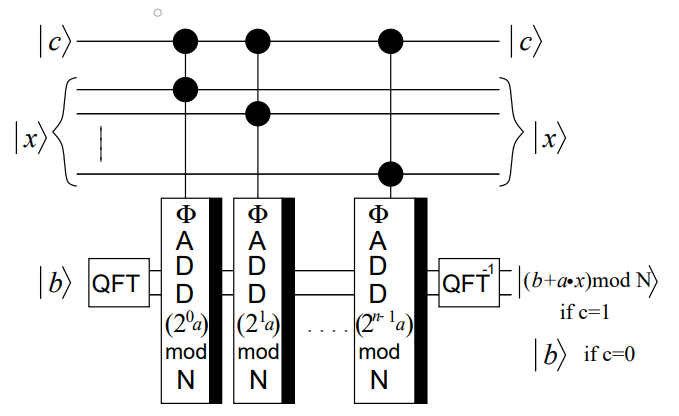
\includegraphics[scale = 0.6]{cmult.png}
  \caption{Kontrollierte Multiplikation nach Beauregard~\cite{beauregard2003circuit}}
  \label{fig:cmult}
\end{figure}


\bigskip

Der Code, der einen Quantenschaltkreis als Gatter gemäß dem Konzept in Abbildung~\ref{fig:cmult} generiert, 
ist in der Funktion \mintinline{python}{cmult_gate}~\ref{code:ModularMultiplication} definiert.

Die Funktion erwartet sowohl \(a\) als auch \(N\) als Parameter, 
jeweils in der Form einer Liste, welche die Zahl in Binärdarstellung beschreibt.
Dabei repräsentiert der erste Index beider Listen das Least-Significant-Bit.
Damit die unterliegenden modularen Addition Gatter für die korrekte Anzahl an Qubits gebildet werden, 
müssen die Listen jeweils die Länge n + 1 haben, wenn \(N\) der Größenordnung \(2^n\) entspricht.
Das Most-Significant-Bit sollte in beiden Listen dementsprechend den Wert \(0\) haben.
Des Weiteren erwartet die Funktion den Parameter \mintinline{python}{x_bits_amount}, der angibt, 
wie viele Qubits das Quantenregister \(\ket{x}_n\) umfasst 
und somit \(n\) entspricht. 

Um die Position der Qubits zu beschreiben, 
definiert die Funktion vier Wertebereiche.
\mintinline{python}{c_qbit} liegt an der ersten Stelle des kontrollierten Multiplikation Gatters und 
ist für das Kontrollqubit \(\ket{c}_1\) vorhergesehen.
Die darauffolgenden Qubits umfassen das \(\ket{x}_n\) Quantenregister und bestehen aus insgesamt \(n\) Qubits, 
deren Position in \mintinline{python}{c_qbit} definiert ist.
Die Position des \(\ket{b}_{n+1}\) Quantenregisters wird in \mintinline{python}{b_qbits} beschrieben.
Aufgrund der unterliegenden Gatter umfasst das \(\ket{b}_{n+1}\) Quantenregister ein zusätzliches Qubit, 
welches als Borrow-Bit dient.
Die Position des letzten Qubit \(\ket{0}_1\), 
wird mit \mintinline{python}{cond_qbit} definiert.
Dieses Qubit dient als Bedingungs-Qubit für die unterliegenden modularen Addition Gatter.

Im Code~\ref{code:ModularMultiplication} wird in Zeile 9. die Quanten-Fourier-Transformation auf 
das \(\ket{b}_{n+1}\) Quantenregister angewandt.
In Zeile 10 bis 13 folgen die Gatter zur modularen Addition.
Da \((b + a \cdot x) \bmod N\) äquivalent ist zu \((b + (a \cdot x)\bmod N) \bmod N\)~\cite{koepf_modular_2021}, 
wird einem Gatter der modularen Addition nicht der Parameter \(2^i\cdot a\) übergeben, 
sondern \({(2^i\cdot a)\bmod N}\).
Andernfalls wäre es notwendig, 
zusätzliche Qubits zu verwenden, um \(2^i\cdot a\) zu speichern.

Wie man in Zeile 13. sieht, teilen sich alle modularen Additions Gatter das selbe Bedingungs-Qubit \(\ket{0}_1\), 
welches sich auf der Position von \mintinline{python}{cond_qbit} befindet.
Genau aus diesem Grund, wird bei dem Gatter zur modularen Addition das Bedingungs-Qubit zurückgesetzt.

Abschließend wird noch die inverse Quanten-Fourier-Transformation auf das \(\ket{b}_{n+1}\) Quantenregister anwendet und 
der Quantenschaltkreis in ein Quantengatter umgeformt.

\begin{listing}[H]

\begin{minted}[linenos, fontsize=\customsize]{python}
def cmult_gate(x_bits_amount: int, a_bin: list[int],
                                   N_bin: list[int]) -> qiskit.circuit.gate:  
  a_dez = binToDez(a_bin)
  N_dez = binToDez(N_bin)
  c_qbit = [0]
  x_qbits =  list(range(1, x_bits_amount + 1))
  b_qbits = list(range(1+x_bits_amount, 1 + x_bits_amount + len(a_bin)))
  cond_qbit = [1 + x_bits_amount + len(a_bin)]
  cmult_gate = qiskit.QuantumCircuit(1 + x_bits_amount + len(a_bin) + 1)
  cmult_gate.append(QFT_Gate(len(b_qbits),inverse = False, MSB_first = False), b_qbits)
  for i in range(0, len(x_qbits)):
      a_i = ((2**(i)) *  a_dez) % N_dez
      a_i_bin = dezToBin(a_i, len(a_bin))
      cmult_gate.append(modular_adder_gate(a_i_bin, N_bin),
                        c_qbit+[x_qbits[i]]+b_qbits+cond_qbit)
  cmult_gate.append(QFT_Gate(len(b_qbits),inverse = True, MSB_first = False), b_qbits)
  cmult_gate = cmult_gate.to_gate()
  cmult_gate.name = "cmult " + str(a_dez) + " Mod " + str(N_dez)
  return cmult_gate
  \end{minted}
  \caption{Kontrollierte Multiplikation in Qiskit}
  \label{code:ModularMultiplication}
\end{listing}

In Qiskit wird der durch den Code gebildete Quantenschaltkreis wie in Abbildung~\ref{fig:cmult_qiskit} dargestellt.
Die Abbildung repräsentiert den Quantenschaltkreis für \(a = 11;~N = 15\).

Die Visualisierung der Kontroll-Abzweigungen ist anders als in den vorherigen Abbildungen dargestellt.
Dies liegt daran, dass die Kontrollqubits bereits in den unterliegenden Gattern, 
also der modularen Addition, 
definiert wurden.
Es ist möglich, die Kontrollqubits bei der Definition der modularen Adder Gatter auszulassen und 
stattdessen erst bei der Anwendung im kontrollierten Multiplikation Gatter anzuwenden, 
indem die Qiskit Funktion \mintinline{python}{control} verwendet wird.
Dadurch wird der Kontrolleffekt auf das gesamte Gatter zur modularen Addition angewendet, 
wodurch ein ineffizienterer Quantenschaltkreis entsteht, 
wie bereits im Abschnitt~\ref{sub:modulareAddition} zur modularen Addition erwähnt.

Es ist zu beachten, dass die Gatter zur modularen Addition in Abbildung~\ref{fig:cmult_qiskit} zwar über 
alle Qubits des \(\ket{x}_n\) Registers verlaufen, 
jedoch ausschließlich durch das Qubit kontrolliert werden, 
das im modularen Additions-Gatter den Index 1 trägt.

\begin{figure} [H]
  \centering
  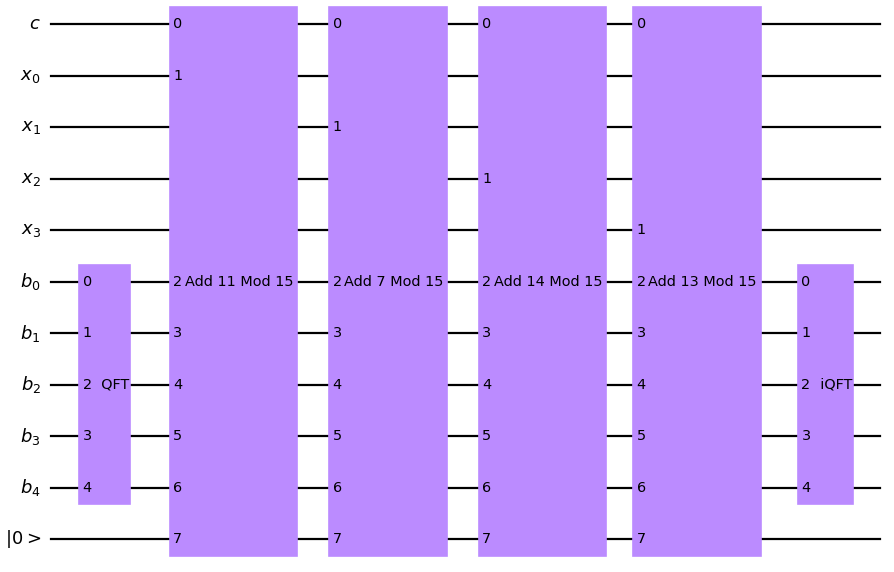
\includegraphics[scale = 0.5]{cmult_qiskit.PNG}
  \caption{Schaltkreis der kontrollierten Multiplikation in Qiskit}
  \label{fig:cmult_qiskit}
\end{figure}

Insgesamt wirkt das Gatter auf \(2n+3\) Qubits.
Diese setzen sich aus dem Kontrollqubit \(\ket{c}_1\), den \(n\) Qubits von \(\ket{x}_n\), 
den \(n+1\) Qubits von \(\ket{b}_{n+1}\) und dem einzelnen Bedingungs-Qubit \(\ket{0}_1\)zusammen.

Um der Inversen des kontrollierten Multiplikation Gatters eine eindeutige Benennung zu geben, 
wird dafür eine zusätzliche Funktion \mintinline{python}{inv_cmult_gate} definiert.
\begin{listing}[H]
\begin{minted}[linenos,fontsize=\customsize]{python}  
def inv_cmult_gate(x_bits_amount: int, a_bin: list[int],
                                       N_bin: list[int]) -> qiskit.circuit.gate:  
  inv_cmult_gate = cmult_gate(x_bits_amount,a_bin,N_bin).inverse()
  inv_cmult_gate.name = "inv cmult " + str(binToDez(a_bin)) 
                      + " Mod " + str(binToDez(N_bin))
  return inv_cmult_gate
  \end{minted}
  \caption{Inverse kontrollierte Multiplikation in Qiskit}
  \label{code:InverseModularMultiplication}
\end{listing}

\subsubsection{Vollständige Transformation}

Das letzte zu konstruierende Gatter wird als \(U_a\)-Gatter bezeichnet, 
weil es die benötigte Transformation realisiert: 
\[U^{\tensor n}\ket{y}_n = \ket{ay \bmod N}_n\] 
Das \(U_a\)-Gatter dient zur Realisierung der Quantum"=Phase"=Estimation im Shor"=Algorithmus, 
wie in Abbildung~\ref{fig:shor_n_qubit} dargestellt.

Dafür nimmt das \(U_a\)-Gatter vier Quantenregister entgegen und 
führt die folgende Transformation durch: 
\[\ket{c}_1\ket{x}_{n}\ket{0}_{n+1}\ket{0}_1
\longrightarrow
\ket{c}_1\ket{(a x) \bmod N}_{n}\ket{0}_{n+1}\ket{0}_1
\]

Um ein \(U_a\)-Gatter zu realisieren, benötigt man im Grunde kontrollierte Swap-Gatter und 
lediglich zwei Gatter zur kontrollierten Multiplikation. 
 
Im Folgenden wird die Auswirkung der einzelnen Bestandteile des \(U_a\)-Gatter erklärt.
Dabei werden von den vier Quantenregistern nur die beiden 
Quantenregister \(\ket{x}_{n}\ket{0}_{n+1}\) beachtet.
Das Qubit \(\ket{c}_1\) wie auch \(\ket{0}_1\) verzeichnet während der Transformation keine Veränderung, 
welche für das Verständnis des \(U_a\)-Gatter relevant ist.

Der Ablauf des \(U_a\)-Gatter lautet wie folgt:
Als erstes wird ein Gatter zur kontrollierten Multiplikation mit \(a\) angewendet. 
Dieses Gatter führt, 
ausgehend vom initialen Zustand der beiden Quantenregister, 
die folgende Transformation durch~\cite{beauregard2003circuit}:
\[
  \ket{x}_{n}\ket{0}_{n+1}
  \longrightarrow
  \ket{x}_{n}\ket{(ax)\bmod N}_{n+1}
  \]

Darauf folgen kontrollierte Swap-Gatter, die beide Zustände vertauschen:
\[
  \ket{x}_{n}\ket{(ax)\bmod N}_{n+1}
\longrightarrow
\ket{(ax)\bmod N}_{n}\ket{x}_{n+1}
\]
Dabei ist zu beachten, 
dass das zweite Quantenregister aus \(n+1\) Qubits besteht und
somit ein Qubit mehr besitzt als das erste Quantenregister.
Da das Most-Significant-Bit des zweiten Quantenregisters zu diesem Zeitpunkt garantiert im Zustand \(\ket{0}\) ist, 
kann es vernachlässigt werden und wird daher keiner Swap-Operation unterzogen.

Nach dem Swap wird ein inverses Gatter zur kontrollierten Multiplikation angewendet.
Dabei wird dem inversen Gatter zur kontrollierten Multiplikation statt dem Element \(a\) 
das multiplikative Inverse von \(a\) in den Einheiten des Restklassenrings \(N\) übergeben, 
also \(a^{-1} \bmod N\).
Als Folge davon verändert sich der Zustand der Quantenregister folgendermaßen:  
\[\ket{(ax)\bmod N}_{n}\ket{x}_{n+1}
\longrightarrow
\ket{(ax)\bmod N}_{n}\ket{(x-a^{-1}ax)\bmod N}_{n+1}
\] 
Der Ausdruck \((a^{-1}a)\bmod N\) entspricht dem neutralen Element 1, 
weswegen der Zustand der Quantenregister wie folgt vereinfacht werden kann:  
\[
\ket{(ax)\bmod N}_{n}\ket{(x-a^{-1}ax)\bmod N}_{n+1}
=
\ket{(ax)\bmod N}_{n}\ket{0}_{n+1}
\] 

Beachtet man den Eingangs- und Ausgangszustand der beiden Quantenregister, 
so bewirkt das \(U\)-Gatter eine Transformation von:
 \[\ket{x}_{n}\ket{0}_{n+1} 
 \longrightarrow 
 \ket{(ax)\bmod N}_{n}\ket{0}_{n+1}\]

Das Konzept des Aufbaus des Quantenschaltkreises ist in Abbildung~\ref{fig:u_gatter} dargestellt.
\begin{figure} [H]
  \centering
  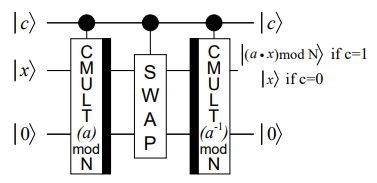
\includegraphics[scale = 0.8]{u_gatter.png}
  \caption{\(U_a\)-Gatter~\cite{beauregard2003circuit}}
  \label{fig:u_gatter}
\end{figure}

Die Funktion \mintinline{python}{U_gate}~\ref{code:UGatter} enthält den Code zur Generierung eines \(U_a\)-Gatters.
Dazu nimmt die Funktion dieselben Parameter wie die Funktion \mintinline{python}{cmult_gate} entgegen, 
nämlich  \mintinline{python}{a_bin} und \mintinline{python}{N_bin}, welche jeweils \(a\) und \(N\) in binärer Form im Listenformat beschreiben,  
sowie \mintinline{python}{x_bits_amount}, das im Grunde \(n\) repräsentiert.

Im Code~\ref{code:UGatter} werden insgesamt fünf Wertebereiche definiert.
Das Kontrollqubit \(\ket{c}_1\) befindet sich auf der Position \mintinline{python}{c_qbit},
gefolgt von \mintinline{python}{x_qbits} für das \(\ket{x}_{n}\) Quantenregister und  
\mintinline{python}{b_qbits} für die Qubits von \(\ket{0}_{n+1}\).
Das Bedingungs-Qubit wird auf der letzten Position des Gatters platziert und  
ist in \mintinline{python}{cond_qbit} festgelegt.
Des Weiteren wird \mintinline{python}{full_range} verwendet,
um alle vier vorherigen Quantenregister zu umfassen.

Wie in Zeile 7. des Codes ersichtlich, wird zuerst ein Gatter zur kontrollierten Multiplikation eingesetzt.
Dafür werden der Funktion \mintinline{python}{cmult_gate} die Parameter \mintinline{python}{a_bin}, \mintinline{python}{N_bin} und \mintinline{python}{x_bits_amount} übergeben.
Das Gatter zur kontrollierten Multiplikation wird auf den gesamten Bereich \mintinline{python}{full_range} angewendet, 
somit umfasst das \(U_a\)-Gatter \(2n+3\) Qubits.
In Zeile 9 und 10 werden die kontrollierten Swap-Gatter eingesetzt.
Wie man in Zeile 10. erkennt, bezieht sich die Wirkung eines Swap-Gatters auf denselben Index von \mintinline{python}{x_qbits} und \mintinline{python}{b_qbits}.
Somit werden die Qubits beider Quantenregister vertauscht, die die gleiche Wertigkeit haben.
In Zeile 11. wird \(a^{-1}\bmod N\) mittels des erweiterten euklidischen Algorithmus berechnet.
Anschließend wird das berechnete \(a^{-1}\bmod N\) als Parameter an ein inverses kontrolliertes Multiplikation Gatter übergeben.
Abschließend wird der Quantenschaltkreis zu einem Gatter umgeformt und passend benannt.

\begin{listing}[H]
\begin{minted}[linenos,fontsize=\footnotesize]{python}  
def U_gate(x_bits_amount: int, a_bin: list[int],
                               N_bin: list[int]) -> qiskit.circuit.gate:  
  c_qbit = [0]
  x_qbits =  list(range(1, x_bits_amount + 1))
  b_qbits = list(range(1+x_bits_amount, 1 + x_bits_amount + len(a_bin)))
  cond_qbit = [1 + x_bits_amount + len(a_bin)]
  full_range = c_qbit + x_qbits + b_qbits + cond_qbit
  U_a_gate = qiskit.QuantumCircuit(len(full_range))
  U_a_gate.append(cmult_gate(x_bits_amount,a_bin ,N_bin), full_range)
  for i in (range(x_bits_amount)):
      U_a_gate.cswap(c_qbit,x_qbits[i],b_qbits[i])
  a_inv_bin = dezToBin(\gcd(binToDez(a_bin),binToDez(N_bin)),len(a_bin))
  U_a_gate.append(inv_cmult_gate(x_bits_amount,a_inv_bin ,N_bin), full_range)
  U_a_gate = U_a_gate.to_gate()
  U_a_gate.name = "  U_" + str(binToDez(a_bin))
  return U_a_gate
  \end{minted}
  \caption{\(U\)-Gatter in Qiskit}
  \label{code:UGatter}
\end{listing}

Der Quantenschaltkreis, der durch den Code~\ref{code:UGatter} gebildet wird, 
wird in Qiskit wie in Abbildung~\ref{fig:u_gatter_qiskit} dargestellt. 
Die Abbildung zeigt ein Beispiel für \(a=7\) und \(N=15\).

\begin{figure}[H]
  \centering
  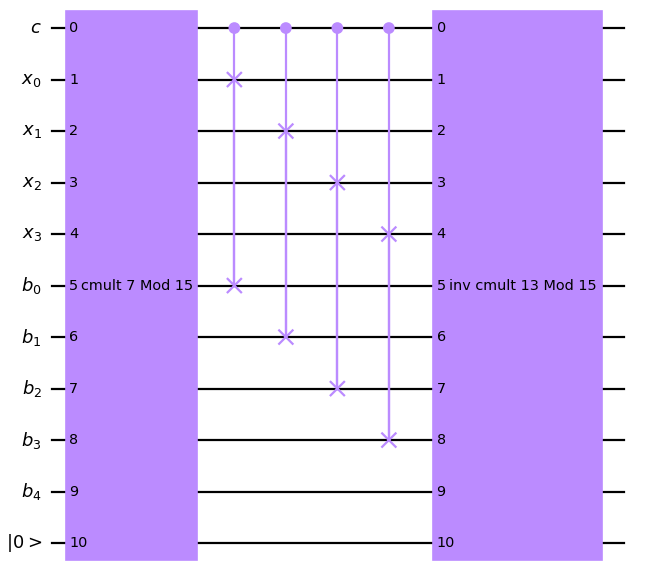
\includegraphics[scale = 0.5]{u_gatter_qiskit.PNG}
  \caption{\(U_a\)-Gatter in Qiskit}
  \label{fig:u_gatter_qiskit}
\end{figure}

\subsubsection{Quantum-Phase-Estimation für Shor} \label{section:imp_QPE_Shor}
Der letzte Schritt zur Komplettierung des Quantenschaltkreises für den Quantenalgorithmus, 
der in der Lage ist, 
die Periode zu bestimmen, besteht darin, 
die Quantum-Phase-Estimation wie in Abbildung~\ref{fig:shor_n_qubit} unter Verwendung des \(U_a\)-Gatters zu bilden.

In Abbildung~\ref{fig:shor_n_qubit} werden unter anderem \({U_a}^{2^x}\)-Gatter eingesetzt.
Diese können realisiert werden, 
indem ein \({U_a}\)-Gatter insgesamt \(2^x\) mal hintereinander geschaltet wird oder 
indem anstelle von \(a\) der Parameter \(a^{2^x}\) an ein einzelnes \(U_a\)-Gatter übergeben wird.
Die zweite Variante ist möglich wegen~\cite{beauregard2003circuit}:
\[(a^nx)\bmod N = \underbrace{(a\dotsc(((a(ax)\bmod N)\bmod N)\dotsc)\bmod N)}_{\text{\(n\) mal}}\]

Bei der Wahl zwischen den beiden Varianten liegt das entscheidende Kriterium bei der Ressourceneffizienz. 
Die zweite Variante schneidet dabei deutlich besser ab, 
da sie lediglich \(x\) viele \(U_a\)-Gatter benötigt, 
wenn \(x\) viele Kontrollqubits verwendet werden, 
im Gegensatz zur ersten Variante, die \(2^x-1\) viele \(U_a\)-Gatter erfordert.

Ein weiterer wichtiger Aspekt für den Aufbau der Quantenschaltung betrifft die Anzahl der benötigten Kontrollqubits.
Beauregard erklärt in seinem Paper~\cite{beauregard2003circuit} nicht, 
warum er eine Konstruktion mit insgesamt \(2n\) Kontrollqubits beziehungsweise \({U_a}^{2^x}\)-Gatter wählt.
Es gibt Quellen, die mehr als \(2n\)  Kontrollqubits verwendeten~\cite[229]{nielsen_chuang_2010}.
Nach dem Paper von Peter Shor~\cite{Shor_1997} sind jedoch \(2n\) Kontrollqubits ausreichend,
wie auch im Abschnitt~\ref{Funktionsweise:klassisch} erläutert wird.
Deswegen verwendet die hier implementierte Variante \(2n\) Kontrollqubits.

\bigskip

Der Code für einen Quantenschaltkreis wie in Abbildung~\ref{fig:shor_n_qubit} ist in der Funktion 
\mintinline{python}{Shor}~\ref{code:Periodenbestimmung} enthalten.

Die Funktion erwartet die beiden Zahlen \(a\) und \(N\) als Parameter.
Des Weiteren kann der Funktion über den Parameter \mintinline{python}{number_shots} mitgeteilt werden, 
mit wie vielen Durchläufen der Quantenalgorithmus ausgeführt werden soll.
Jeder Durchlauf gewährt ein weiteres Messergebnis.
Der Parameter \mintinline{python}{backend} ist dazu da, 
um festzulegen, auf welchem System der Quantenalgorithmus ausgeführt werden soll.
Standardmäßig wird der Simulator von Qiskit genutzt. 
Falls Zugang zu einem Quantensystem von IBM besteht, 
würde man stattdessen die Bezeichnung der entsprechenden Quantum-Backend verwenden.

Die Funktion \mintinline{python}{Shor} definiert die beiden Wertebereiche \mintinline{python}{c_qbits} und 
\mintinline{python}{ev_qbits}, um die Positionen der beiden Quantenregister zu beschreiben.
Der Wertebereich \mintinline{python}{c_qbits} enthält die insgesamt \(2n\) Positionen der Kontrollqubits.
Der Eigenvektor wird in den Qubits gespeichert, 
deren Position in \mintinline{python}{ev_qbits} definiert ist.

Der Quantenschaltkreis wird in der 5. Zeile definiert und umfasst \(4n+2\) Qubits und 
\(2n\) klassische Bits, welche zum Messen verwendet werden.
In Zeilen 6 und 7 wird ein Hadamard-Gatter auf jedes Kontrollqubit angewendet.
In den der 8. Zeile wird der Eigenvektor gebildet. 
Da der Eigenvektor dem Zustand \(\ket{1}\) entspricht,
genügt es, wenn das Least-Significant-Qubit mit einem X-Gatter versehen wird.
In den Zeilen 9 und 10 werden die zugehörigen \({U_a}^{2^x}\)-Gatter mit dem passenden \(x\) auf das Register mit dem Eigenvektor angewendet.
Die Funktion \mintinline{python}{mod_exp} berechnet \((a^{2^x})\bmod N\).
In der 11. Zeile werden die Kontrollqubits mit der inverse Quanten-Fourier-Transformation in die Standardbasis transformiert.  
Da die Funktion \mintinline{python}{Shor} Messungen durchführen soll, 
wird in der 12. Zeile definiert, dass die Kontrollqubits gemessen werden.
In dem Fall entspricht dies den Qubits auf den Positionen \mintinline{python}{c_qbits}.
Anschließend werden in den Zeilen 13 und 14 \mintinline{python}{number_shots} viele Messungen durchgeführt und 
das Ergebnis wird als Rückgabewert der Funktion zurückgegeben.

Wie bei der Definition des Quantenschaltkreises in Zeile 5. erkennbar, 
benötigt der Quantenschaltkreis \(4n+2\) Qubits anstatt \(2n+3\).
Die Reduktion der benötigten Qubits wird in der Sektion~\ref{Optimierung} thematisiert. 

\begin{listing}[H]
\begin{minted}[linenos,fontsize=\customsizetwo]{python}  
def Shor(a: int, N: int,number_shots: int = 1000, backend: str = "aer_simulator"):
  n = N.bit_length()
  c_qbits = range(2*n)
  ev_qbits = list(range(len(c_qbits),4*n+2))
  qc = qiskit.QuantumCircuit(4*n+2,len(c_qbits)) 
  for c_bit in c_qbits:
    qc.h(c_bit)
  qc.x(ev_qbits[0])
  for c_bit in c_qbits:
    qc.append(U_gate(n,dezToBin(mod_exp(a,2**c_bit,N),n+1),dezToBin(N,n+1)),
              [c_bit]+ev_qbits)
  qc.append(QFT_Gate(len(c_qbits),inverse = True, MSB_first = False,swaps = True),
            c_qbits)
  qc.measure(c_qbits,c_qbits)
  simulator = qiskit.Aer.get_backend(backend)
  sim_result = qiskit.execute(qc, backend=simulator, shots=number_shots).result()
  return sim_result.get_counts(qc)
  \end{minted}
  \caption{Periodenbestimmung in Qiskit}
  \label{code:Periodenbestimmung}
\end{listing}

In Abbildung~\ref{fig:shor_qiskit} ist der Quantenschaltkreis zu sehen, 
der durch die Funktion \mintinline{python}{Shor} für \(a=7;~N=15\) generiert wird.
Bei \(N=15\) tritt der Effekt auf, dass für \(x>1\) die Rechnung \((a^{2^x})\bmod N = 1\) ergibt, 
weshalb auch die \({U_a}^{2^x}\)-Gatter zu \(U_1\) werden.

\begin{figure}[H]
  \centering
  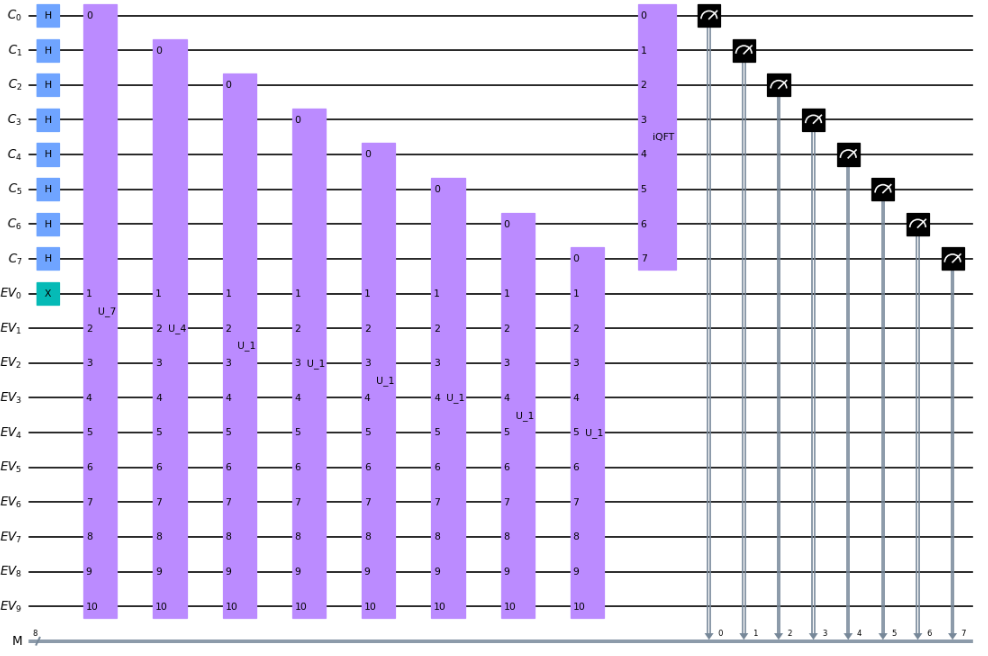
\includegraphics[scale = 0.6]{shor_qiskit.PNG}
  \caption{Quantenalgorithmus von Shor in Qiskit}
  \label{fig:shor_qiskit}
\end{figure}

\subsection{Faktorisierungsalgorithmus} \label{sec:Faktorisierungsalgorithmus}
Der Faktorisierungsalgorithmus kombiniert die Quantum-Phase-Estimation zur Periodenberechnung mit  
der klassischen Nachberechnung. 
Der Hauptfokus der Implementierung liegt darauf, 
die Schwächen der Messergebnisse der Quantum-Phase-Estimation mithilfe klassischer Methoden zu kompensieren.

Es ist zu erwarten, 
dass die Ausführung von Quantenberechnungen auch mit zukünftig fortschrittlichen Quantencomputern kostenintensiv sein wird~\cite{Shor_1997}.
Daher wäre es ineffizient, 
die Quantum-Phase-Estimation so oft zu wiederholen, 
bis ein Ergebnis erzielt wird, dass die Periode direkt offenbart.
Stattdessen ist es ressourcensparender, 
ein erhaltenes Messergebnis, 
unter Berücksichtigung der in Abschnitt~\ref{Funktionsweise:klassisch} erklärten drei möglichen Szenarien,
mit klassischen Methoden aufzubereiten. 
Als Resultat können so weitere Durchläufe der Quantum-Phase-Estimation eingespart und 
durch klassische Rechenleistung ersetzt werden.

\bigskip

Die Grafik~\ref{fig:shor_measure} repräsentiert insgesamt 512 Messungen für \(a=19;~N=119\), 
mit einer Genauigkeit \(k\) von \(2\ld(119) \approx 14 \). 
Ihr Zweck ist es, die Besonderheiten, 
welche bei Messergebnissen auftreten können, hervorzuheben.
Zur Verdeutlichung sind die Messergebnisse in Abbildung~\ref{fig:shor_measure} in vier Kategorien eingeteilt.
Die Kriterien für die Einteilung in diese Kategorien basieren darauf, 
ob nach der Division durch \(2^k\) und 
der Anwendung des Kettenbruch-Algorithmus mit einem Nenner kleiner als \(N\), 
die Periode erfolgreich extrahiert werden kann.

Die grünen Ergebnisse offenbaren direkt die gesuchte Periode von \(p = 24\).
Ein Faktorisierungsalgorithmus, welcher so lange die Quantum-Phase-Estimation wiederholt, 
bis ein Messergebnis die ungekürzte Periode enthält, 
wird ausschließlich bei den grünen Ergebnissen erfolgreich sein.

Anhand der gelben Ergebnisse kann die gesuchte Periode nicht direkt extrahiert werden.
Dabei ist der Fall eingetreten, dass der Zähler und Nenner des Bruches einen gemeinsamen Teiler hatten, 
weshalb der Bruch gekürzt wurde.
Gegebenenfalls kann die Periode mit klassisch ausführbaren Methoden rekonstruiert werden.

Die hellroten Ergebnisse sind zu weit vom Peak entfernt,
weswegen diese die gesuchte Periode weder vollständig noch gekürzt enthalten.
Womöglich kann die Periode aus diesem Messergebnis ermittelt werden, 
wenn die benachbarten Zustände überprüft werden.

Die beiden dunkelroten Zustände sind die beiden Zustände der finalen Superposition
\(\ket{2^k \cdot \frac{0}{p}}_k\) und \(\ket{2^k \cdot \frac{p/2}{p}}_k\).
Der Zustand \(\ket{2^k \cdot \frac{0}{p}}_k\) existiert für jede Zahl und erlaubt keine 
Rückschlüsse auf die Periode.
Der andere Zustand \(\ket{2^k \cdot \frac{p/2}{p}}_k\) existiert ausschließlich, wenn \(p\) gerade ist.
Auch dieser Zustand gewährt keine hilfreichen Rückschlüsse auf die Phase, 
da \(\frac{p/2}{p}\) immer zu \(\frac{1}{2}\) gekürzt wird.
Eine notwendige Bedingung, um die Faktoren aus \(p\) herleiten zu können, 
ist, dass \(p\) gerade ist~\cite*{Shor_1997}, 
dies wird zwar durch die Messung von \(\ket{2^k \cdot \frac{p/2}{p}}_k\) bestätigt, 
jedoch kann aus dieser Information keine hilfreiche Konsequenz gezogen werden.

\begin{figure}[H]
  \centering
  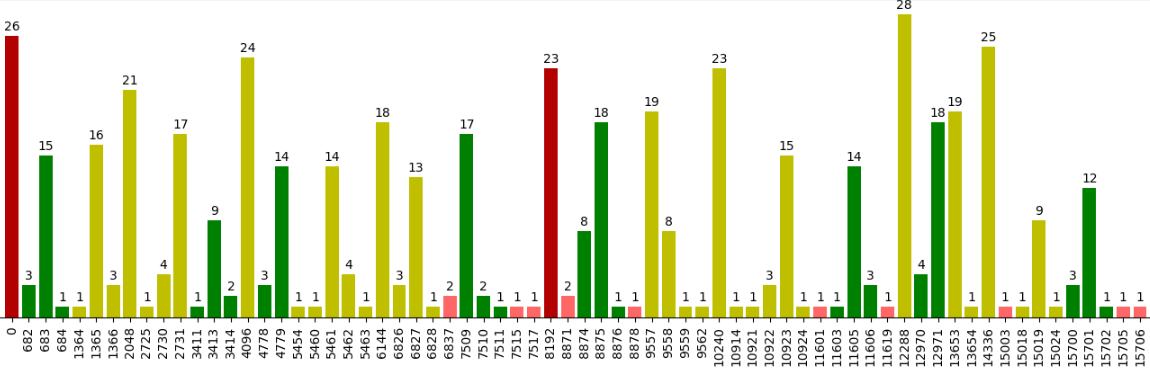
\includegraphics[scale = 0.5]{Messung_beispiel.PNG}
  \caption{Beispiel Messung a=19, N=119, k=14}
  \label{fig:shor_measure}
\end{figure}


\bigskip

Abbildung~\ref{fig:Flussdiagramm} gibt einen Überblick über den Ablauf des Algorithmus 
von der Berechnung der Periode bis zur Bestimmung der Primfaktoren.

Am Anfang des Algorithmus wird zufällig ein \(a\) definiert, 
welches größer als 1, aber kleiner als \(N\) ist.

Für den ungewöhnlichen Fall, dass \(a\) einen gemeinsamen, nicht-trivialen Teiler mit \(N\) hat, 
ist dieser einer der gesuchten Faktoren von \(N\), 
weswegen der Algorithmus terminiert.
Die Überprüfung, ob \(a\) und \(N\) einen Faktor teilen, 
kann mit Euklids Algorithmus mit maximal polynomialen Aufwand berechnet werden~\cite[301]{homeister2023quantum215}. 
Euklids Algorithmus ist in der Lage, den größten gemeinsamen Teiler (\(\gcd\)) zu berechnen.

Anschließend wird zu dem gewählten \(a\) ein Set erstellt.
Dieses Set wird dafür genutzt, um die Brüche zu speichern, 
bei denen die Periode nicht im Nenner steht. 
Die gespeicherten Brüche enthalten in ihrem Nenner womöglich Teiler der gesuchten Periode, 
welche bei weiteren Berechnungen dabei helfen könnten, die Periode zu finden.

Darauf folgt der einzige quantenalgorithmische Bestandteil der Berechnung, 
welcher auf einem Quantencomputer ausgeführt wird.
Konkret geht es um die Ausführung der für die Periodenbestimmung angepassten Quantum-Phase-Estimation. 
Für ein ressourceneffizienteres Vorgehen wird nur ein Durchlauf der Quantum-Phase-Estimation angestoßen.
Anhand des einzelnen Messergebnisses wird die Berechnung fortgesetzt.

Die nächsten Berechnungen werden wieder auf einem klassischen Rechnersystem ausgeführt.
Bei der Berechnung wird das Messergebnis aus dem Binärsystem ins Dezimalsystem umgewandelt
und durch die entsprechende 2er-Potenz geteilt.
Nachdem das Ergebnis ermittelt wurde, 
wird der Kettenbruch-Algorithmus angewendet. 
Dieser Algorithmus findet aufgrund der festgelegten Limitation den nächstgelegenen Bruch mit einem Nenner kleiner als \(N\).
Dieser Schritt ist ebenfalls mit einem maximal polynomialen Aufwand durchführbar~\autocite[230]{nielsen_chuang_2010}.

Im nächsten Schritt wird überprüft, ob der Nenner des Bruches der Periode entspricht.
Im ersten Durchlauf wird dies nur der Fall sein, 
wenn die Messung einen der Zustände ergeben hat, 
die wie in Abbildung~\ref{fig:shor_measure} zu der farblich grünen Kategorie gehört.
Sollte es nicht möglich sein, die Periode direkt zu extrahieren, 
wird anhand des Messergebnisses eine Nachberechnung angestoßen.

Der erste Schritt in der Nachberechnung besteht darin, 
zu überprüfen, ob ein Vielfaches des Nenners die Periode darstellt.
Dabei ist zu beachten, bis zu welchem Vielfachen diese Überprüfung durchgeführt wird. 
Ein sinnvoller Ansatz wäre, eine Obergrenze festzulegen, die logarithmisch mit \(n\) wächst.
Andernfalls könnte es bei sehr großen Werten für \(N\) passieren, 
dass zu viele klassische Berechnungen anfallen würden, die in keinem vertretbaren Zeitaufwand durchführbar wären.
In der Implementierung werden die Vielfachen mit einer Multiplikation von \(2\) bis \(2^{\ld(n)}\) getestet.

Sollte die Periode keines der getesteten Vielfachen des Nenners darstellen, 
wird das kleinste gemeinsame Vielfache (\(\lcm\)) des aktuellen Nenners mit den einzelnen Nennern aus dem Set gebildet.
Falls die beiden zugehörigen Zähler keinen Faktor teilen, 
kann mit einer Wahrscheinlichkeit größer als \(0.25\) die Periode aus dem \(\lcm\) berechnet werden~\cite[231]{nielsen_chuang_2010}.

Die beiden vorherigen Methoden können zum Erfolg führen, 
falls ein Messergebnis, wie in Abbildung~\ref{fig:shor_measure}, 
zur gelben Kategorie gehört. 

Wenn beide vorherigen Methoden fehlschlagen, 
wird angenommen, dass das Messergebnis einer der beiden roten Kategorien angehört.
In diesem Fall wird überprüft, ob einer der Nachbarn die Periode enthält.
Damit der Aufwand nicht den Rahmen der Laufzeit sprengt, 
werden genau wie bei der Überprüfung der Vielfachen
nur eine begrenzte Anzahl an Nachbarn getestet.
Genau wie bei der Überprüfung der Vielfachen werden in der Implementierung alle Nachbarn durch 
die Addition beziehungsweise Subtraktion des Messwertes von \(1\) bis \(2^{\ld(n)}\) getestet.

Falls einer der Nachbarn die Periode enthält, 
handelt es sich bei dem Zustand des Nachbarn um einen, 
welcher der grünen Kategorie angehört, 
wie beispielsweise in Abbildung~\ref{fig:shor_measure} der Zustand \(\ket{8878}_{14}\).

Es ist möglich, 
dass die Zustände der Nachbarn des Messergebnisses der gelben Kategorie angehören.
In diesem Fall ist eine direkte Extraktion nicht möglich, 
weswegen auch die Vielfachen und das \(\lcm\) von einem benachbarten Zustand geprüft wird.
In Abbildung~\ref{fig:shor_measure} repräsentiert der Zustand \(\ket{6837}_{14}\) dieses Szenario.

Sollte trotz der Nachberechnung keine Periode extrahiert werden können, 
wird der Bruch des Messergebnisses im Set gespeichert.
Anschließend wird ein neuer Durchlauf der Quantum-Phase-Estimation 
mit demselben \(a\) durchgeführt.

Im Falle, dass die Periode direkt extrahiert werden konnte oder 
durch die Nachberechnung bestimmt wurde, wird überprüft, 
ob die Periode einer geraden Zahl entspricht und die folgende Bedingung erfüllt:
\[a^{\frac{p}{2}} = -1 \bmod N\]
Wenn beide Kriterien zutreffen, 
kann mit der Periode und 
Euklids Algorithmus mindestens einer der beiden nicht-trivialen Faktoren von \(N\) berechnet werden~\cite{Shor_1997}:
\[\gcd(a^{\frac{p}{2}}-1, N), \gcd(a^{\frac{p}{2}}+1, N)\]
Anschließend terminiert der Algorithmus. 

Im Falle, dass nur ein Faktor gefunden wurde, kann der zweite berechnet werden, 
indem \(N\) durch den gefundenen Faktor dividiert wird.

Falls die Periode ungerade ist oder die zweite Bedingung nicht erfüllt ist, 
ist es nicht möglich, aus der gefundenen Periode die Faktoren zu berechnen~\cite{Shor_1997}.
In diesem Fall wird ein neues \(a\) gewählt und ein neues leeres Set definiert. 
Das alte Set beinhaltet Informationen zur Periode des vorherigen \(a\).
Anschließend wird mit dem neuen \(a\) die Quantum-Phase-Estimation ausgeführt und 
die Berechnung wiederholt.

Im Flussdiagramm und in der Beschreibung 
wird die Ausführung des Quantenalgorithmus praktisch als ein sequenzieller Abschnitt dargestellt, 
welcher erst durch einen gewissen Punkt in der klassischen Berechnung angestoßen wird.
Dies ist aber nur der Fall, bis das erste \(a\) bestimmt wird.
Da der Quantenalgorithmus und die klassischen Berechnungen auf zwei unterschiedlichen Systemen laufen~\cite{IBMQuantumServerless2023}, 
ist es möglich, parallel zur klassischen Nachberechnung, 
bereits einen weiteren Durchlauf der Quantenberechnung durchzuführen. 
Allerdings kann es bei diesem Vorgehen dazu kommen, 
dass die erste Messung bereits die korrekte Periode offenbart, 
weswegen eine parallele zweite Messung unnötige Quanten-Ressourcen beansprucht.

\begin{figure} 
  \centering
  % Use textheight minus 1 line for caption minus 1 line skip
  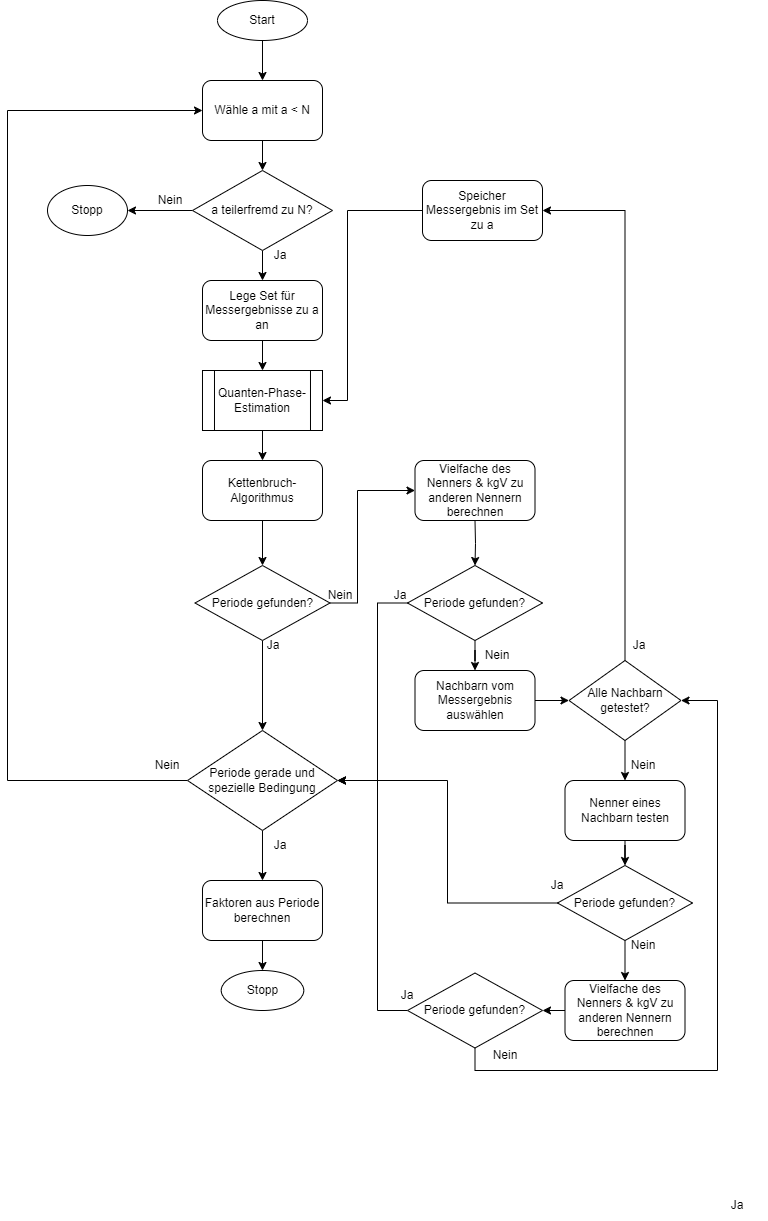
\includegraphics[height=\dimexpr\textheight-2\baselineskip]{FlussdiagramFaktorisierung.png}
  \caption{Flussdiagramm Faktorisierung}
  \label{fig:Flussdiagramm}
\end{figure}

\subsection{Optimierung} \label{Optimierung}
Die folgende Sektion thematisiert zwei mögliche Methoden, 
um den Ressourcenbedarf der Quantenbrechung zu reduzieren.
Beide Optimierungen kommen mit einer Abwägung, 
die gewisse Nachteile mit sich bringt,
wodurch im Gegenzug jedoch Ressourcen eingespart werden.
Somit handelt es sich bei den Optimierungen um Lösungen, 
die situationsbedingt besser sind.
Dabei sind die Eigenschaften und die Architektur des genutzten Quantencomputers die ausschlaggebenden Kriterien.

\subsubsection{Iterative Quantumten-Phase-Estimation}
In den vorherigen Kapiteln wurde die Quantum-Phase-Estimation in der Standardvariante, 
wie in Sektion~\ref{Quanten-Phase-Estimation} beschrieben, verwendet.
In der Standardvariante wird für jedes \(U^{2^x}\)-Gatter ein eigenes Kontrollqubit benötigt.
Dies bedeutet, wenn \(2n\) viele \(U^{2^x}\)-Gatter angewendet werden sollen, 
sind genau so viele Kontrollqubits nötig.

Ein zentraler Bestandteil der Quantum-Phase-Estimation ist die (inverse) Quanten-Fourier-Transformation. 
Wie im Abschnitt~\ref{Quanten-Fourier-Transformation} gezeigt, 
hängt die Wirkung dieser Transformation auf ein einzelnes Qubit von den Zuständen der anderen Qubits ab 
und zwar aufgrund von kontrollierten Phasenverschiebungen.

Bei der regulären Quanten-Fourier-Transformation kontrolliert ein bestimmtes Qubit zunächst die Phasen-Gatter auf die übrigen Qubits, 
bevor auf das kontrollierende Qubit selbst ein Hadamard-Gatter angewendet wird.
Das bedeutet, dass die kontrollierten Gatter der regulären Quanten-Fourier-Transformation abhängig sind von dem Eingangszustand.

Dies sieht bei der inversen Quanten-Fourier-Transformation anders aus.
Bei der inversen Quanten-Fourier-Transformation wird auf ein Qubit zuerst ein Hadamard-Gatter angewendet, 
erst danach kontrolliert es die Phasen-Gatter auf die anderen Qubits.
Dementsprechend sind bei der inversen Quanten-Fourier-Transformation die kontrollierten Gatter abhängig von dem Ausgangszustand.

Die Abhängigkeit zum Ausgangszustand ermöglicht es, 
die inverse Quanten-Fourier-Transformation aufzuteilen und die Bestandteile iterativ anzuwenden.
Dadurch wird der Ressourcenbedarf der Quantum-Phase-Estimation von \(2n\) Kontrollqubits auf ein einzelnes reduziert~\cite{Parker2000}.

In der Standardvariante der Quanten-Fourier-Transformation kontrollieren Qubits die Phasen-Gatter.
In der semi-klassischen beziehungsweise, iterativen Variante ist dies anders.
Diese Methode kam erstmals 1995 zum Einsatz und 
nutzt das klassische Signal einer Messung, 
um ein Quanten-Gatter zu kontrollieren~\cite{Griffiths_1996}.
Im Kern der Optimierung liegt der Trick darin, 
das Messergebnis des jeweiligen Qubits als Steuerungsbedingung für ein Phasen-Gatter zu verwenden.

Die Quantum-Phase-Estimation verwendet die inverse Quanten-Fourier-Transformation mit Swap-Gattern.
Da die identische Transformation benötigt wird, 
muss die iterative Variante das Verhalten der Swap-Gatter berücksichtigen.
Zur besseren Verständlichkeit ist die inverse Quanten-Fourier-Transformation mit Swap-Gattern in Abbildung~\ref{fig:iQFTswaps} dargestellt.
\begin{figure}[H]
  \centering
  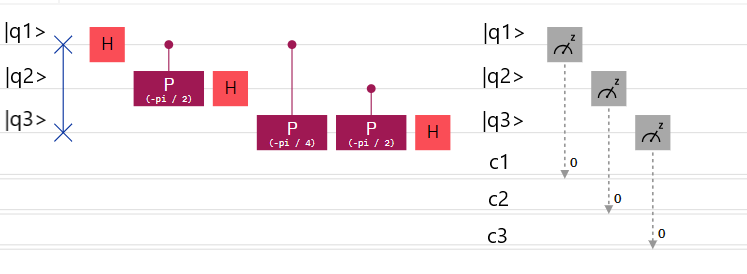
\includegraphics[scale = 0.6]{iqft_3qubit_swaps.PNG}
  \caption{3 Qubits inverse QFT mit Swaps}
  \label{fig:iQFTswaps}
\end{figure}
Wie in Abbildung~\ref{fig:iQFTswaps} dargestellt, 
wird das Eingangsqubit \(\ket{q3}_1\), welches das Most-significant-Bit enthält, 
mit \(\ket{q1}_1\) getauscht. 
Anschließend wird ein Hadamard-Gatter angewendet, 
wodurch das \(\ket{q3}_1\) Qubit in die Standardbasis transformiert wird. 
Erst danach kontrolliert das \(\ket{q3}_1\) Qubit zwei Phasen-Gatter.
Der Messwert wird in dem klassischen Bit \(c1\) gespeichert.
Das gleiche Verhalten kann, wie in Abbildung~\ref{fig:iterative_iQFT} gezeigt, nachgestellt werden, 
indem nach der Anwendung des Hadamard-Gatters auf das \(\ket{q3}_1\) Qubit 
der Messwert im klassischen Bit \(c1\) gespeichert wird.
Anschließend kontrolliert das klassische Bit \(c1\) die Phasen-Gatter.

Um nach der Messung dasselbe Kontrollqubit für \(\ket{q2}_1\) verwenden zu können, 
muss dieses in einen eindeutigen Zustand versetzt werden, 
in diesem Fall der Zustand \(\ket{0}\).
Aufgrund der zuvor durchgeführten Messung 
kollabiert der Zustand des Qubit zu \(\ket{0}\) oder \(\ket{1}\). 
Wenn der Zustand der \(\ket{1}\) entspricht, 
wird ein X-Gatter kontrolliert angewendet, 
welches durch das Messergebnis aus \(c1\) kontrolliert wird. 
Somit befindet sich das Qubit in beiden Fällen im Zustand \(\ket{0}\).

Anschließend beginnt die Sequenz für das \(\ket{q2}_1\) Qubit.
Das bedeutet, dass alle Operationen, die von dem \(\ket{q2}_1\) Qubit abhängig sind, 
jetzt erst angewendet werden.
Im Kontext der Quantum-Phase-Estimation wird an dieser Stelle das zugehörige \(U^{2^x}\)-Gatter von \(\ket{q2}_1\) kontrolliert.
In Abbildung~\ref{fig:iterative_iQFT} entspricht dies der Stelle, an der die Bezeichnung \(\ket{q2}\) steht.
Im nächsten Schritt werden die Gatter der Quanten-Fourier-Transformation angewendet, gefolgt von einer Messung. 
Das Ergebnis dieser Messung wird in einem weiteren klassischen Bit gespeichert, in diesem Fall \(c2\).
Für \(\ket{q1}_1\) ist der Ablauf fast identisch.
Der einzige Unterschied besteht darin, 
dass nun zwei kontrollierte Phasen-Gatter angewendet werden, 
von denen eines von \(c1\) und das andere von \(c2\) kontrolliert wird.
Abschließend wird das Messergebnis von \(\ket{q1}_1\) in einem weiteren klassischen Bit \(c3\) gespeichert.

Die verdrehte Reihenfolge beim Speichern der Messergebnisse dient dazu, 
den Effekt der Swap-Gatter nachzubilden.
\begin{figure}[H]
  \centering
  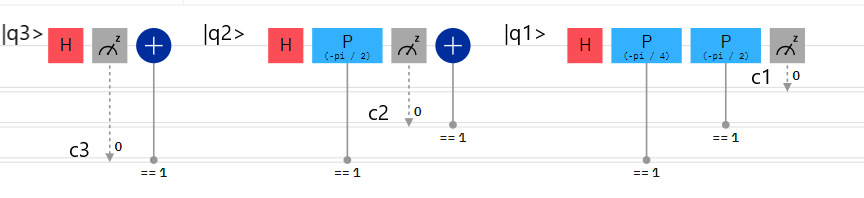
\includegraphics[scale = 0.6]{iterative_iqft.PNG}
  \caption{3 Messungen inverse iterative QFT}
  \label{fig:iterative_iQFT}
\end{figure}
  
Wie im vorherigen Absatz erwähnt, 
werden bei der iterativen Quantum"=Phase"=Estimation die \(U^{2^x}\)-Gatter zwischen den Abschnitten 
der iterativen Quanten"=Fourier"=Transformation angewendet. 

Als Ergebnis besitzt der Quantenschaltkreis für den Shor Algorithmus mit der iterativen Quantum-Phase-Estimation eine grundlegend andere Struktur 
im Vergleich zur regulären Variante.
Dies resultiert darin, dass die iterative Quanten-Fourier-Transformation kein zusammenhängender Baustein ist, 
sondern dass die einzelnen Bestandteile schrittweise zwischen 
den einzelnen \(U^{2^x}\)-Gatter angewendet werden.

\bigskip

Aufgrund der benötigten klassisch-kontrollierten Phasen-Gatter wird die iterative Quanten-Fourier-Transformation nicht als einzelne Gatter, 
sondern in einer Funktion \mintinline{python}{iterative_QFT} definiert.
Diese Funktion wendet die erforderlichen klassisch"=kontrollierten Gatter direkt auf den Quantenschaltkreis für ein jeweiliges Qubit an.

Wie im Code in Abbildung~\ref{code:iterativeQFT} dargestellt, 
erwartet die Funktion \mintinline{python}{iterative_QFT} die vier Parameter: \mintinline{python}{target}, \mintinline{python}{qc}, \mintinline{python}{k} und \mintinline{python}{controlling_qubit}.
Der Parameter \mintinline{python}{target} beschreibt die Wertigkeit des Qubits und 
definiert zusammen mit der Genauigkeit \mintinline{python}{k}, 
welche Phasen-Gatter benötigt werden.
Alle durch die Funktion \mintinline{python}{iterative_QFT} angewendeten Gatter 
werden auf den Quantenschaltkreis im Parameter \mintinline{python}{qc} angewendet.
Der letzte Parameter, \mintinline{python}{controlling_qubit}, beinhaltet das Ziel der angewendeten Gatter und 
somit die Position des Kontrollqubit.

Wenn der Parameter \mintinline{python}{target} dem Wert 0 entspricht, 
wird die iterative Quanten-Fourier-Transformation für das Most-Significant-Bit angewendet.
Wie in Abbildung~\ref{fig:iterative_iQFT} gezeigt, entspricht dies nur der Anwendung eines einzelnen Hadamard-Gatters.
In Zeile 3 und 4 ist zu erkennen, 
dass mit abnehmender Wertigkeit eines Qubits zunehmend mehr Phasen-Gatter angewendet werden.
Alle Phasen-Gatter, welche in Zeile 4. genutzt werden, 
wirken auf das \mintinline{python}{controlling_qubit} und 
werden von unterschiedlichen klassischen Bits mit der Methode \(c_if\) kontrolliert.

Da die Funktion direkt auf den Quantenschaltkreis \mintinline{python}{qc} wirkt, 
wird kein Rückgabewert benötigt.
\begin{listing}[H]
\begin{minted}[linenos,fontsize=\footnotesize]{python}    
def iterative_QFT(target: int, qc: QuantumCircuit ,k: range, controlling_qubit: int):
    if target != 0:
        for i in list(reversed(range(target))):
            qc.p((-pi/(2**(i+1))),controlling_qubit).c_if(k[target - (i+1)],1)
    qc.h(controlling_qubit)
  \end{minted}
  \caption{Part Iterative QFT in Qiskit}
  \label{code:iterativeQFT}
\end{listing}

Der Code zum vollständigen Quantenschaltkreis ist in Abbildung~\ref{code:IterativeQPE} in der Funktion \mintinline{python}{Shor_sequential} dargestellt.
Die Parameter sind identisch mit denen der regulären \mintinline{python}{Shor} Funktion. 
Wie in Zeile 6. der Quantenschaltkreis-Definition zu erkennen ist, 
benötigt diese Variante insgesamt \(2n+3\) Qubits und halbiert damit fast den Bedarf der Standardvariante von \(4n+2\) Qubits.
In den Zeilen 8 bis 14 ist ersichtlich, 
dass die Komponenten der iterativen Quanten-Fourier-Transformation in jedem Schleifendurchlauf nach einem \(U^{2^x}\)-Gatter angewendet werden. 
Des Weiteren ist ersichtlich, 
dass die Schleife mit dem Qubit beginnt, 
welches die höchste Wertigkeit (Most-Significant-Bit) hat.
Pro Iteration wird jeweils ein \(U^{2^x}\)-Gatter mit absteigender Potenzen zum vorherigen Durchlauf angewendet, 
hingegen werden die Messergebnisse in klassischen Bits mit aufsteigender Wertigkeit gespeichert.

\begin{listing}[H]
\begin{minted}[linenos,fontsize=\footnotesize]{python}    
def Shor_sequential(a:int, N:int, number_shots:int=1000,
    backend:str="aer_simulator"):
  n = N.bit_length()
  controlling_qubit = 0
  ev_qbits  = range(1, 2*n+3)
  k = range(2*n)
  qc = qiskit.QuantumCircuit(2*n+3, 2*n) 
  qc.x(1)
  for target in k:
    qc.h(0)
    qc.append(
      U_gate(n,dezToBin(mod_exp(a, 2**(len(k)-target-1), N),n+1),dezToBin(N,n+1)),
      [0]+list(ev_qbits)
    )
    iterative_QFT(target,qc,k,controlling_qubit)
    qc.measure(controlling_qubit,k[target])
    qc.x(0).c_if(k[target],1)
  simulator = qiskit.Aer.get_backend(backend)
  sim_result = qiskit.execute(qc, backend=simulator, shots=number_shots).result()
  return sim_result.get_counts(qc)
  \end{minted}
  \caption{Iterative QPE}
  \label{code:IterativeQPE}
\end{listing}

Für \(a = 7,~N=15,~k=4\) ist in Abbildung~\ref{fig:iterative_iQPE_qiskit} der Quantenschaltkreis nach der Funktion \mintinline{python}{Shor_sequential} dargestellt.
Das \(k\) wurde verringert, damit die Grafik nicht zu viel Platz beansprucht.
Aufgrund des geringeren \(k\) kommen dementsprechend weniger \(U^{2^x}\)-Gatter zum Einsatz.

\begin{figure} [H]
  \centering
  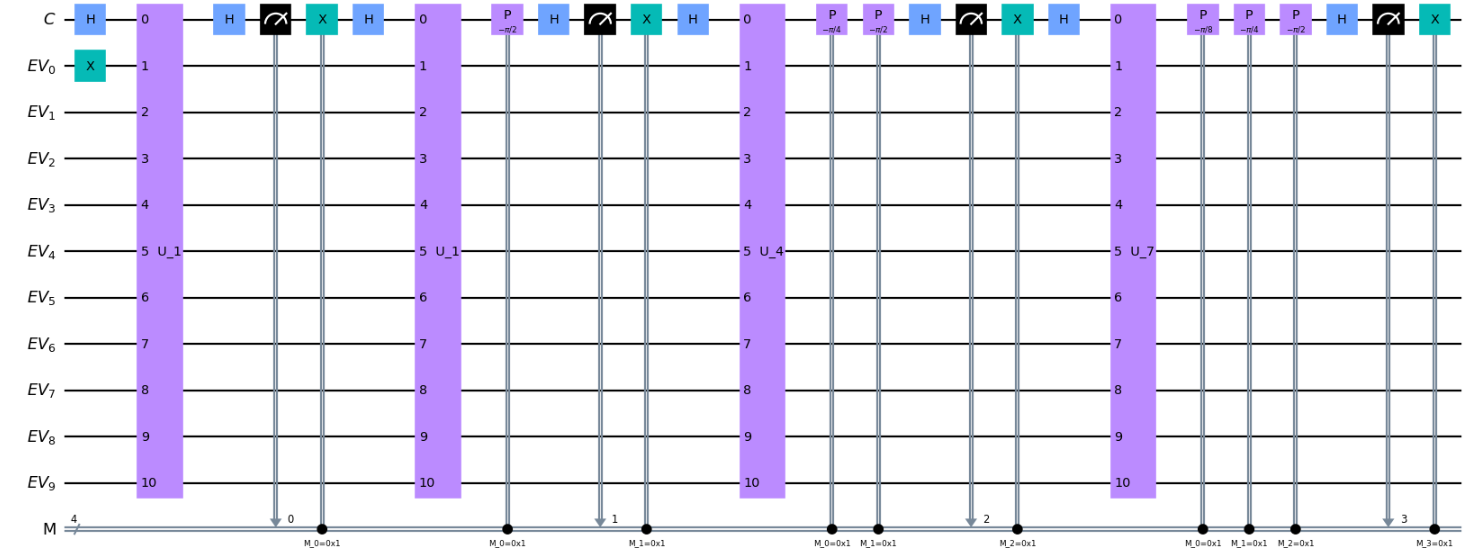
\includegraphics[scale = 0.4]{code_iterative_QPE_qiskit.PNG}
  \caption{iterative QPE Beispiel in qiskit}
  \label{fig:iterative_iQPE_qiskit}
\end{figure}

Der ausschlaggebende Vorteil der iterativen Quantum-Phase-Estimation besteht darin, 
dass diese Variante im Vergleich zur zuvor in Sektion~\ref{section:imp_QPE_Shor} implementierten Variante den Ressourcenbedarf von \(4n+2\) Qubits auf \(2n+3\) Qubits reduziert.

Ein weiterer Vorteil dieser Variante ist, 
dass die Genauigkeit \(k\) nicht auf Kosten von weiteren Qubits erhöht wird, 
sondern ausschließlich durch zusätzliche Gatter.
Deswegen benötigt diese Variante stets \(2n+3\) Qubits, 
sodass der Bedarf an Qubits lediglich von der Größenordnung der Zahl \(N\) abhängig ist.

Der Nachteil der iterativen Variante besteht darin, 
dass die einzelnen Episoden der semi-klassischen Quanten-Fourier-Transformation nicht parallel angewendet werden können.
Hingegen ist es möglich, die regulären inverse Quanten-Fourier-Transformation, bis zu einem gewissen Grad, 
parallel Anzuwenden.
Da dies aber lediglich die letzte Anwendung der Quanten-Fourier-Transformation im Quantum-Phase-Estimation Algorithmus betrifft, 
ist diese zusätzliche Laufzeit vernachlässigbar.

Da sowohl bei der regulären als auch bei der iterativen Variante, 
alle \(U^{2^x}\)-Gatter auf dasselbe Quantenregister wirken, 
können diese nur sequenziell angewendet werden.

Zusammengefasst tauscht man bei der Verwendung der iterativen Variante, 
einen breiteren Quantenschaltkreis gegen einen minimal tieferen ein.

Welche der beiden Varianten vorzuziehen ist, 
hängt vor allem von den zur Verfügung stehenden Ressourcen des Quantencomputers ab.

\bigskip

Die Konstruktion der iterativen Anwendung nach Beauregard ist in Abbildung~\ref{fig:iterative_iQPE_Beauregard} dargestellt.
Anhand der Grafik ist erkennbar, 
dass sowohl die Anwendung der \(U^{2^x}\)-Gatter als auch die Messungen der Qubits in Reihenfolge einer aufsteigenden Wertigkeit geschieht.
Die Anwendung der Gatter und Messungen in dieser Reihenfolge stimmt nicht mit anderen Quellen überein~\cite{Parker2000}.

\begin{figure}[H]
  \centering
  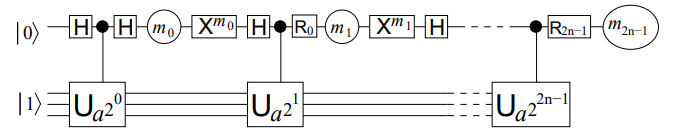
\includegraphics[scale = 0.6]{beauregard_iterative_QPE.png}
  \caption{iterative QPE nach Beauregard~\cite{beauregard2003circuit}}
  \label{fig:iterative_iQPE_Beauregard}
\end{figure}

Wie in Abbildung~\ref{fig:iQFTswaps} für die inverse Quanten-Fourier-Transformation zu sehen ist, 
werden die Gatter auf den Eingangszustand \(\ket{q1}\) durch die Ergebnisse der beiden anderen Kontrollqubits kontrolliert.
Für die iterative Variante nach Beauregard bedeutet das, 
dass die klassisch kontrollierten Phasen-Gatter auf \(\ket{q1}\) von klassischen Bits kontrolliert werden, 
welche noch nicht das Messergebnis beinhalten.
Derselbe Effekt tritt auch für die weiteren Qubits auf.

Ein Nachbau des iterativen Quantenschaltkreises nach Beauregard wie in Abbildung~\ref{fig:iterative_iQPE_Beauregard_qiskit} für \(a = 7,~N=15,~k=4\), 
konnte die Funktionsweise in Simulationen nicht bestätigen.
\begin{figure}[H]
  \centering
  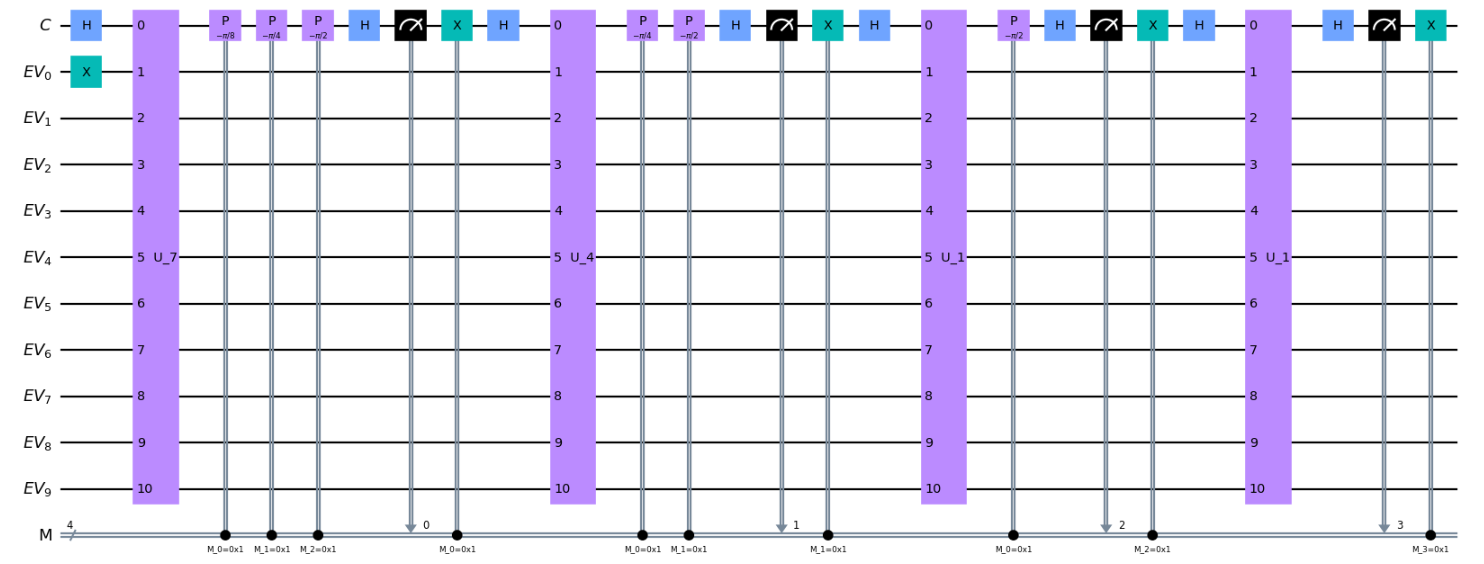
\includegraphics[width=\textwidth]{beauregard_iterative_QPE_qiskit.PNG}
  \caption{iterative QPE Beispiel nach Beauregard}
  \label{fig:iterative_iQPE_Beauregard_qiskit}
\end{figure}
Der Vergleich beider Quantenschaltkreise wird in Abbildung~\ref{fig:iterative_iQPE_Vergleich} dargestellt.
Links sind die Ergebnisse des Quantenschaltkreises aus Abbildung~\ref{fig:iterative_iQPE_qiskit}, 
rechts die des Quantenschaltkreises nach Abbildung~\ref{fig:iterative_iQPE_Beauregard_qiskit}.
Beide Quantenschaltkreise sind für \(a = 7,~N=15,~k=4\) nachgebildet.
Lediglich das Ergebnis auf der linken Seite ist korrekt, 
da die Messergebnisse übereinstimmen, 
als auch genau vier Peaks vorhanden sind, 
was der Länge der Periode entspricht.
\begin{figure}[H]
  \centering
  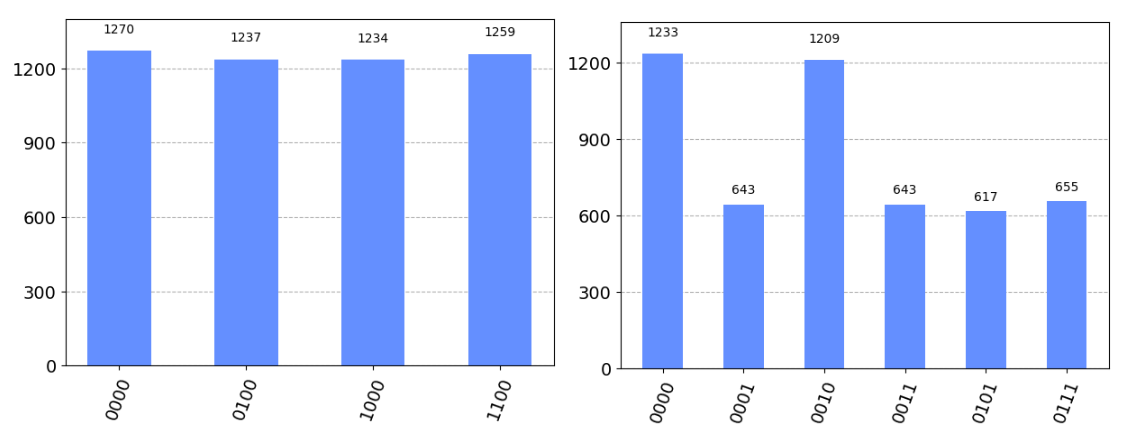
\includegraphics[scale = 0.4]{Vergleich_interative_QPE.png}
  \caption{iterative QPE Messergebnisse(Beauregard rechts)}
  \label{fig:iterative_iQPE_Vergleich}
\end{figure}

Um ein Missverständnis auszuschließen, wurde versucht, Stéphane Beauregard zu kontaktieren. 
Leider waren keine Kontaktinformationen auf den Portalen hinterlegt, 
auf denen seine Arbeiten öffentlich zugänglich sind. 
Die einzige nützliche Information, die dabei gefunden wurde, 
war seine Zugehörigkeit zur University of Montreal. 
Auf LinkedIn wurde ein anderer Stéphane Beauregard gefunden, 
der zufällig auch an der University of Montreal war. Auf Nachfrage wurde jedoch herausgefunden, 
dass es sich um eine andere Person handelt. 
Eine Anfrage bei der University of Montreal selbst war aus Datenschutzgründen erfolglos. 
Als letzte Option wurde der häufigste Co-Autor kontaktiert. 
Der Co-Autor Guy Lapalme ist emeritierter Professor der University of Montreal.
Da Beauregard die University of Montreal verlassen hat, 
hatte auch Guy Lapalme keine Kontaktinformationen von Beauregard.

\bigskip

Im Faktorisierungsalgorithmus wird die iterative Quantum-Phase-Estimation genutzt, 
wenn die Anzahl der erforderlichen Qubits für die reguläre Variante mit \(4n+2\) Qubits einen zu hohen Ressourcenbedarf darstellt, 
den der genutzte Quantencomputer nicht bereitstellen kann. 
In diesem Fall wird auf Kosten der Laufzeit die sparsamere Variante angewendet. 
Sollten auch dafür nicht genügend Qubits vorhanden sein, 
wird die Berechnung mit einer Fehlermeldung abgebrochen. 
Die Fallunterscheidung in der Implementierung wird realisiert, 
indem statt der Funktion \mintinline{python}{Shor} die iterative Variante \mintinline{python}{Shor_sequential} ausgeführt wird. 
Weitere Anpassungen sind nicht nötig, 
da sowohl die Eingabewerte als auch die Form der Rückgabewerte identisch sind.

\subsubsection{Approximative Quanten-Fourier-Transformation} \label{sec:ApproxQFT}
Die zweite Methode zur Ressourceneinsparung betrifft ebenfalls die Quanten-Fourier-Transformation und 
wurde erstmals 1996 vorgestellt~\cite{Barenco_1996}.
Bei dieser Optimierung wird die Ressourceneffizienz durch die Reduktion der verwendeten Gatter erreicht. 
Sowohl die reguläre als auch die iterative Quanten-Fourier-Transformation verwenden (klassisch) kontrollierte Phasen-Gatter.
Dabei kommen Phasenverschiebungen im Bereich von \(e^{\frac{2\pi i}{2^1}}\) bis \(e^{\frac{2\pi i}{2^n}}\) zur Anwendung. 
Dies führt zu einem exponentiellen Wachstum der Zweierpotenz im Nenner des Bruchs der wirkenden Phasenverschiebung, 
was wiederum eine exponentielle Abnahme der wirkenden Phasenverschiebungen bei jedem weiteren Phasen-Gatter bewirkt. 

Die approximative Quanten-Fourier-Transformation nutzt den Effekt aus, 
dass die Beiträge höherer Phasen-Gatter für das Endergebnis oft weniger kritisch sind, 
um eine reduzierte Anzahl an Gattern einzusetzen. 
Indem ein angemessener Approximationsfaktor gewählt wird, 
kann eine Genauigkeit erzielt werden, 
die weiterhin für ein akzeptables Endergebnis ausreichend ist.

Die approximative Quanten-Fourier-Transformation wird als \(\AQFT_m\) definiert und 
wendet maximal \(m\) Phase-Gatter pro Qubit an. 
Der Parameter \(m\) wird als Approximationsfaktor bezeichnet und bestimmt die Präzision der \(\AQFT_m\). 
Der Approximationsfaktor gibt an, 
bis zu welcher Phasenverschiebung von \(e^{\frac{2\pi i}{2^m}}\) die Phasen-Gatter angewendet werden.
Die vollständige Quanten-Fourier-Transformation entspricht einer \(\AQFT_n\).

Wenn der Approximationsfaktor \(m\) einen Wert
\[m \geq \ld(n)+2\]
entspricht, nähert sich die Wahrscheinlichkeit, das optimale Ergebnis mit \(\AQFT_m\)
zu erhalten, dem Wert~\cite{cheung2004improved}: 
\[P \geq \frac{4}{\pi^2} - \frac{1}{4n}\]
Dies steht im Gegensatz zur Wahrscheinlichkeit von \(\frac{4}{\pi^2}\), 
die für die exakte Quanten-Fourier-Transformation \(\QFT\) gilt~\cites{cheung2004improved}[119]{kaye2007introduction}.

Im Hinblick auf die Ressourceneffizienz benötigt die \(\AQFT_m\) insgesamt \(\Landau(nm)\) Gatter.
Wenn \(m\) wie zuvor definiert wird, entspricht dies \(\Landau(n~\ld(n))\). 
Im Vergleich dazu erfordert die exakte Quanten-Fourier-Transformation \(\Landau(n^2)\) Gatter~\cite{Barenco_1996}.
Die Tiefe der Schaltung wird durch die approximative Quanten-Fourier-Transformation im Vergleich zur exakten nicht verändert.

Daraus folgt, dass die approximative Quanten-Fourier-Transformation einen effizienteren Bedarf an Gattern aufweist, 
jedoch zulasten einer geringeren Genauigkeit im Vergleich zur exakten Quanten-Fourier-Transformation.
Aufgrund der identischen Tiefe beider Varianten ist die Laufzeit beider Varianten ebenfalls identisch.

Allerdings gilt dies nur unter der Annahme, 
dass der Quantencomputer ideal ist und weder Dekohärenzeffekte noch andere Fehler aufweist.
Im Falle eines idealen Quantencomputers liefert die exakte Quanten-Fourier-Transformation, die alle Phasen-Gatter anwendet, 
mit höherer Wahrscheinlichkeit ein genaues Ergebnis als die approximative Quanten-Fourier-Transformation.

Wenn allerdings kein idealer Quantencomputer genutzt wird, 
führt die Dekohärenz, 
bedingt durch eine Vielzahl an Gattern, 
zu einer erhöhten Fehlerrate.
Eine Reduktion der Anzahl an Gattern durch ein geringeres 
\(m\) führt daher zu einer niedrigeren Fehlerrate durch Dekohärenz, 
was wiederum die Wahrscheinlichkeit für ein genaues Ergebnis erhöht.
Auf der anderen Seite führt ein geringeres \(m\) zu einer Ungenauigkeit,
da der Approximationsfaktor größer ist und somit nicht alle Phasen-Gatter angewendet werden.
Um das bestmögliche Ergebnis zu erzielen, 
muss eine gewisse Ungenauigkeit durch die Approximation in Kauf genommen werden, 
die wiederum durch die geringere Fehlerrate kompensiert wird. 
Das optimale \(m\) nähert sich der Untergrenze von~\cite{Barenco_1996}:
\[m \geq \ld(n)+2\]

Die Approximationstechnik kann auch in der iterativen beziehungsweise, 
semi"=klassisch\-en Quanten-Fourier-Transformation angewendet werden. 
Bei der Implementierung für den Shor-Algorithmus ist darauf zu achten, 
dass alle verwendeten Quanten"=Fourier"=Transformationen, also sowohl die in den \(U^{2^x}\)-Gattern als auch die finale Transformation vor dem Basiswechsel, 
das gleiche \(m\) nutzen.
Andernfalls wären die angewendeten und extrahierten Phasenverschiebungen inkonsistent 
und würden zu falschen Ergebnissen führen.

Die Implementierung des \mintinline{python}{Faktorisierungsalgorithmus} wird um den Parameter \(m\) ergänzt.
Standardmäßig entspricht der Approximationsfaktor 
\[m = \lceil\ld(n)+2\rceil\]  
Dieser kann jedoch über den Parameter beliebig angepasst oder 
durch Setzen von \(m=-1\) deaktiviert werden.
Im Falle der Deaktivierung wird die exakte Quanten-Fourier-Transformation angewendet.

Der Grund, warum die approximative Variante standardmäßigen verwendet wird, 
liegt darin, dass das Ergebnis bereits bei kleinen \(n\) eine gute Genauigkeit gewährt. 
Dies wird deutlich, wenn man Abbildung~\ref{fig:shor_measure} mit \(m=n=7\) und
Abbildung~\ref{fig:shor_measure_AQFT} mit \(m=4\) vergleicht.
Abgesehen von \(m\) sind die Berechnungen in beiden Abbildungen identisch.
Mit steigendem \(n\) nimmt die Ungenauigkeit durch die fehlenden Gatter ab, 
bis sie schließlich ganz vernachlässigbar wird~\cite{cheung2004improved}.

\begin{figure}[H]
  \centering
  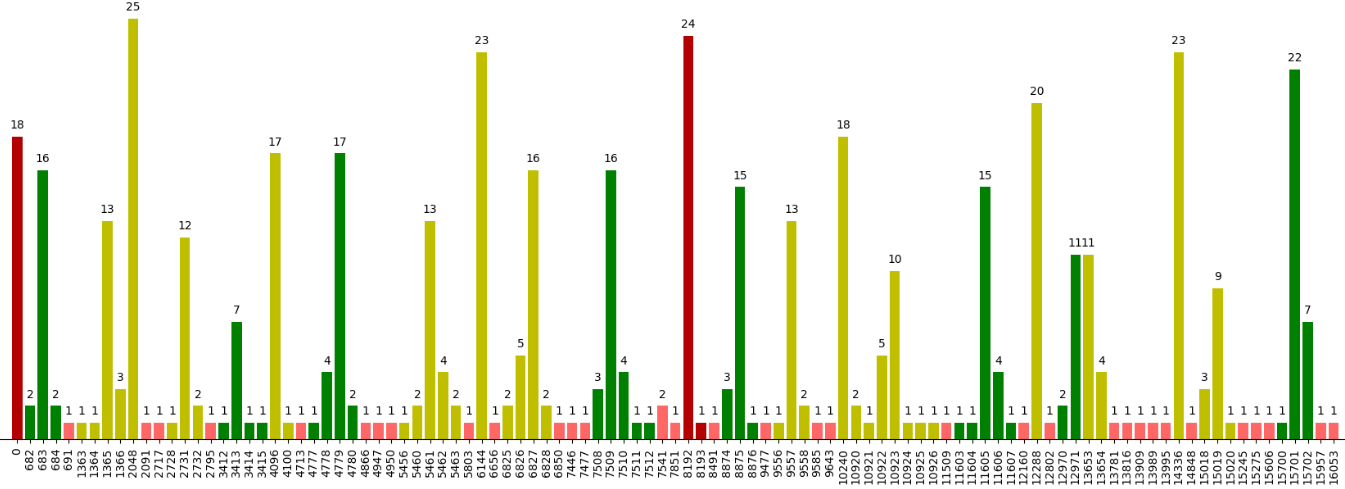
\includegraphics[width=\textwidth]{shor_measure_AQFT.PNG}
  \caption{AQFT Messung a=19, N=119, k=14, m=4}
  \label{fig:shor_measure_AQFT}
\end{figure}

\section{Resultate}
In der nachfolgenden Analyse liegt der Fokus auf der Evaluierung der implementierten Varianten des Shor-Algorithmus hinsichtlich ihres Ressourcenverbrauchs und 
der Laufzeitkomplexität. 
Angesichts der signifikanten Auswirkungen des Algorithmus für die Integrität des kryptografischen Systems des RSA-Verfahrens  
orientieren sich die zugrunde gelegten Bewertungskriterien an den Richtlinien für Post-Quantenkryptografie des \textit{National Institute of Standards and Technology}(NIST). 
Die erzielten Resultate ermöglichen eine Einordnung in die Größenordnung der erforderlichen Laufzeit und 
erlauben einen direkten Vergleich mit den Ergebnissen anderer Arbeiten.

\subsection*{Laufzeit}
In der Publikation "'Submission Requirements and Evaluation Criteria for the Post-Quantum Cryptography Standardization Process"` des NIST~\cite[17]{NISTPQC} 
werden drei Sicherheitsstufen definiert, die sich auf die Laufzeitanforderungen von Quantencomputern in Bezug auf kryptografische Angriffe beziehen.

Als Metrik für die Laufzeitevaluation wird der Parameter \textit{Maxdepth} eingeführt, 
welcher die Anzahl der Quantengatter für die längste serielle Ausführung eines Quantenalgorithmus erfasst.
Die Auswahl dieser Metrik wird in der Publikation damit begründet, dass lange serielle Berechnungen Herausforderungen mit sich bringen.

Die schwächste der drei Sicherheitsstufen beginnt bei einer \textit{Maxdepth} von \(2^{40}\) Quantengattern. 
Dieser Wert dient als approximative Messgröße für die Anzahl an seriell ausgeführten Quantengattern, 
die nach aktueller Prognose von Quantencomputern innerhalb eines Jahres realisiert werden können.

Die nächste Sicherheitsstufe setzt eine \textit{Maxdepth} von \(2^{64}\) Quantengattern an.
Dieser Wert stellt die approximative Anzahl an seriell ausgeführten Quantengattern dar, 
die nach der Prognose innerhalb eines Jahrzehnts durchgeführt werden können.

Die stärkste Sicherheitsstufe ist bei einer \textit{Maxdepth} von \(2^{96}\) Quantengattern festgelegt. 
Selbst unter idealen Bedingungen, 
bei denen Qubits auf atomarer Skala arbeiten und die Übertragungsgeschwindigkeit der Lichtgeschwindigkeit entspricht, 
würde diese Anzahl an Quantengattern ein Jahrtausend an Berechnungszeit erfordern.


\subsection*{Ressourcenbedarf}
Als Metriken für den Ressourcenverbrauch werden die benötigte Anzahl an Qubits sowie die Gesamtanzahl an Quantengattern herangezogen. 
Die Anzahl der Qubits stellt eine notwendige Voraussetzung dar, 
die ein Quantencomputer erfüllen muss, da andernfalls die Ausführung des Quantenalgorithmus nicht möglich ist. 
Die Gesamtanzahl an Quantengattern dient als eine Kennzahl, 
die potenzielle Rückschlüsse auf die Fehlerrate durch Dekohärenz zulässt. 
Darüber hinaus finden sowohl die Anzahl an Qubits als auch die Gesamtanzahl an Quantengattern häufig Anwendung als Kennzahl in der wissenschaftlichen Literatur. 
Diese beiden Metriken ermöglichen somit einen Vergleich mit den Ergebnissen anderer Arbeiten.

In der Analyse wurden ausschließlich elementare Quantengatter wie Hadamard-, Phasen- und X-Gatter in die Betrachtung einbezogen. 
Die in Sektion~\ref{sec:Implementierung} eingeführten, spezialisierten Gatter wurden nicht direkt gezählt, 
stattdessen wurden die darin enthaltenen Basisgatter gezählt. 
Dieses Vorgehen ergibt sich aus der Tatsache, dass ein Quantencomputer effektiv die Basisgatter eines Quantenschaltkreises ausführt. 
Übergeordnete, spezialisierte Gatter werden demzufolge in ihre elementaren Komponenten zerlegt. 
Eine Zählung der spezialisierten Gatter wäre somit nicht repräsentativ für die tatsächliche Ressourcennutzung.

Für die Zählung der Anzahl der Gatter sowie der \textit{Maxdepth} des Quantenschaltkreises wurden spezifische Funktionen der Qiskit-Bibliothek genutzt. 
Diese Funktionen erlauben die Bestimmung der Anzahl an Gatter und der \textit{Maxdepth} in einem Quantenschaltkreis.
Dabei ist zu beachten, dass diese Funktionen keine Unterscheidung zwischen elementaren und spezialisierten Gattern treffen.
Daher konnte die Funktionen nicht direkt zur Analyse des vorliegenden Quantenschaltkreises verwendet werden. 
Als Lösungsansatz wurde der Code zur Zählung modifiziert, um sicherzustellen, dass der Quantenschaltkreis ausschließlich aus Basisgattern besteht.

\subsection*{Analyse}
Die Analyse beinhaltet eine Untersuchung von vier Varianten des Shor-Algorithmus, 
die jeweils unterschiedliche Kombinationen der in Sektion~\ref{Optimierung} erörterten Optimierungsstrategien implementieren.
Die vier Varianten werden nach den implementierten Optimierungsstrategien in die Kategorien \textit{Reguläre}, 
\textit{Approximative}, \textit{Iterative} und \textit{Approximative-Iterative} eingeteilt.
In den Kategorien unterscheidet sich insbesondere die Nutzung der Quantum-Phase-Estimation und der Quanten-Fourier-Transformation. 
Während die \textit{Reguläre} Variante auf die \(4n+2\) Qubit Version der Quantum-Phase-Estimation mit der exakten Quanten-Fourier-Transformation setzt, 
nutzt die \textit{Approximative} Variante ebenfalls die \(4n+2\) Qubit Variante, 
verwendet jedoch die approximative Quanten-Fourier-Transformation mit einem Approximationsfaktor von \(m = \lceil\text{ld}(n)+2\rceil\).

Die \textit{Iterative} Variante bedient sich der iterativen Quantum-Phase-Estimation mit \(2n+3\) Qubits und 
verwendet die exakte Quanten-Fourier-Transformation, dementsprechend in iterativer Anwendung.
Die \textit{Approximative-Iterative} Variante verwendet ebenfalls die iterative Quantum-Phase-Estimation mit \(2n+3\) Qubits, 
aber ergänzt die iterativ angewendete Quanten-Fourier-Transformation um einen Approximationsfaktor von \\\(m = \lceil\text{ld}(n)+2\rceil\).

Die Analyse bezieht sich auf die Schlüssellängen des RSA-Kryptosystems von 1024-Bit, 2048-Bit, 3072-Bit und 4096-Bit. 
Nach aktuellem Stand empfiehlt das BSI für das RSA-Verfahren keine Schlüssellänge unter 3000-Bit~\cite[41]{BSI2023}. 
Nichtsdestotrotz sind heutzutage noch immer Varianten des RSA-Kryptosystems in Einsatz, welche kürzere Schlüssel verwenden, 
weshalb diese ebenfalls berücksichtigt werden.

\vspace{1em}

\begin{table}[H] \label{Varainten_Analyse}
    \centering
    \caption{Vergleich der vier Varianten des Shor-Algorithmus für verschiedene Schlüssellängen}
    \begin{tabular}{|l|l|l|l|l|}
        \hline
        \textbf{Variante} & \textbf{Schlüssellänge} & \textbf{Qubits} & \textbf{Gatteranzahl} & \textbf{Maxdepth} \\ \hline
        Reguläre & 1024-Bit & 4098 & \(2^{43}\) & \(2^{35}\) \\ \hline
        Reguläre & 2048-Bit & 8194 & \(2^{47}\) & \(2^{38}\) \\ \hline
        Reguläre & 3072-Bit & 12290 & \(2^{49}\) & \(2^{40}\) \\ \hline
        Reguläre & 4096-Bit & 16386 & \(2^{51}\) & \(2^{41}\) \\ \hline
        Approximative & 1024-Bit & 4098 & \(2^{38}\) & \(2^{35}\) \\ \hline
        Approximative & 2048-Bit & 8194 & \(2^{41}\) & \(2^{38}\) \\ \hline
        Approximative & 3072-Bit & 12290 & \(2^{43}\) & \(2^{40}\) \\ \hline
        Approximative & 4096-Bit & 16386 & \(2^{44}\) & \(2^{41}\) \\ \hline
        Iterative & 1024-Bit & 2051 & \(2^{43}\) & \(2^{35}\) \\ \hline
        Iterative & 2048-Bit & 4099 & \(2^{47}\) & \(2^{38}\) \\ \hline
        Iterative & 3072-Bit & 6147 & \(2^{49}\) & \(2^{40}\) \\ \hline
        Iterative & 4096-Bit & 8195 & \(2^{51}\) & \(2^{41}\) \\ \hline
        Approximative-Iterative & 1024-Bit & 2051 & \(2^{38}\) & \(2^{35}\) \\ \hline
        Approximative-Iterative & 2048-Bit & 4099 & \(2^{41}\) & \(2^{38}\) \\ \hline
        Approximative-Iterative & 3072-Bit & 6147 & \(2^{43}\) & \(2^{40}\) \\ \hline
        Approximative-Iterative & 4096-Bit & 8195 & \(2^{44}\) & \(2^{41}\) \\ \hline
    \end{tabular}
    \end{table}
    
Anhand der Tabelle~\ref{Varainten_Analyse} fällt auf,
dass die unterschiedlichen Varianten keinen Unterschied in Bezug auf die \textit{Maxdepth} haben.
Stattdessen ist die Schlüssellänge der einzige Faktor, 
der die \textit{Maxdepth} beeinflusst.

Hingegen ermöglicht der Einsatz eines approximativen und iterativen Ansatzes deutliche Einsparungen im Hinblick auf den Ressourcenbedarf. 
Im Vergleich zu einer Schlüssellänge von 4096-Bit ermöglicht die Verwendung der approximativen Quanten-Fourier-Transformation im Vergleich zur exakten Variante eine Reduzierung der Gesamtanzahl an Gattern um etwa den Faktor 100.
Wie in Sektion~\ref{sec:ApproxQFT} erwähnt, ist der Genauigkeitsverlust durch die approximative Variante für große \(N\) vernachlässigbar. 
Des Weiteren schneidet die approximative Variante in Anwesenheit von Dekohärenz aufgrund der geringeren Anzahl an Gattern besser ab~\cite{Barenco_1996}. 
Diese Aspekte sprechen dafür, den approximativen Ansatz grundsätzlich vorzuziehen.

\subsection*{Vergleich}
In Abschnitt~\ref{sec:QuantumAdder} wurde erläutert, 
dass die Verwendung klassischer Volladdierer in einem Quantenschaltkreis mehr Ressourcen erfordert als die Nutzung der Quantum-Addition. 
Da der Baustein zur Addition in Shors Algorithmus häufig vorkommt, 
hat dies dementsprechend einen erheblichen Einfluss auf den Gesamtressourcenbedarf.

Um eine Abwägung beider Methoden durchzuführen, 
werden die Ergebnisse der Analyse mit dem berechneten Ressourcenbedarf aus der Publikation "'Estimation of Shor’s Circuit for 2048-bit Integers
based on Quantum Simulator"`~\cite{cryptoeprint:2023/092} verglichen. 
Diese Publikation untersucht den Ressourcenbedarf für einen ähnlichen Ansatz zur Implementierung des Shor-Algorithmus.
Der entscheidende Unterschied besteht darin, 
dass der in dieser Publikation verwendete Quantenschaltkreis klassische Volladdierer nach der Anleitung von 
\textit{Vedral}, \textit{Barenco} und \textit{Ekert}\cite{Vedral_1996} verwendet.

In Tabelle~\ref{Volladdierer_Analyse} sind die Ergebnisse der Publikation dargestellt:

\begin{table}[H] \label{Volladdierer_Analyse}
    \centering
    \caption{Vergleich Shor-Algorithmus mit Volladdierer~\cite{cryptoeprint:2023/092}}
    \begin{tabular}{|l|l|l|l|l|}
        \hline
        \textbf{Variante} & \textbf{Schlüssellänge} & \textbf{Qubits} & \textbf{Gatteranzahl} & \textbf{Maxdepth} \\ \hline
        Volladdierer & 1024-Bit & 5121 & \(2^{38}\) & \(2^{38}\) \\ \hline
        Volladdierer & 2048-Bit & 10241 & \(2^{41}\) & \(2^{41}\) \\ \hline
    \end{tabular}
\end{table}
In der Publikation werden die Ressourcen nur für Schlüssellängen von jeweils \(1024\) und \(2048\) Bit untersucht. 
Nichtsdestotrotz lässt sich im direkten Vergleich feststellen, 
dass die Verwendung der Quanten-Addition in allen Fällen zu einer geringeren \textit{Maxdepth} führt. 
Darüber hinaus wird der zusätzliche Bedarf an Qubits bei Verwendung von Volladdierer offensichtlich. 
Lediglich im Gesamtbedarf an Quantengattern schneidet die Variante mit Volladdierer besser ab als die Varianten, 
welche die exakte Quanten-Fourier-Transformation nutzen. 
Andererseits weist der approximative Ansatz einen äquivalenten Gesamtbedarf an Quantengattern zur Variante mit Volladdierer auf.

\subsection*{Effekt der Nachberechnung}

Bezüglich der \textit{Maxdepth} erfüllt eine Schlüssellänge von mindestens, 
3072 Bit bereits die Kriterien der geringsten Sicherheitsstufe. 
Es ist jedoch zu beachten, dass diese \textit{Maxdepth} nur für einen einzelnen Durchlauf des Quantenalgorithmus gilt. 
Wenn mehrere Durchläufe benötigt werden, steigt dementsprechend auch die \textit{Maxdepth} der gesamten Berechnung.

Wie in Sektion~\ref{Funktionsweise:klassisch} erklärt, kann es ohne klassische Nachberechnungen bis zu \(2\text{ld}(N)\) Messungen erfordern, 
bis ein Messergebnis die ungekürzte Periode enthält. 
In Bezug auf eine Schlüssellänge von 3072 Bit würde das im Worst-Case-Szenario \(2\text{ld}(2^{3072})\) erfordern, 
also in etwa \(2^{13}\) Durchläufe des Quantenalgorithmus.
Dies ergibt eine gesamte \textit{Maxdepth} aller Durchläufe von \(2^{40} \cdot 2^{13}\), insgesamt also \(2^{53}\).
Unter Berücksichtigung der erforderlichen Laufzeiten wird die Sinnhaftigkeit intensiver Nachberechnungen mit klassischen Methoden verdeutlicht.

Um einen Vergleich zwischen den benötigten Durchläufen mit Nachberechnung und den Durchläufen ohne Nachberechnung zu ermöglichen, 
wurden die Erfolgsraten beider Methoden erhoben.

Dazu wurden beide Methoden verwendet, um die Zahl \(N=391\) jeweils 200-mal zu faktorisieren.
Die Statistik beinhaltet die Anzahl an benötigten Durchläufe des Quantenalgorithmus, die pro Faktorisierung notwendig waren.

Die Berechnung des Quantenalgorithmus wurde unter Verwendung des Simulators von Qiskit durchgeführt. 
Bei jedem Durchlauf wurde ein zufälliges \(a\) gewählt.
Um die Statistik nicht zu verfälschen, wurden Durchläufe, die ein \(a\) verwendeten, 
welches ein Faktor von \(N\) war, nicht gezählt.

Beide Methoden verwendeten die Approximative-Iterative Variante des Quantenalgorithmus mit einem \(k=2n\) und \(m=\lceil\text{ld}(n)+2\rceil\).
Dies entspricht den beiden Standardwerten, 
wie in der Implementierung in Sektion~\ref{sec:Implementierung} verwendet wurde. 
Die Nachberechnung wurde nach dem Verfahren, wie in Sektion~\ref{sec:Faktorisierungsalgorithmus} beschrieben, angewendet. 
Die Anzahl der zu überprüfenden Nachbarn und Vielfachen in der klassischen Nachberechnung betrug ebenfalls den standardmäßigen Wert von \(2^{\text{ld}(\text{ld}(N))}\).

\begin{table}[h] \label{Nachberechnung}
    \centering
    \caption{Anzahl der Durchläufe pro Faktorisierung mit Nachberechnung}
    \begin{tabular}{|c|c|c|c|c|c|c|} 
        \hline
        \textbf{Durchläufe} & 1 & 2 & 3 & 4\\
        \hline
        \textbf{Häufigkeit} & 168 & 27 & 3 & 2 \\
        \hline
    \end{tabular}
\end{table}

\begin{table}[h] \label{ohneNachberechnung}
    \centering
    \caption{Anzahl der Durchläufe pro Faktorisierung ohne Nachberechnung}
    \begin{tabular}{|c|c|c|c|c|c|c|c|c|c|} 
        \hline
        \textbf{Durchläufe} & 1 & 2 & 3 & 4 & 5 & 6 & 7 & 8 & 11 \\
        \hline
        \textbf{Häufigkeit} & 87 & 51 & 28 & 14 & 9 & 5 & 3 & 2 & 1 \\
        \hline
    \end{tabular}
\end{table}

Im direkten Vergleich der Ergebnisse von Tabelle~\ref{Nachberechnung} zu Tabelle~\ref{ohneNachberechnung} fällt auf, 
dass aufgrund der durchgeführten Nachberechnung häufig nur ein einzelner Durchlauf des Quantenalgorithmus nötig war. 
Hingegen ist bei einem Vorgehen ohne Nachberechnung ein einzelner Durchlauf in weniger als der Hälfte der Fälle ausreichend. 
Des Weiteren war bei der Verwendung einer Nachberechnung nur bei 2.5\% aller Faktorisierungen mehr als zwei Durchläufe nötig. 
Wiederum gab es ohne Nachberechnung in mehr als 30\% der Fälle die Notwendigkeit für mehr als zwei Durchläufe. 
Dazu kommt, 
dass das gemessene Worst-Case-Szenario ohne Nachberechnung um fast Faktor 3 mehr Durchläufe benötigte als das Worst-Case-Szenario bei der Verwendung von Nachberechnungen.

Unter Beachtung der durchschnittlichen Durchläufe pro Faktorisierung beläuft sich der Durchschnittswert mit Nachberechnungen auf \(1,2\). 
Bei einem Vorgehen ohne Nachberechnung sind durchschnittlich \(2,26\) Durchläufe nötig. 
In Bezug auf die \textit{Maxdepth} erhöht das Auslassen einer Nachberechnung diesen Wert um eine Potenz von 2.

Es wurden keine größeren Zahlen zur Auswertung gewählt, 
da die Simulation bereits für diese Größenordnung bei 200 Durchläufen mehrere Tage in Anspruch nahm.

\subsection*{Kritik}

Anhand der in Tabelle~\ref{Varainten_Analyse} aufgeführten \textit{Maxdepth}-Werte lässt sich erkennen, 
dass selbst unter optimalen Bedingungen, bei denen ein einzelner Durchlauf zur Faktorisierung führt, 
der implementierte Quantenalgorithmus für Schlüssellängen ab 3072 Bit eine Laufzeit erfordert, 
die den niedrigsten Sicherheitsanforderungen gemäß den NIST-Kriterien entspricht. 
Dies verdeutlicht, dass die verwendete Implementierung des Quantenschaltkreises in dieser Arbeit, 
keine effiziente Methode darstellt, 
um ein RSA-Verfahren mit den derzeit empfohlenen Schlüssellängen zu kompromittieren.

Stattdessen wird für die effiziente Faktorisierung ein Quantenschaltkreis benötigt, 
der für Schlüssellängen mit mehr als 3072 Bit eine geringere \textit{Maxdepth} als \(2^{40}\) aufweist.

\vspace{1em}

In Abschnitt~\ref{Funktionsweise:klassisch} wurde darauf hingewiesen, 
dass im Grunde genommen ein Wert \(k\) mit \(k > 2\text{ld}(p)\) ausreichend Genauigkeit gewährt.
Ein möglicher Ansatz zur Reduzierung der \textit{Maxdepth} des hier verwendeten Quantenschaltkreises besteht darin, 
auf eine geringere Größenordnung der Periode zu spekulieren, 
um einen Quantenschaltkreis mit einer kleineren \textit{Maxdepth} zu erreichen~\cite{Shor_1997}. 
Zum Beispiel würde ein \(p\) in der Größenordnung von \(2^{1500}\) mit einem entsprechenden \(k = 2\text{ld}(2^{1500})\) dazu führen, 
dass die \textit{Maxdepth} des Quantenschaltkreises von \(2^{40}\) auf \(2^{37}\) reduziert wird. 
Es ist jedoch wichtig zu betonen, dass die Erfolgswahrscheinlichkeit dieses Ansatzes kritisch zu betrachten ist. 
In einem Szenario mit einem Gesamtraum von \(2^{3072}\) ist es äußerst unwahrscheinlich, 
dass eine Periode mit einem kleineren Wert als \(2^{1500}\) vorkommt.
Konkret ist der gesamte Raum um den Faktor \(\frac{2^{3072}}{2^{1500}} = 2^{1572}\) größer als die vermutete Größe der Periode. 
Daher ist die Wahrscheinlichkeit, dass die Periode größer als \(2^{1500}\) ist, 
um einen ähnlichen Faktor höher als die Wahrscheinlichkeit, 
dass sie kleiner als \(2^{1500}\) ist.

\vspace{1em}

Andere Möglichkeiten zur Reduzierung der \textit{Maxdepth} des in dieser Arbeit implementierten Quantenalgorithmus sind nicht bekannt. 
Es liegt nahe anzunehmen, dass für eine effektive Reduktion der \textit{Maxdepth}, ohne signifikante Nachteile, 
eine andere Architektur für einige der verwendeten Bausteine entwickelt werden muss.

\subsection*{Schlussfolgerung}

Daraus lässt sich ableiten, 
dass eine äußerst ressourceneffiziente Implementierung in Bezug auf die Anzahl der benötigten Qubits für die Faktorisierung 
sehr großer \(N\) zu zeitaufwändigen Berechnungen aufgrund einer hohen \textit{Maxdepth} führt. 
Somit ergibt sich die Schlussfolgerung, 
dass der Schwerpunkt bei der Konstruktion des Quantenschaltkreises nicht auf einem möglichst sparsamen Qubit-Bedarf liegen sollte.

Es ist denkbar, dass durch die Verwendung zusätzlicher Qubits ein Quantenschaltkreis mit einer geringeren \textit{Maxdepth} konstruiert werden kann. 
Bei der Konstruktion eines solchen Quantenschaltkreises könnte man sich auf die Parallelisierung der Berechnung konzentrieren. 

Eine weitere potenzielle Einsparmöglichkeit besteht beim Baustein der modularen Addition aus Sektion~\ref{sub:modulareAddition}.
Indem auf die Quantengatter verzichtet wird, 
welche das Bedingungs-Qubit zurücksetzen, 
kann die \textit{Maxdepth} dieses Bausteins um mehr als die Hälfte reduziert werden. 
Anstelle einer Zurücksetzung könnte stattdessen ein neues Qubit verwendet werden. 
Konkrete Ansätze erfordern jedoch eine ausführliche Untersuchung.



\section{Fazit und Ausblick}
\subsection*{Fazit}
Mit dem Ziel, eine Bibliothek von Quantenalgorithmen für die Kryptoanalyse zu entwickeln, 
wurde der Shor-Algorithmus in vier verschiedenen Varianten implementiert. 
Im Verlauf der Arbeit wurde zuerst die Funktionsweise der benötigten Bausteine, 
wie die Quanten-Fourier-Transformation und die Quantum-Phasen-Estimation, erläutert. 
Auf dieser Grundlage wurde die Verbindung zum Shor-Algorithmus hergestellt, 
der in seiner Essenz eine Form der Quantum-Phase-Estimation mit spezifischen unitären Gattern darstellt. 
Im weiteren Verlauf der Arbeit wurde die Funktionsweise und die Implementierung der spezifischen unitären Gatter 
sowie des gesamten Shor-Algorithmus vorgeführt. 

Aufbauend auf der resultierenden Struktur des Shor-Algorithmus wurden zwei Optimierungen angewendet, 
die den Bedarf an Qubits sowie den gesamten Bedarf an Quantengattern signifikant verringern. 
Bei der Untersuchung einer dieser Optimierungen wurde festgestellt, 
dass es einen Fehler in einer der verwendeten Quellen gibt. 
Unter Hinzunahme von Simulationen wurde nachgewiesen, 
dass diese Unstimmigkeit zu einem fehlerhaften Quantenschaltkreis führt.

Des Weiteren wurde ein klassischer Algorithmus entwickelt, 
um die Erfolgsrate des Shor-Algorithmus zu steigern. 
Dieser Algorithmus führt Berechnungen basierend auf den Messergebnissen des Shor-Algorithmus durch und wurde speziell entworfen, 
um auf drei mögliche Sonderfälle eines Messergebnisses zu reagieren. Diese Sonderfälle wurden anhand von Simulationen erläutert.

In einer abschließenden Analyse wurden die vier resultierenden Varianten des Shor-Algorithmus, 
die im Prinzip aus unterschiedlichen Kombinationen der Optimierungen bestehen, 
hinsichtlich ihrer Laufzeit und ihres Ressourcenbedarfs analysiert. 
Die Laufzeitanalyse orientierte sich an den Kriterien des \textit{National Institute of Standards and Technology}, 
die realistische Laufzeiten für Quantenalgorithmen zu kryptoanalytischen Zwecken vorgeben.
Das Resultat dieser Analyse hatte das eindeutige Ergebnis, 
dass von den vier Varianten die implementierte \textit{Iterative-Approximative} Variante die effizienteste darstellt.

Des Weiteren wurde die Konstruktion der verwendeten Bausteine in Bezug auf die Laufzeit und den Gesamtbedarf an Ressourcen im Vergleich zu ähnlichen Arbeiten analysiert. 
Auch hier ergab sich das Ergebnis, 
dass die \textit{Iterative-Approximative} Variante sowohl eine kürzere Laufzeit als auch einen geringeren Bedarf an Qubits aufweist, 
was sie effizienter macht als die Bauart aus der vergleichbaren Arbeit.

Um die Vorteile des klassischen Algorithmus zur Nachberechnung zu bewerten, 
wurde die durchschnittliche Anzahl der benötigten Messdurchläufe berechnet und 
mit einem Ansatz ohne klassische Nachberechnung verglichen. 
Das Ergebnis dieses Vergleichs führte zu der eindeutigen Erkenntnis, 
dass die Verwendung der Nachberechnung die Anzahl der benötigten Durchläufe des Quantenalgorithmus effektiv reduzieren kann. 

Abhängig von den Kriterien des \textit{National Institute of Standards and Technology} wurde festgestellt,
dass \emph{keine} der implementierten Varianten effiziente Möglichkeiten zur Durchführung eines kryptografischen Angriffs bei den derzeit empfohlenen RSA-Schlüssellängen bieten.
Für RSA-Verfahren mit kürzeren Schlüssellängen als den derzeit empfohlenen, die immer noch weit verbreitet sind,
erfüllen jedoch alle vier Varianten die Kriterien und
stellen somit effiziente Quantenalgorithmen zur Kryptoanalyse dar.

\subsection*{Ausblick}

Die Ergebnisse dieser Arbeit zeigen, 
dass der Fokus zukünftige Untersuchungen des Shor-Algorithmus für kryptoanalytische Zwecke, 
auf der Reduktion der benötigten Laufzeit des Quantenalgorithmus liegen sollte. 
Es ist naheliegend, dass dafür eine neue Konstruktionsart der spezifischen unitären Gatter nötig ist. 

Eine weitere potentielle Möglichkeiten besteht darin, 
den Quantenalgorithmus auf Kosten von zusätzlichen Qubits zu parallelisieren. 
Eine solche Untersuchung sollte die Abwägung zwischen zusätzlichen Qubits und eingesparter Laufzeit näher beleuchten.

\bigskip

Des Weiteren existiert noch das komplexe Themenfeld der Korrektur von Fehlern, 
die durch Dekohärenz erzeugt werden. 
Aufgrund der Komplexität dieses Themas, 
sollte für die Bearbeitung ein fortgeschrittener Kenntnisstand im Quanten-Computing vorhanden sein.
Zusätzlich sollte vorab eine gründliche Untersuchung der geplanten Quantencomputer stattfinden, 
um so konkreteres über prognostizierte Fehlerraten zu erfahren. 
Es ist möglich, dass für die zukünftigen Quantencomputer Architekturen geplant sind, 
bei denen eine Fehlerkorrektur auf der Abstraktionsebene von Quantengattern obsolet ist.

\newpage


\appendix
\clearpage
\section{Anhang}
Dieser Bachelorarbeit liegt ein CD bei. 
Der Inhalt der CD umfasst die Quantenalgorithmen, 
die in dieser Arbeit implementiert wurden, sowie den klassischen Algorithmus zur Nachberechnung. 
Zu den Quantenalgorithmen gehören die Quanten-Fourier-Transformation und 
der Shor-Algorithmus in seinen vier Varianten. 
Des Weiteren enthält die CD das Endprodukt in Form des Faktorisierungsalgorithmus. 

Alle Implementierungen sind ausführlich dokumentiert.


\printbibliography[title=Literaturverzeichnis]

\clearpage
\section*{Erklärung}
Ich versichere hiermit, dass ich die vorliegende Arbeit selbstständig verfasst und keine anderen als
die im Literaturverzeichnis angegebenen Quellen benutzt habe.
Stellen, die wörtlich oder sinngemäß aus veröffentlichten oder noch nicht veröffentlichten Quellen
entnommen sind, sind als solche kenntlich gemacht.
Die Zeichnungen oder Abbildungen in dieser Arbeit sind von mir selbst erstellt worden oder mit
einem entsprechenden Quellennachweis versehen.

\noindent
Diese Arbeit ist in gleicher oder ähnlicher Form noch bei keiner anderen Prüfungsbehörde eingereicht
worden.

\bigskip\noindent
Aachen, den \today

\end{document}
